\newpage
\chapter{Centralized Server}
\label{chapter05}

For distributed computing to be successful\index{distributed computing}, in addition to having multiple devices, it is essential to have a centralized location from which tasks can be issued and results collected. A client-server architecture would be extremely suitable for a technical solution for not particularly intensive communication that does not require a constant connection between the nodes. The application running on the server consists of two components - database and work logic. The choice of the database management system and the scripting language of the server is mainly justified by the pursued high financial efficiency. At the moment, it is most profitable to use the combination of MySQL and PHP, as in the VitoshaTrade\cite{vtrade} project (Fig. \ref{fig:pic0095}).

\begin{figure}[h]
\centering
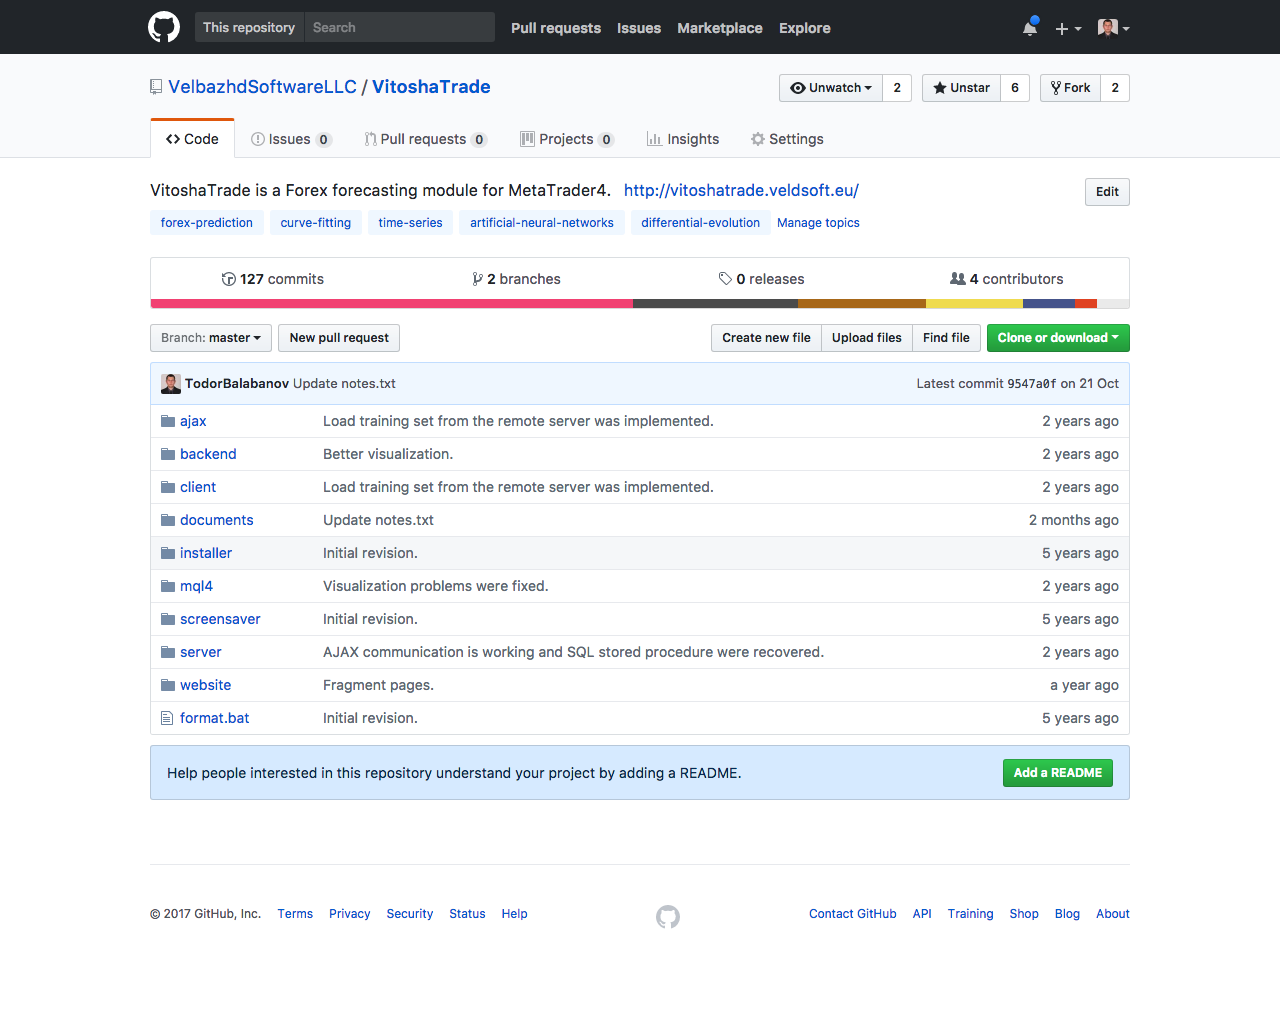
\includegraphics[height=0.45\pdfpageheight]{pic0095}
\caption{Public repository for server application code}
\label{fig:pic0095}
\end{figure}
\FloatBarrier

\section{Relational Database}

For the needs of storing information on the server side, it is sufficient to develop a database in which the tables are normalized to at least third normal form (Fig. \ref{fig:pic0096}).

\begin{figure}[h]
\centering
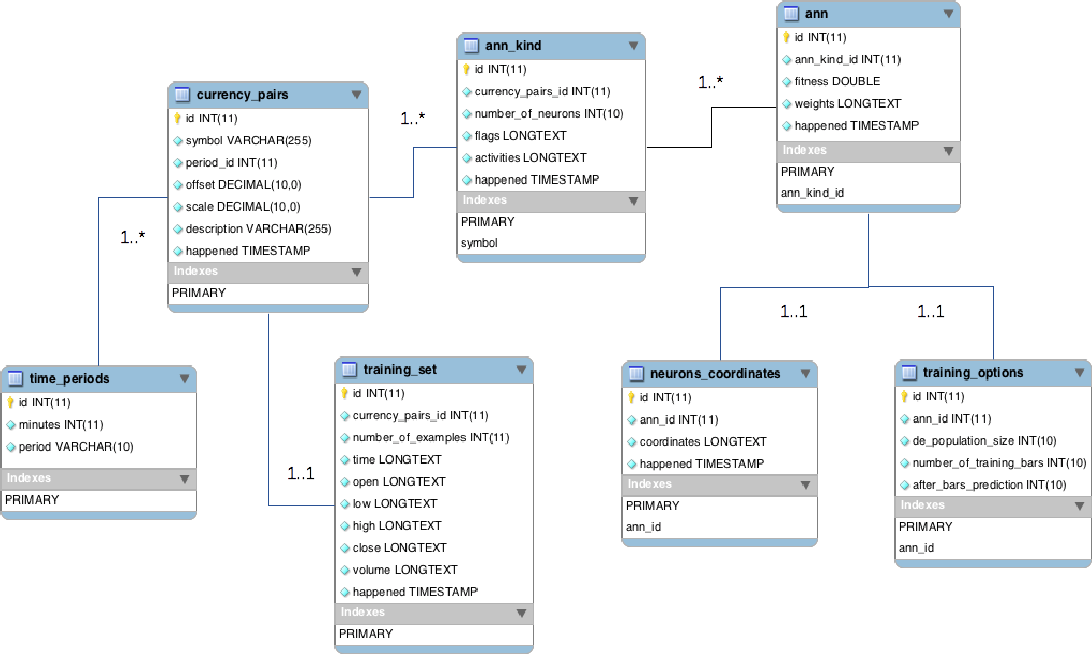
\includegraphics[height=0.35\pdfpageheight]{pic0096}
\caption{Physical structure of the database}
\label{fig:pic0096}
\end{figure}
\FloatBarrier

What each financial time series has is an interval at which level readings are made. This information is recorded in a table with three columns - service identifier, number of minutes for the interval and symbolic name of the interval (Fig. \ref{fig:pic0097}).

\begin{figure}[h]
\centering
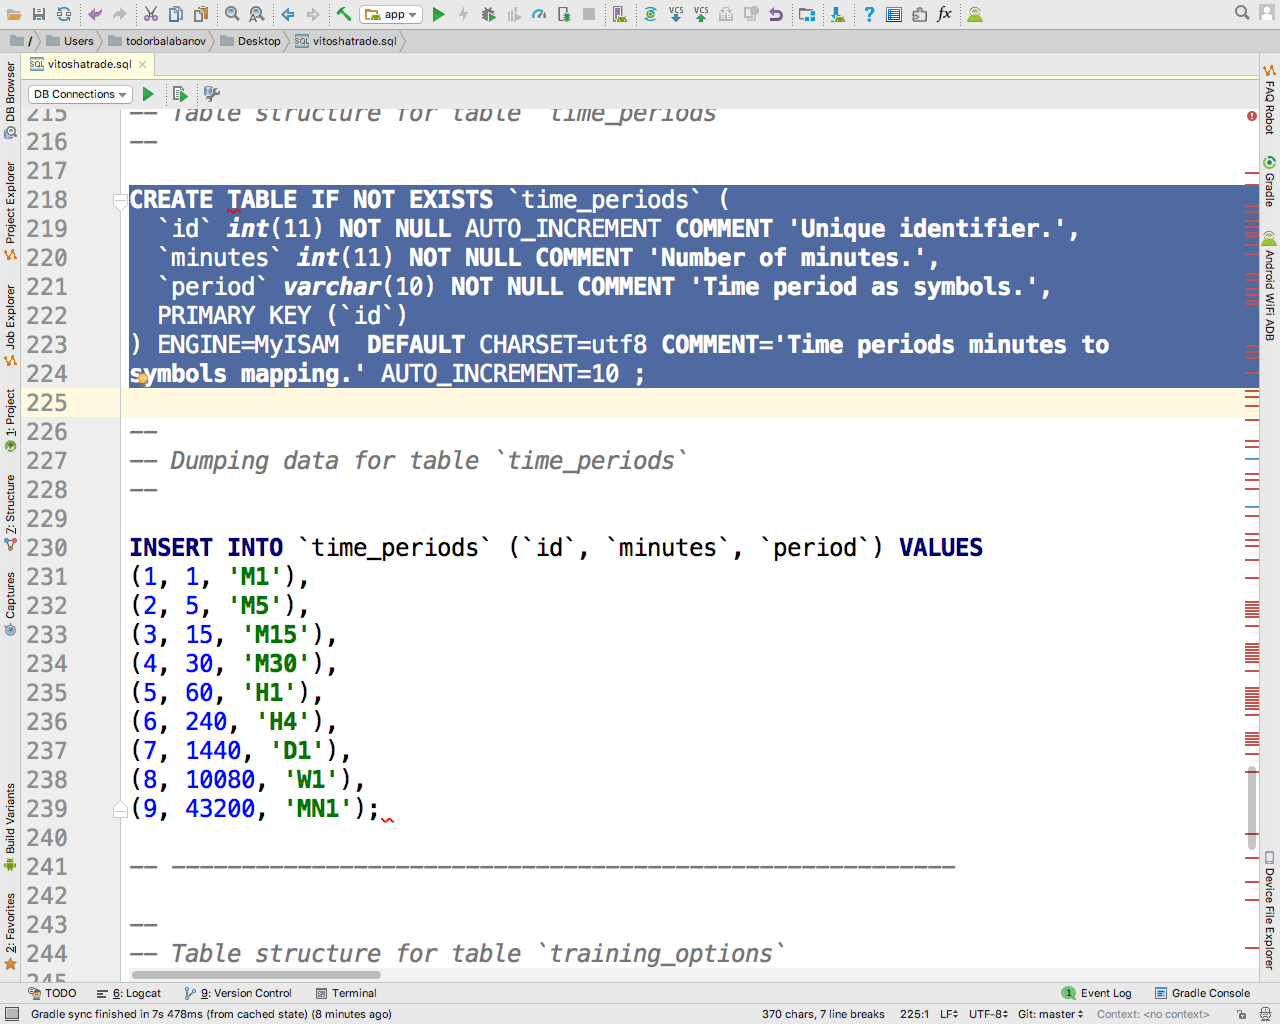
\includegraphics[height=0.45\pdfpageheight]{pic0097}
\caption{Table with the time intervals for the rows}
\label{fig:pic0097}
\end{figure}
\FloatBarrier

The most important table in the database is the table for describing the currency pairs (Fig. \ref{fig:pic0098}). It contains the following fields - service identifier, name of the currency pair, foreign key to the time interval, offset required to normalize the information, scaling factor also required for the normalization of the information, description of the currency pair and time marker in which it is table entry made.

\begin{figure}[h]
\centering
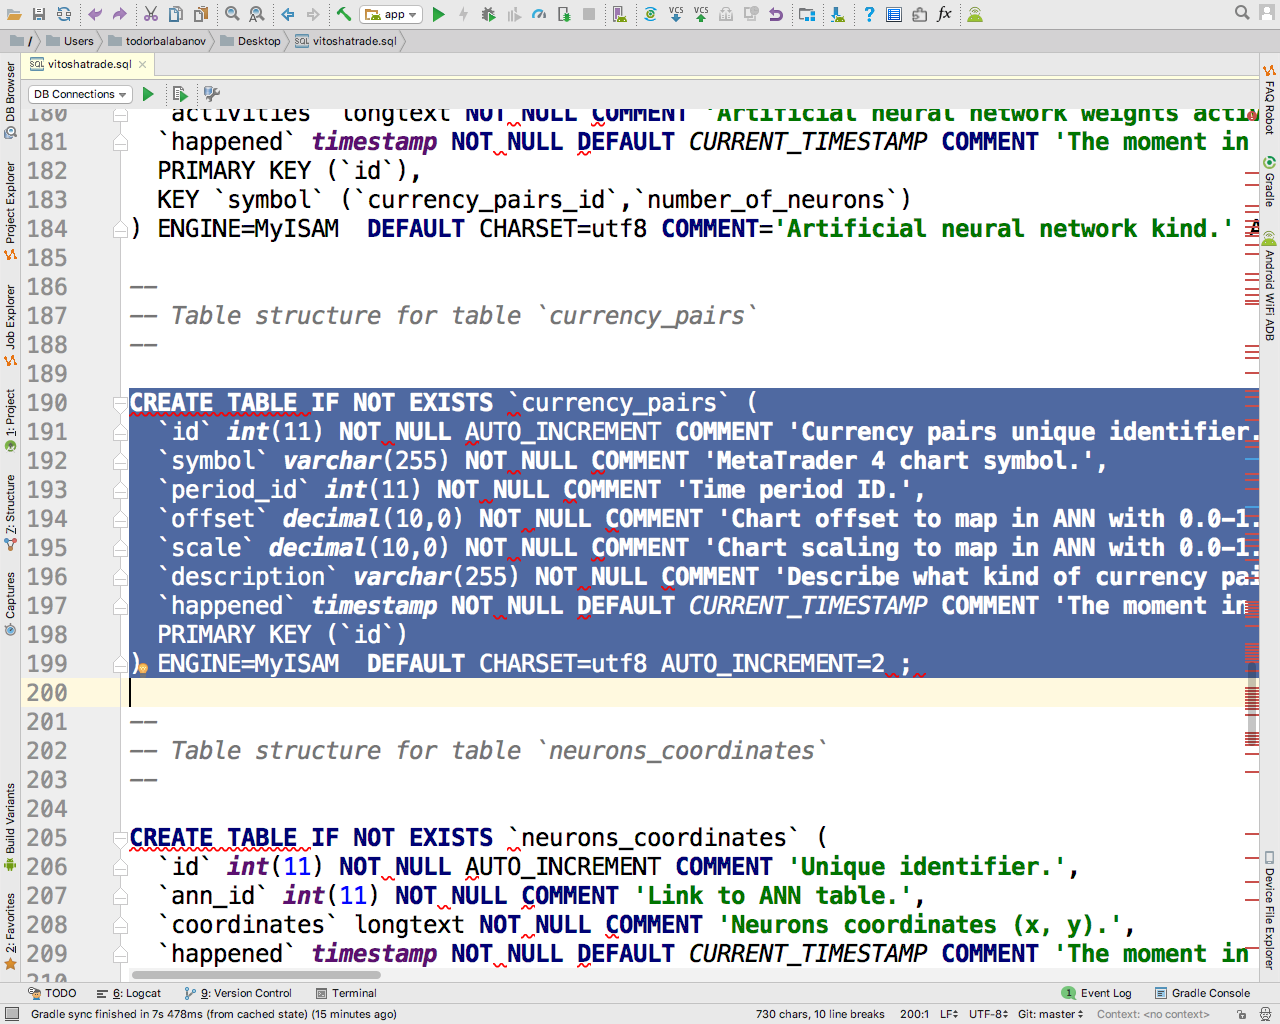
\includegraphics[height=0.45\pdfpageheight]{pic0098}
\caption{Currency pairs presentation table}
\label{fig:pic0098}
\end{figure}
\FloatBarrier

The topology of each neural network is described only once in a table of network types (Fig. \ref{fig:pic0099}). This table contains the following fields - service identifier, foreign key to the currency pair to which the network refers, number of neurons, flags for the type of neurons, values for the connections between neurons (according to the adjacency matrix) and at what point in time the entry was made in the table.

\begin{figure}[h]
\centering
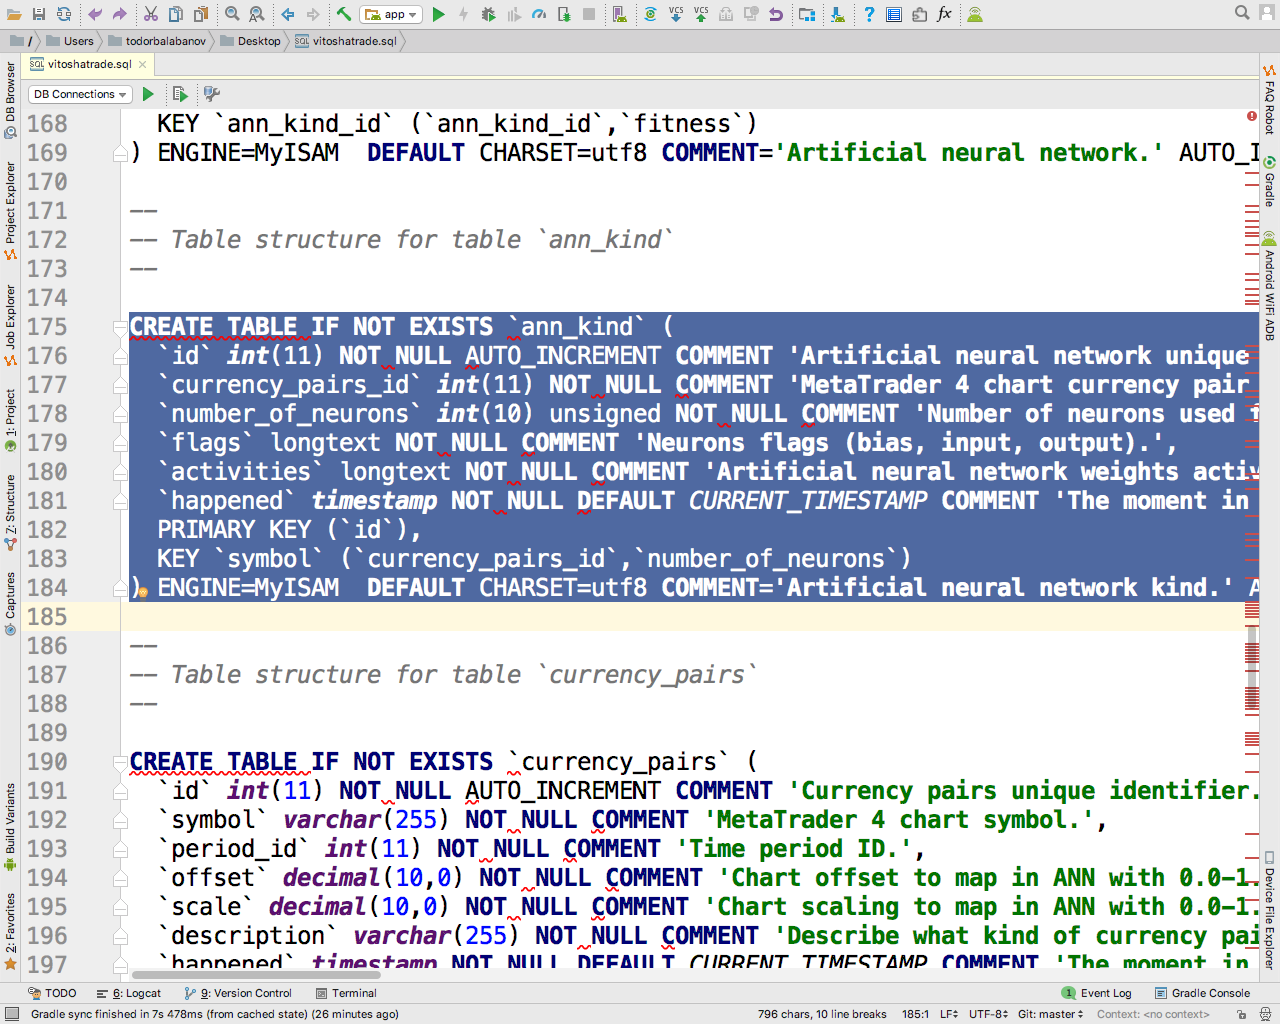
\includegraphics[height=0.45\pdfpageheight]{pic0099}
\caption{Table to represent network types}
\label{fig:pic0099}
\end{figure}
\FloatBarrier

Each network topology may correspond to multiple instances of the artificial neural network type (Fig. \ref{fig:pic0100}). The information in the instance table is organized into the following columns - service identifier, foreign key to the network type to which the instance refers, lifetime value of the instance, weights of connections between neurons (by adjacency graph), and point in time when it was made the entry in the table.

\begin{figure}[h]
\centering
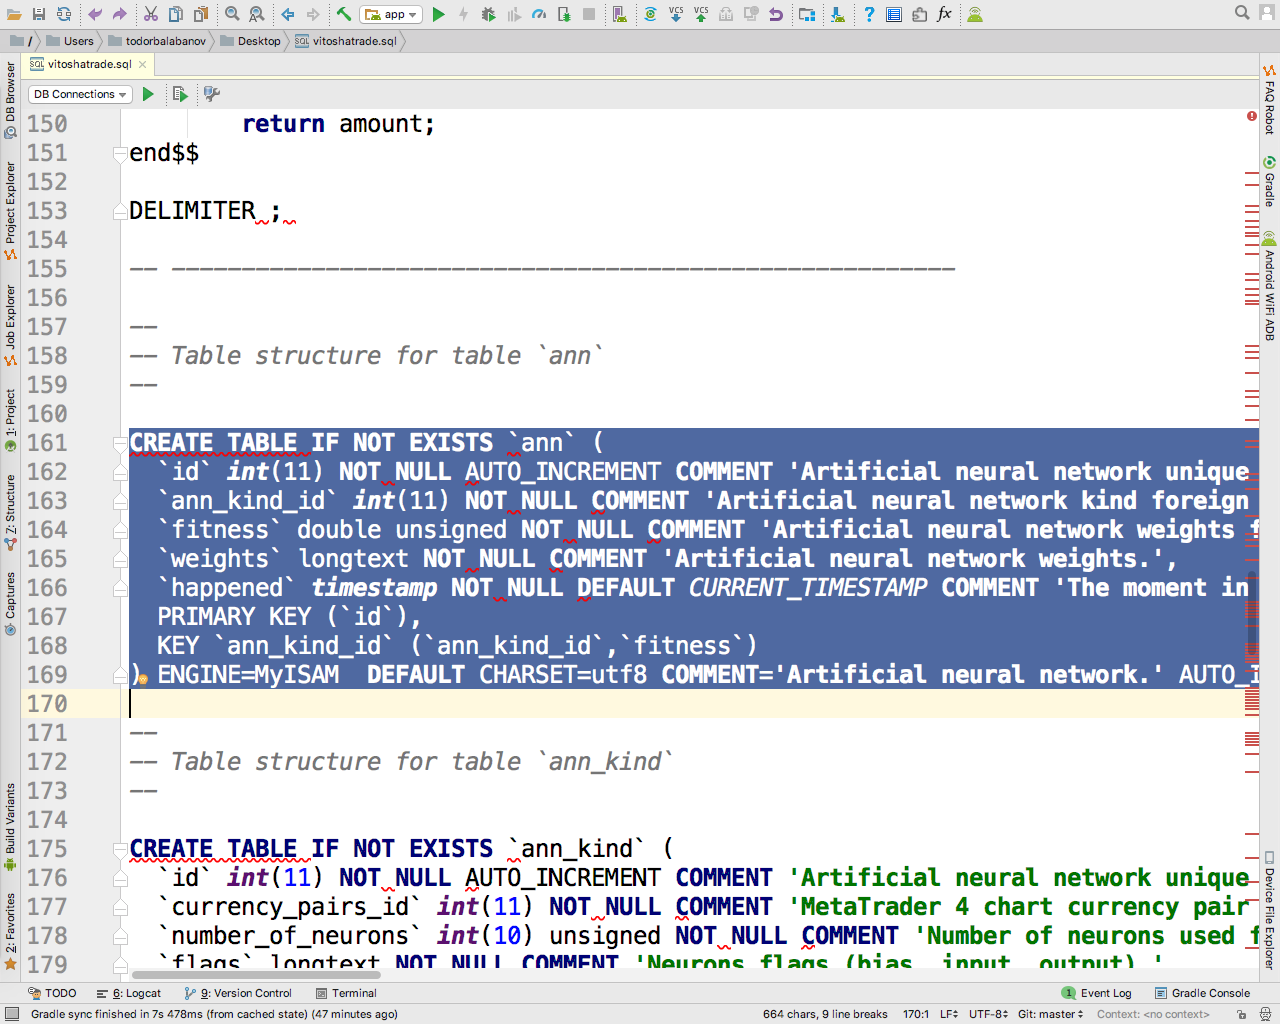
\includegraphics[height=0.45\pdfpageheight]{pic0100}
\caption{Table to represent network types}
\label{fig:pic0100}
\end{figure}
\FloatBarrier

For each instance of a neural network, it is important to know under what parameters its training takes place (Fig. \ref{fig:pic0101}). A separate table with the following columns is intended for this purpose - service identifier, foreign key to the instance, population size (when it comes to a training genetic algorithm), number of bars at the input and number of bars at the output.

\begin{figure}[h]
\centering
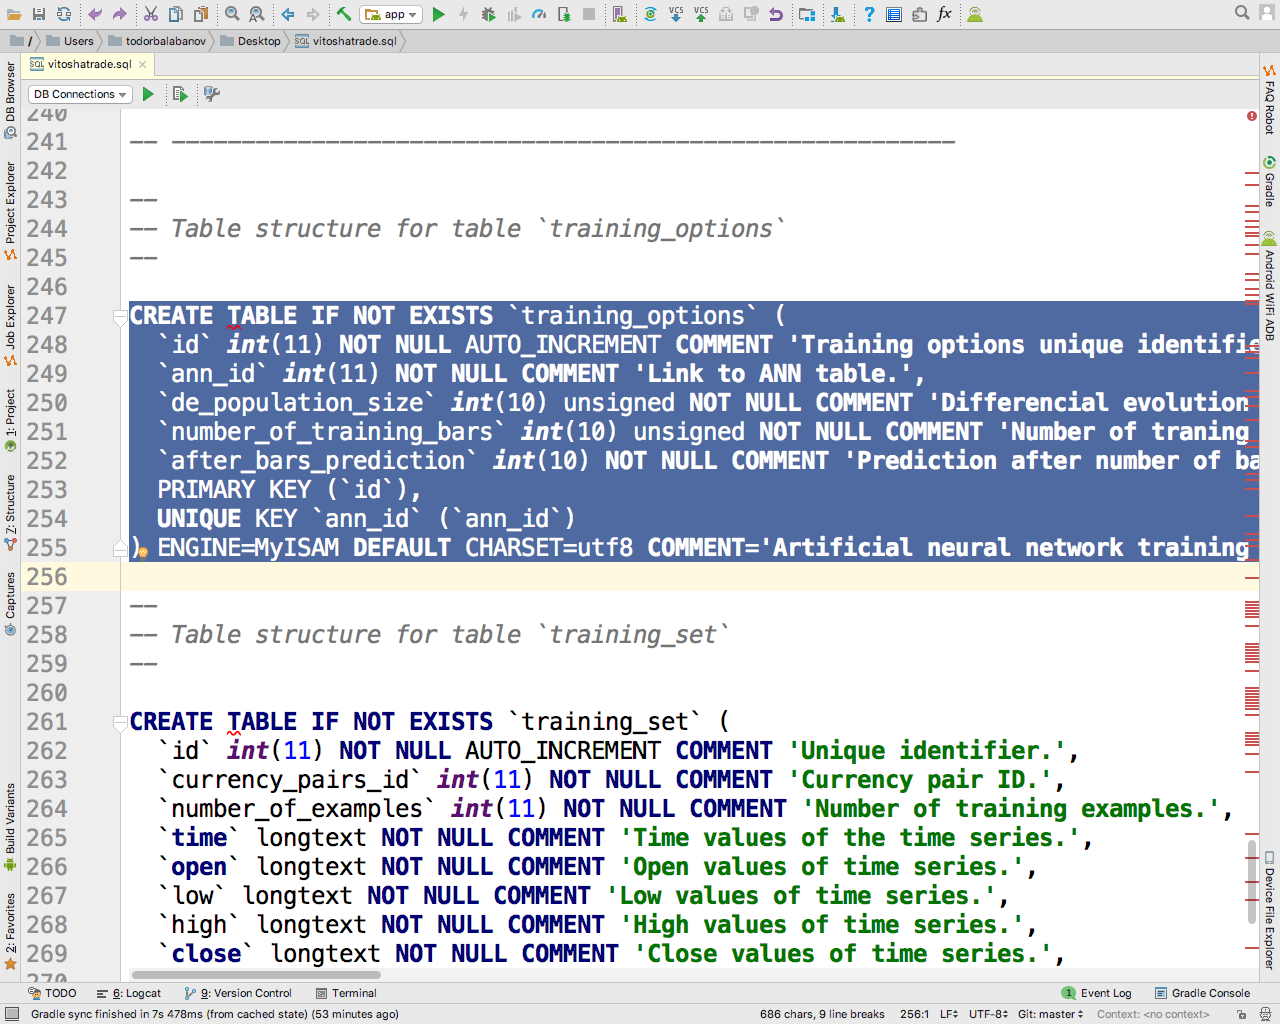
\includegraphics[height=0.45\pdfpageheight]{pic0101}
\caption{Table of learning flow options}
\label{fig:pic0101}
\end{figure}
\FloatBarrier

If you need a visual representation of the instance for an artificial neural network, it is appropriate to store information about the coordinates of each neuron in the xOy plane (Fig. \ref{fig:pic0102}). This table contains the following columns - service identifier, foreign key to the instance, coordinates of the neurons in the order of their occurrence in the instance, and a marker for the time when the entry in the table was made.

\begin{figure}[h]
\centering
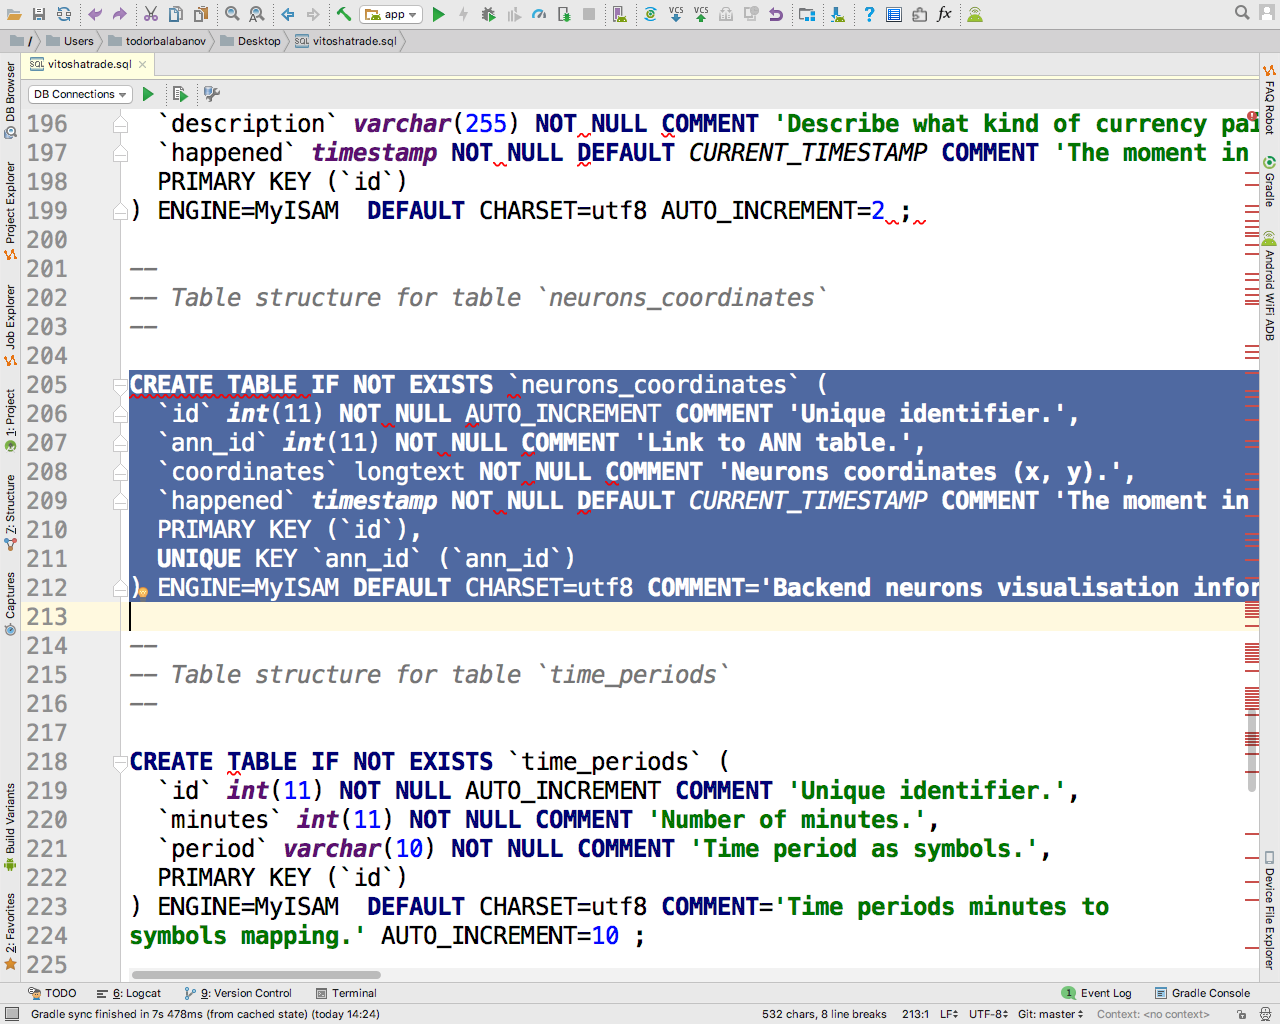
\includegraphics[height=0.45\pdfpageheight]{pic0102}
\caption{Table of learning flow options}
\label{fig:pic0102}
\end{figure}
\FloatBarrier

The last but extremely important table is the table for storing the training examples containing the financial time series information (Fig. \ref{fig:pic0103}). This table contains the following columns - service identifier, foreign key to the currency pair, number of measurements, sequence of timestamps, sequence of levels (open, low, high, close), traded volume and timestamp of the moment when the table entry is made.

\begin{figure}[h]
\centering
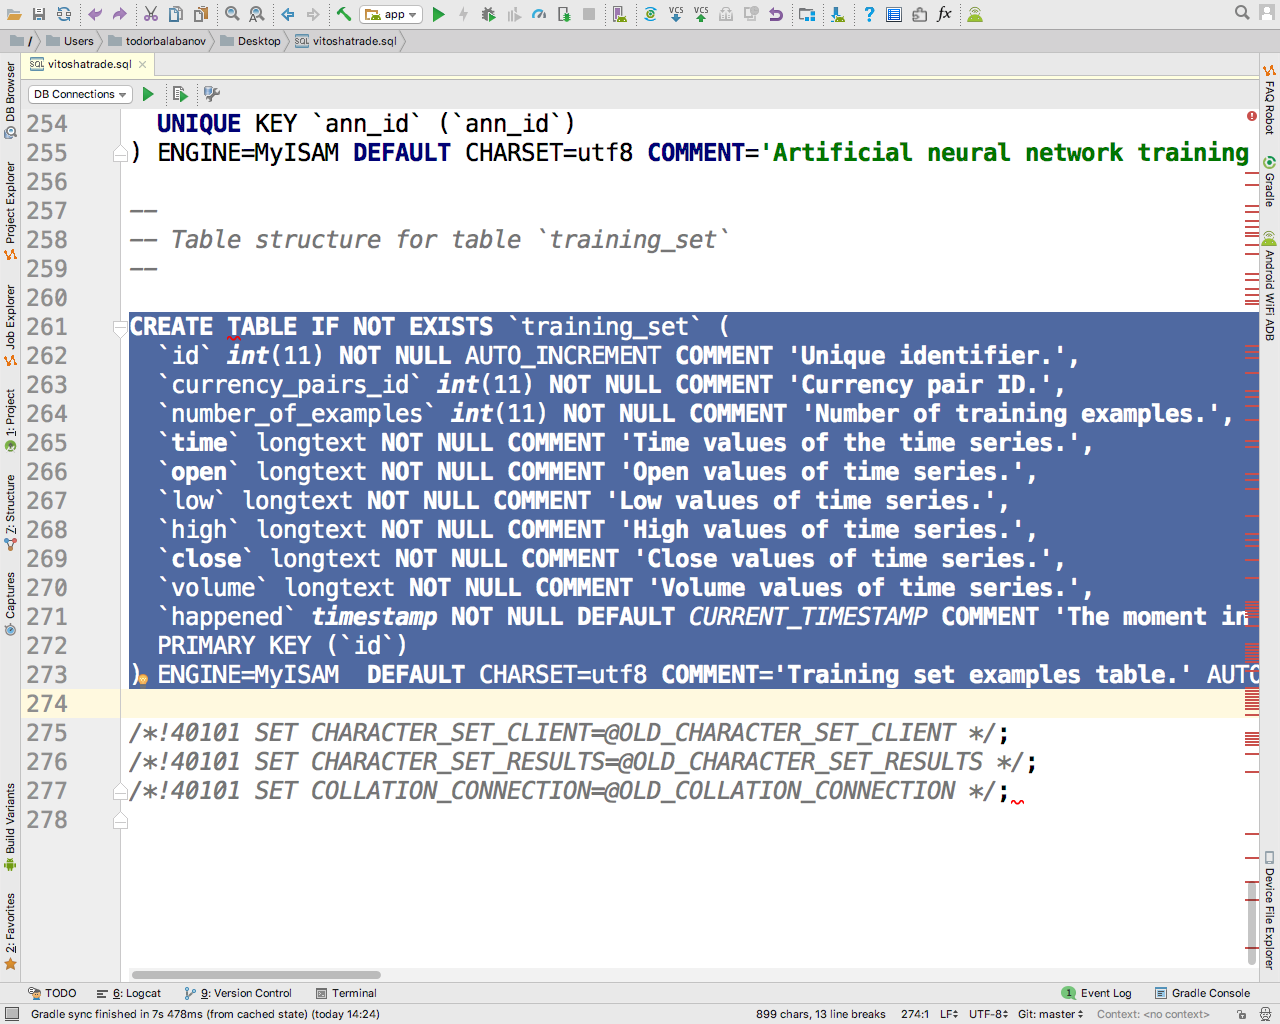
\includegraphics[height=0.45\pdfpageheight]{pic0103}
\caption{Table of learning flow options}
\label{fig:pic0103}
\end{figure}
\FloatBarrier

\section{Algorithmic processing of raw data}

In order to achieve good separation, according to the three-layer architecture of the system, it is essential that the raw data is minimally bound to the working logic. A common practice is to mix the work with the raw data and the program code from the work logic. Such mixing easily occurs if complex SQL queries are executed in work logic scripts. Such a way of constructing the server application makes the system difficult to maintain and even more difficult to reorganize if the database management system or the tools used in the business logic layer need to be changed. A good separation between the two layers occurs when the work logic, in the form of SQL queries, only calls stored functions and procedures (stored procedures) of the database management system. On the one hand, the syntax of requests in the intermediate layer becomes maximally simplified, on the other hand, a possible replacement of the database would lead to a single correction in the way stored functions and procedures are called. To satisfy the drive for maximum separation between layers, a group of stored functions and procedures have been added to the database structure.

\begin{figure}[h]
\centering
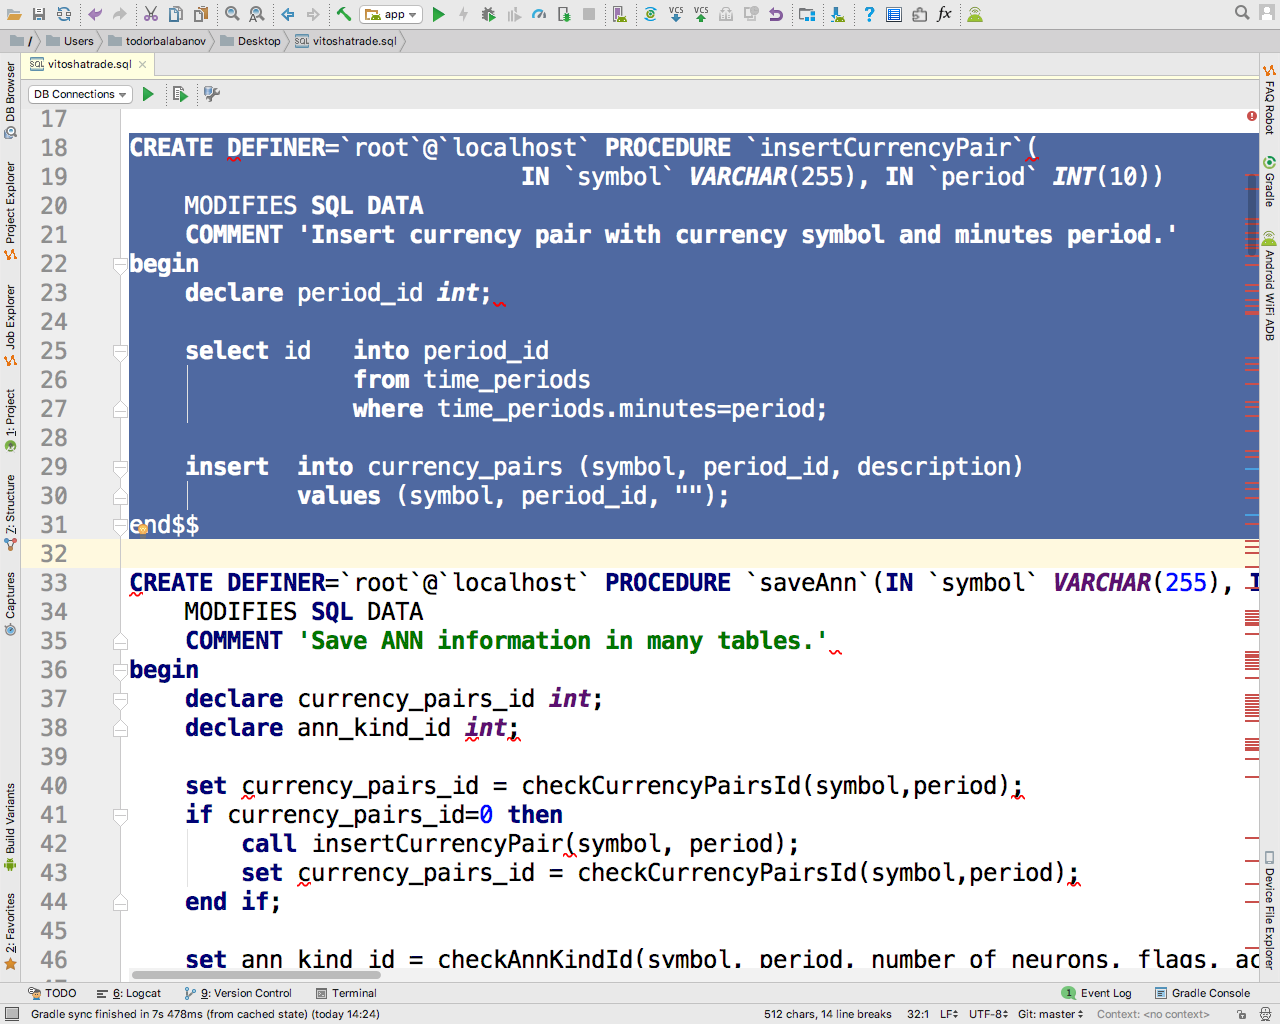
\includegraphics[height=0.45\pdfpageheight]{pic0104}
\caption{Procedure for adding a currency pair}
\label{fig:pic0104}
\end{figure}
\FloatBarrier

When adding a new currency pair, the name of the currency pair and the time interval (in minutes), which interval should be compared to the intervals listed in the table of time intervals, are entered as input data. This necessitates the use of a stored procedure to handle the input information (Fig. \ref{fig:pic0104}).

\begin{figure}[h]
\centering
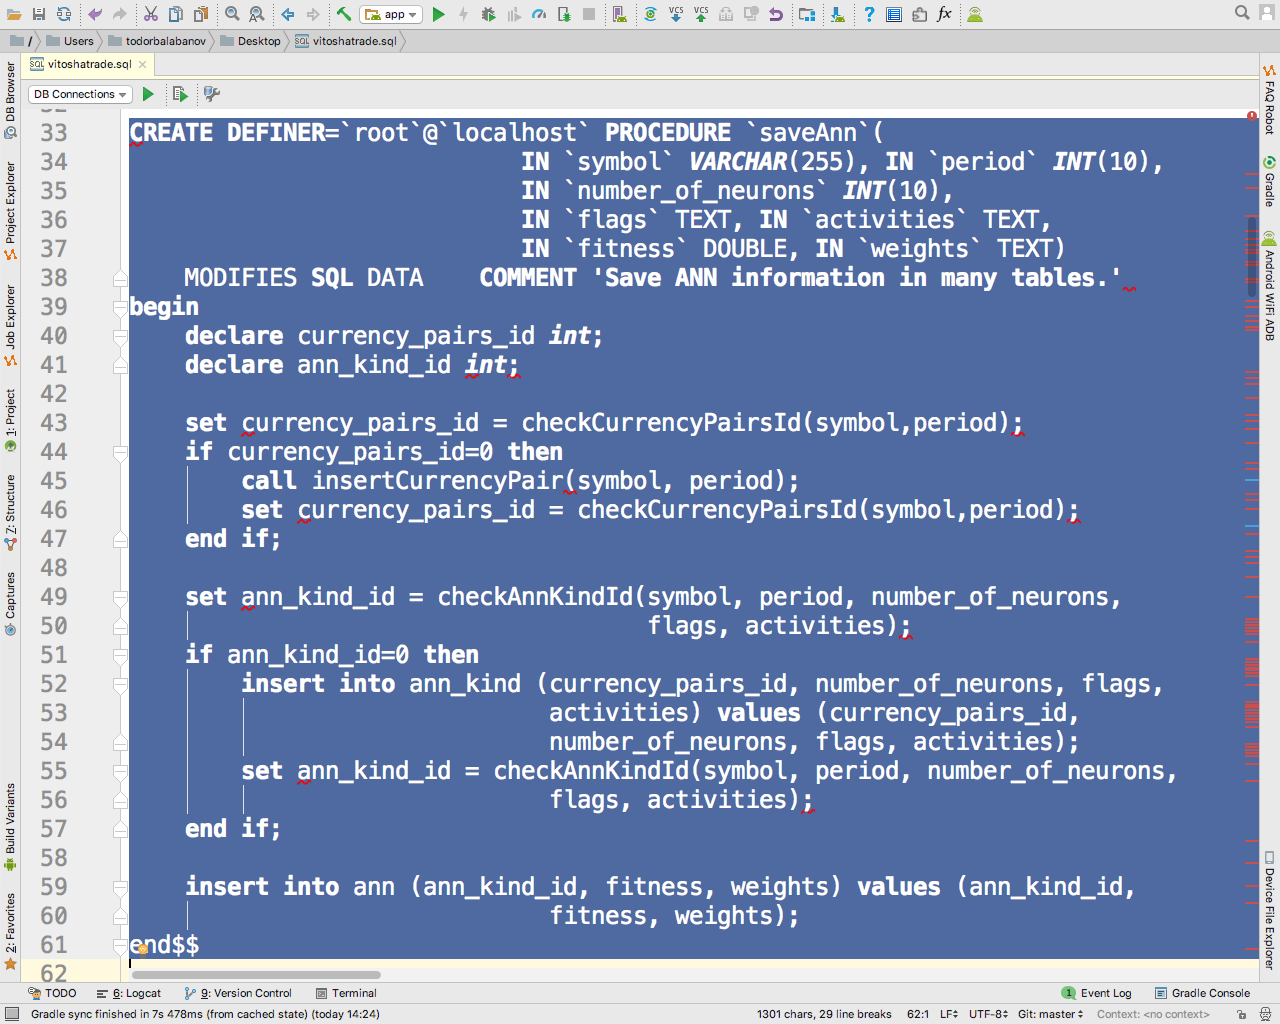
\includegraphics[height=0.45\pdfpageheight]{pic0105}
\caption{Procedure for recording an instance of an artificial neural network}
\label{fig:pic0105}
\end{figure}
\FloatBarrier

When saving an instance of an artificial neural network, the database receives information about the currency pair, the period of the time series, the number and types of neurons, adjacency matrices for the connections, and a live score of the instance (Fig. \ref{fig:pic0105}) . Before the instance is added to the instance table, it is checked whether the currency sucker is available and its identifier is determined. If the currency pair is not available, it is created. Next is a check for the existence of the network type. If it does not exist, it is created. The last instruction is to add the instance itself to the instance table. With the work strategy chosen in this way, the rules for observing referential integrity are observed as much as possible.

\begin{figure}[h]
\centering
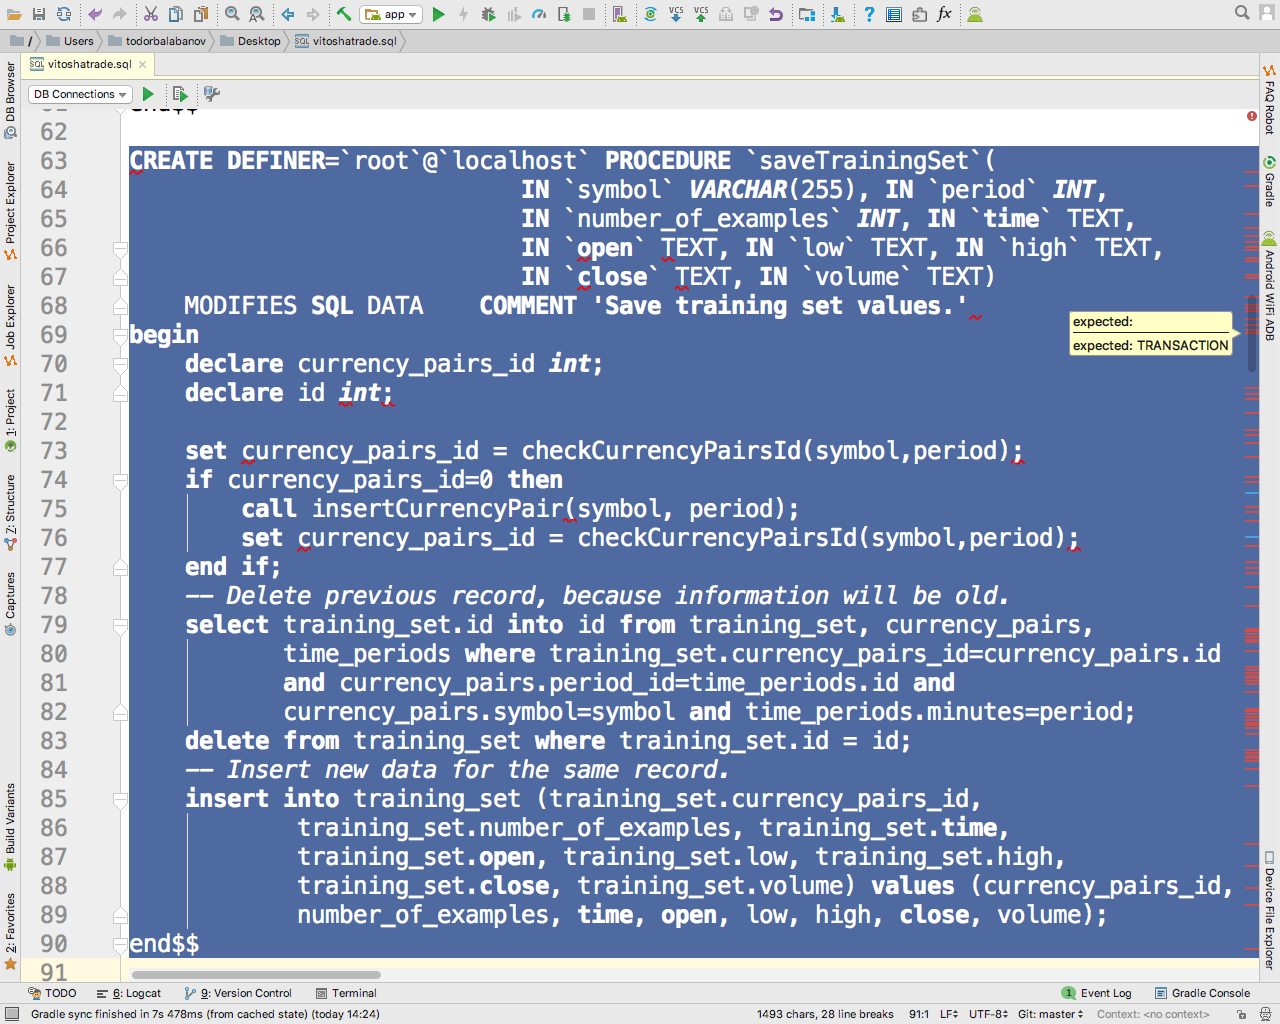
\includegraphics[height=0.45\pdfpageheight]{pic0106}
\caption{Procedure for recording training examples}
\label{fig:pic0106}
\end{figure}
\FloatBarrier

When recording training examples, a series of time series value parameters are fed to the database input (Fig. \ref{fig:pic0106}). In an analogous way, a check for the existence of the currency pair is carried out. This is followed by deletion of previous training examples if any are found. The final step is adding the received information.

\begin{figure}[h]
\centering
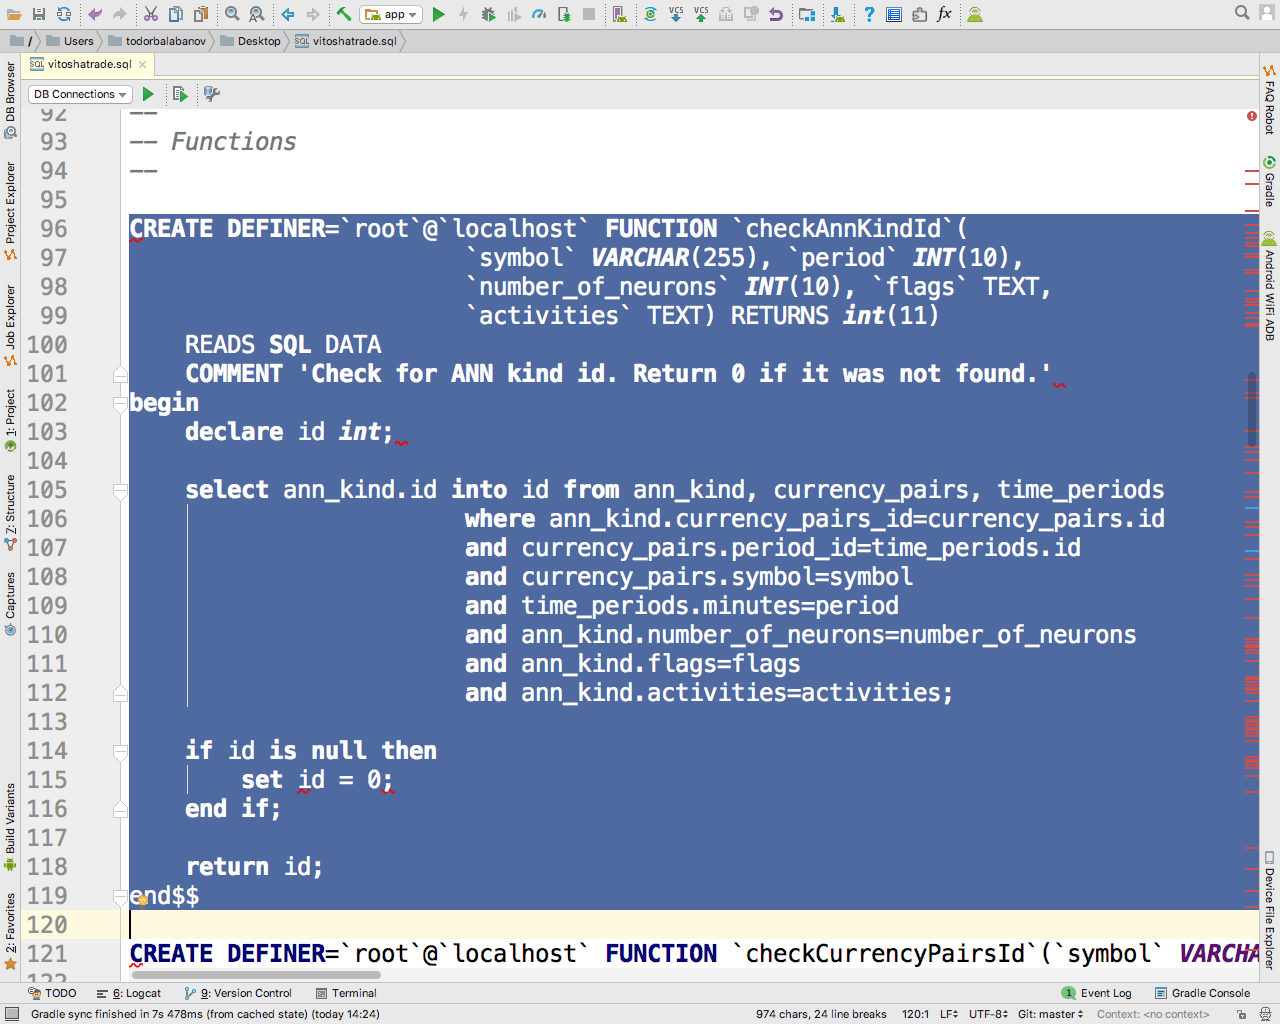
\includegraphics[height=0.45\pdfpageheight]{pic0107}
\caption{Function to determine network type}
\label{fig:pic0107}
\end{figure}
\FloatBarrier

A helper function determines the service identifier of the network type from the instance description (Fig. \ref{fig:pic0107}). If no such type is found, a null value is automatically returned.

\begin{figure}[h]
\centering
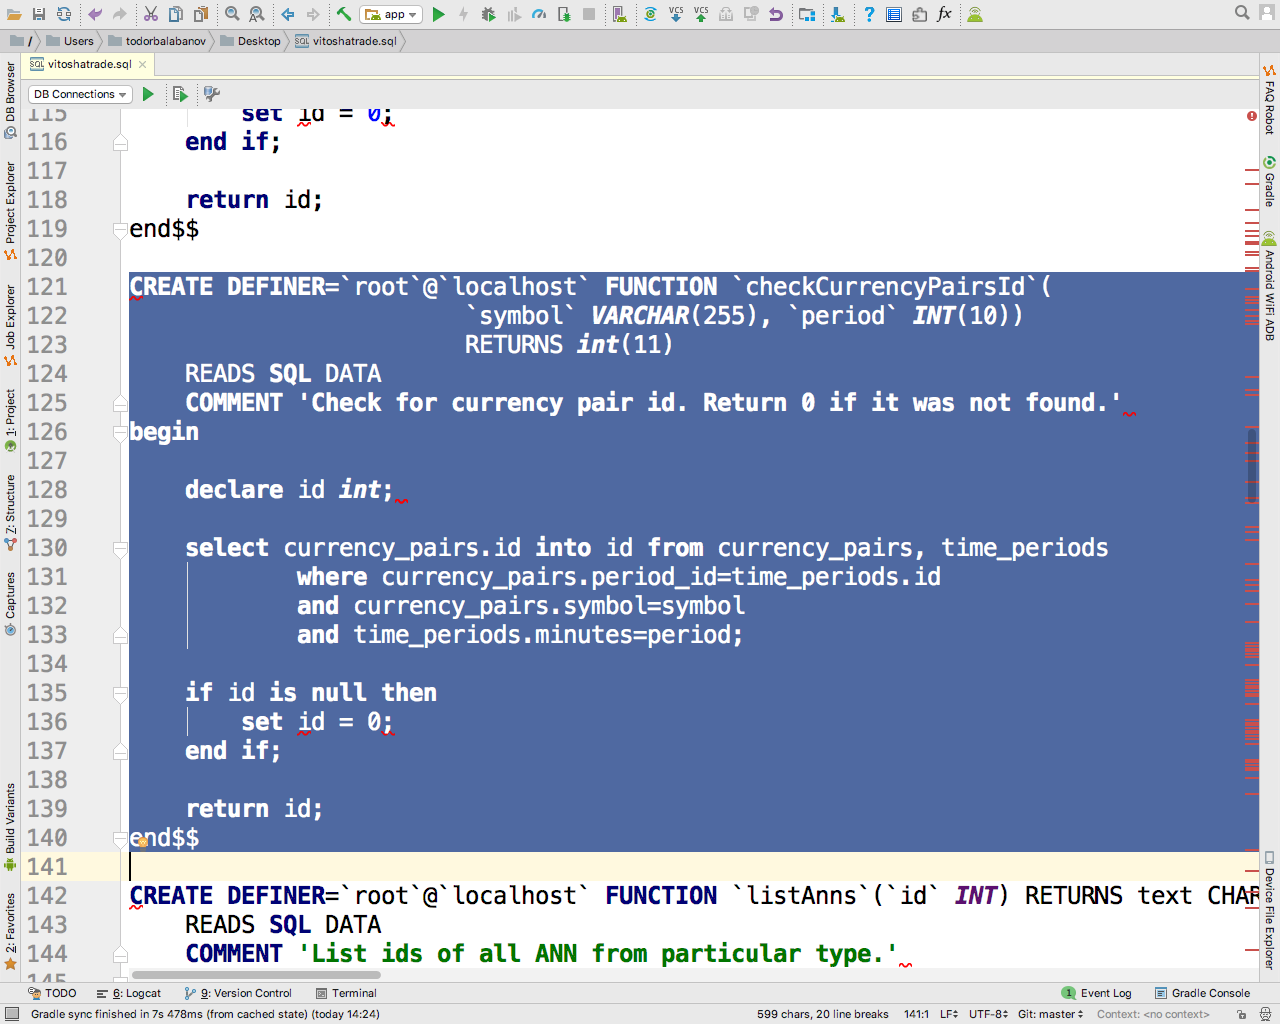
\includegraphics[height=0.45\pdfpageheight]{pic0108}
\caption{Function to determine currency pair type}
\label{fig:pic0108}
\end{figure}
\FloatBarrier

Similarly, a helper function serves to determine the service identifier for a currency pair, by means of a given symbol name and period (Fig. \ref{fig:pic0108}). If the currency pair is not found, a service zero is returned.

\begin{figure}[h]
\centering
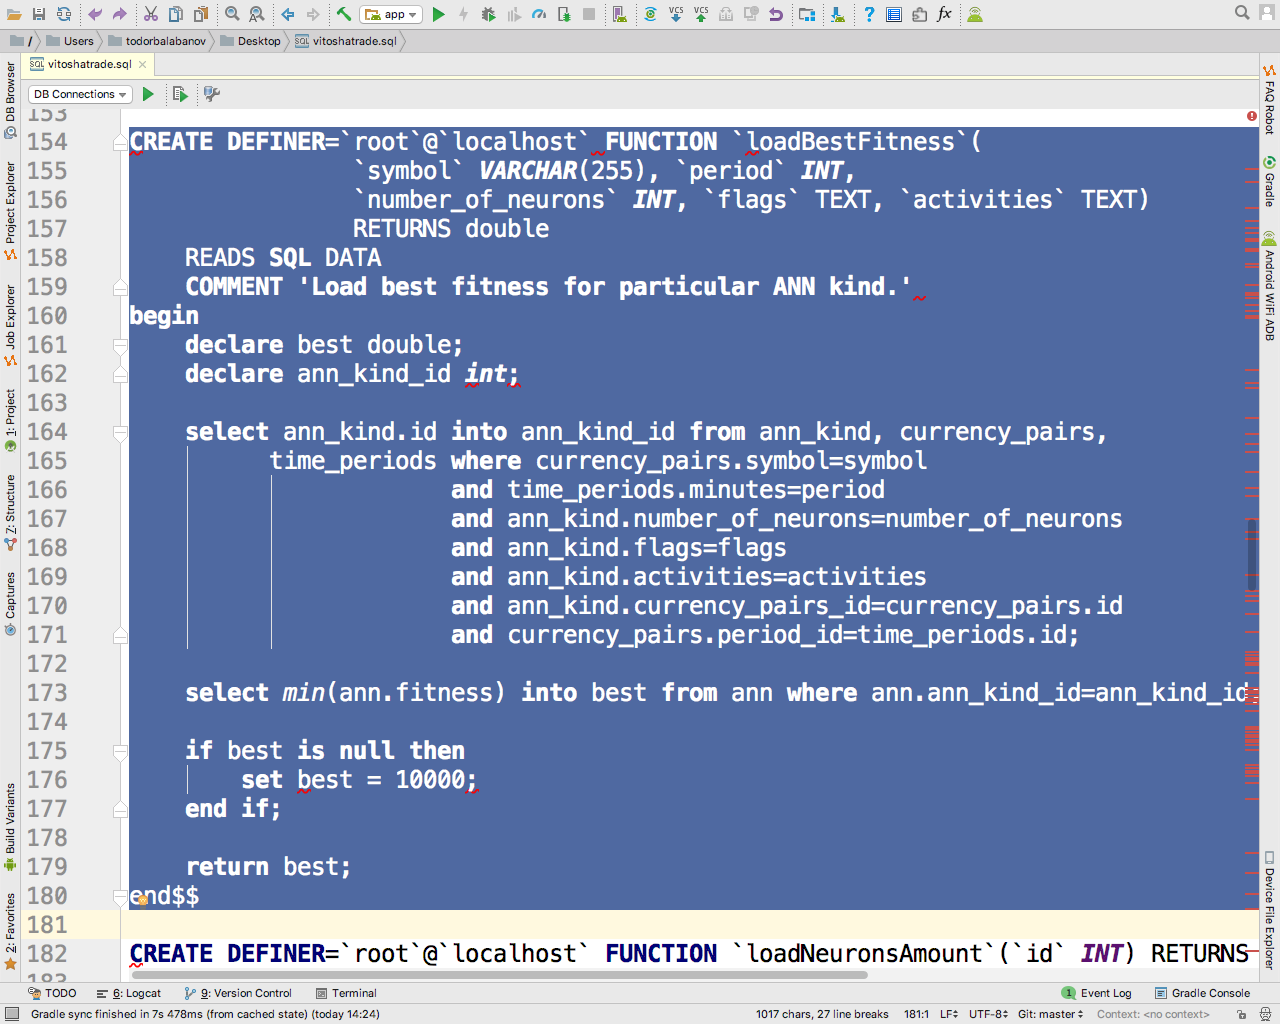
\includegraphics[height=0.45\pdfpageheight]{pic0109}
\caption{Function to determine the best vitality}
\label{fig:pic0109}
\end{figure}
\FloatBarrier

According to a set description of the artificial neural network, the client mobile devices ask the server, at certain time intervals, what is the value of the most vital network. This query is essential because it decides whether the mobile device should report its results to the server. The processing is done in two steps - first all networks with identical topology are found and then the best liveness is determined (Fig. \ref{fig:pic0109}).

\begin{figure}[h]
\centering
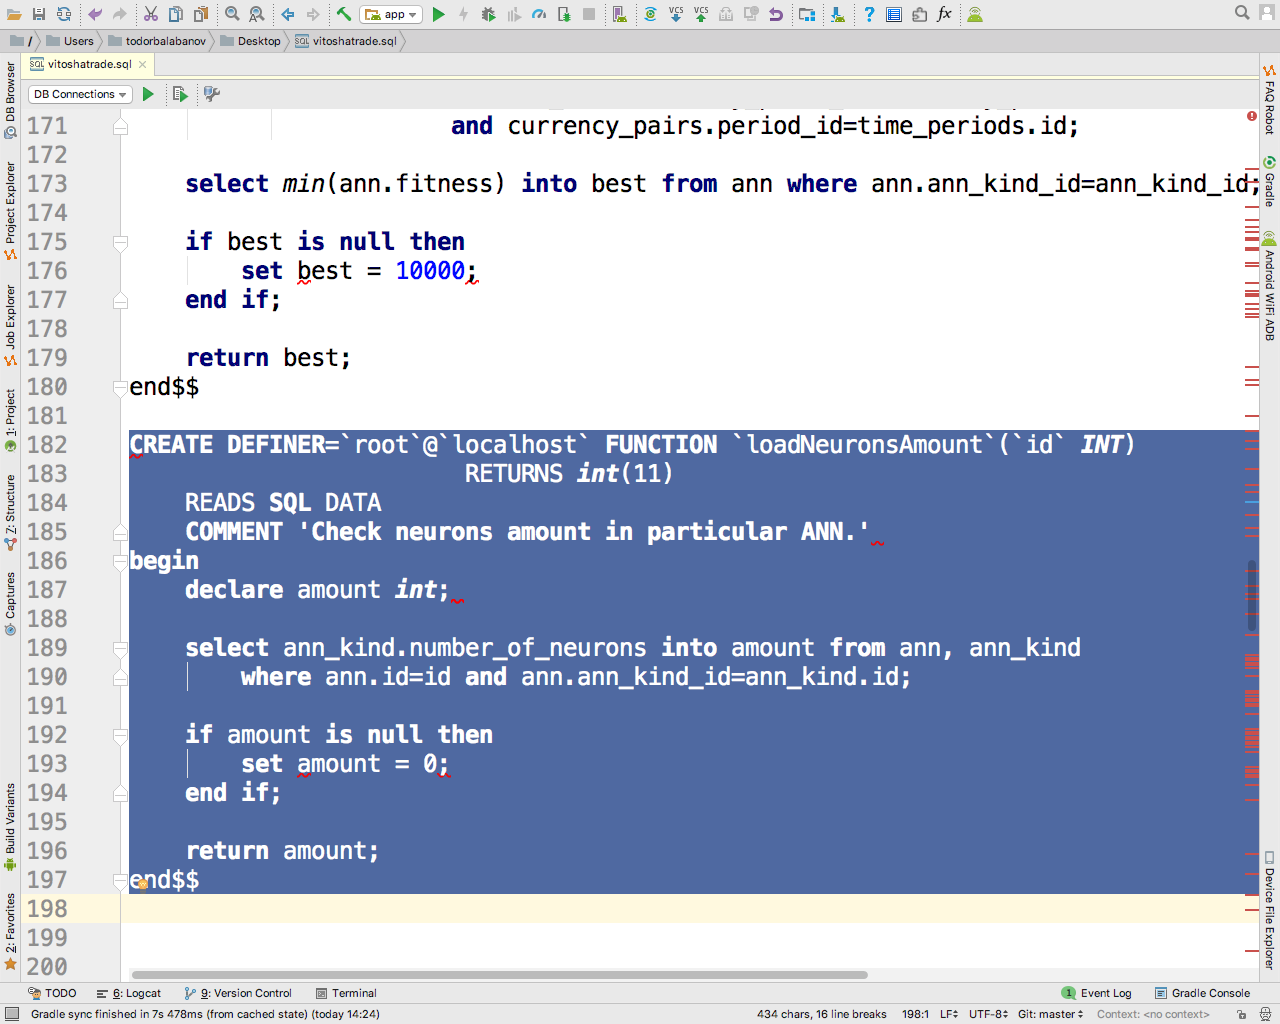
\includegraphics[height=0.45\pdfpageheight]{pic0110}
\caption{Function to determine the number of neurons for a particular network instance}
\label{fig:pic0110}
\end{figure}
\FloatBarrier

A helper function also determines the number of neurons by a given ID of a network instance (Fig. \ref{fig:pic0110}).

\section{Server Scripts}

Direct access to the database (TCP connection) is often undesirable because it creates certain data security hazards. For this reason, it is accepted to use an intermediate layer to communicate with the database. For the purposes of this tutorial, these are a group of PHP scripts.

\begin{figure}[h]
\centering
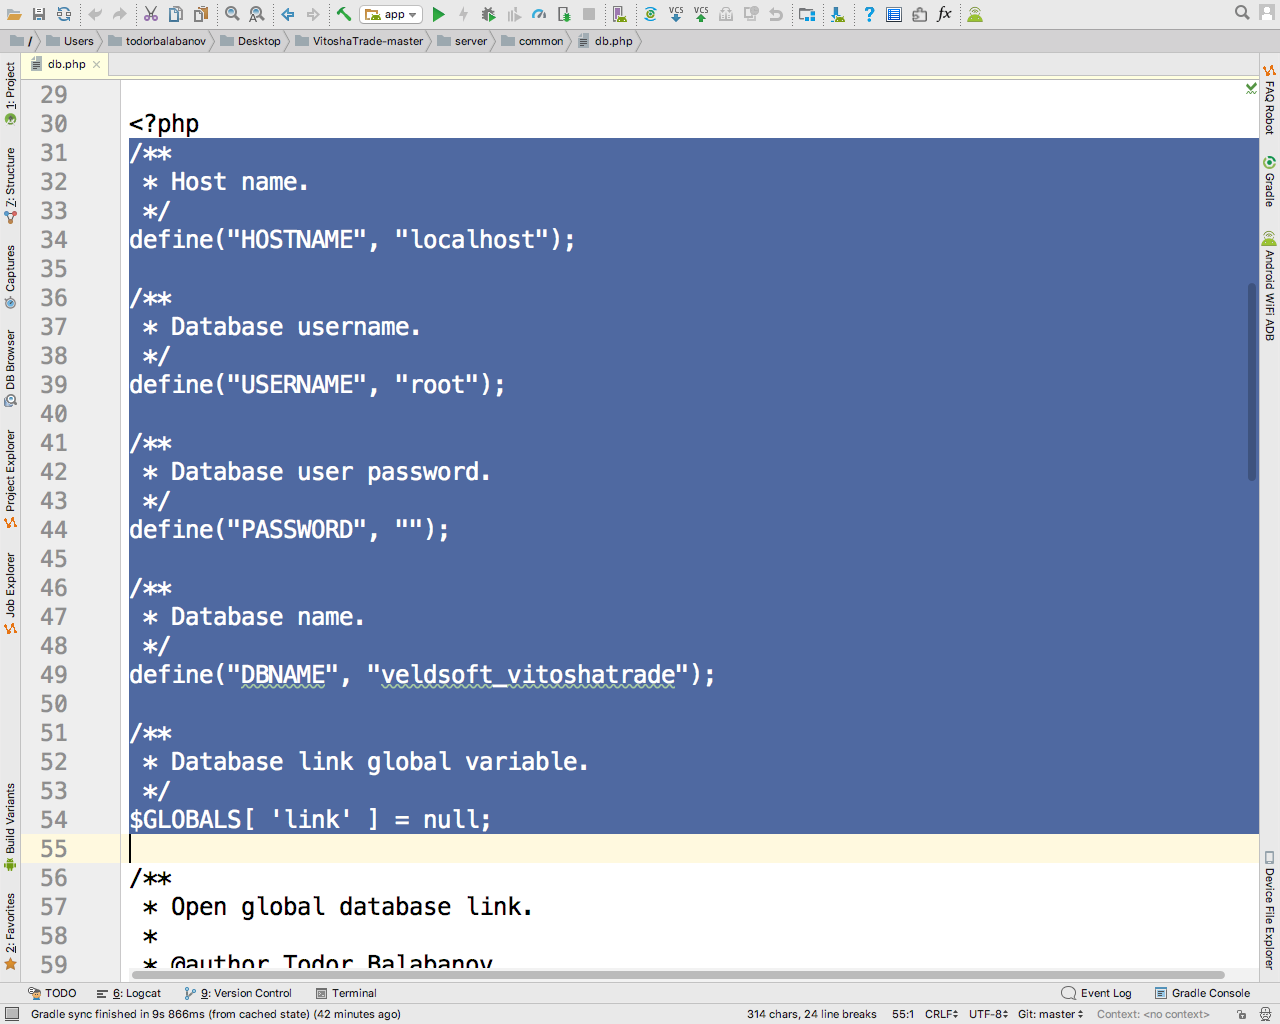
\includegraphics[height=0.45\pdfpageheight]{pic0111}
\caption{Global Database Access Variables}
\label{fig:pic0111}
\end{figure}
\FloatBarrier

In a special file (db.php) set the following global variables for accessing the database - host on which the MySQL server is located, user in MySQL, password of the user, name of the database and connection (Fig. \ref{ fig:pic0111}).

\begin{figure}[h]
\centering
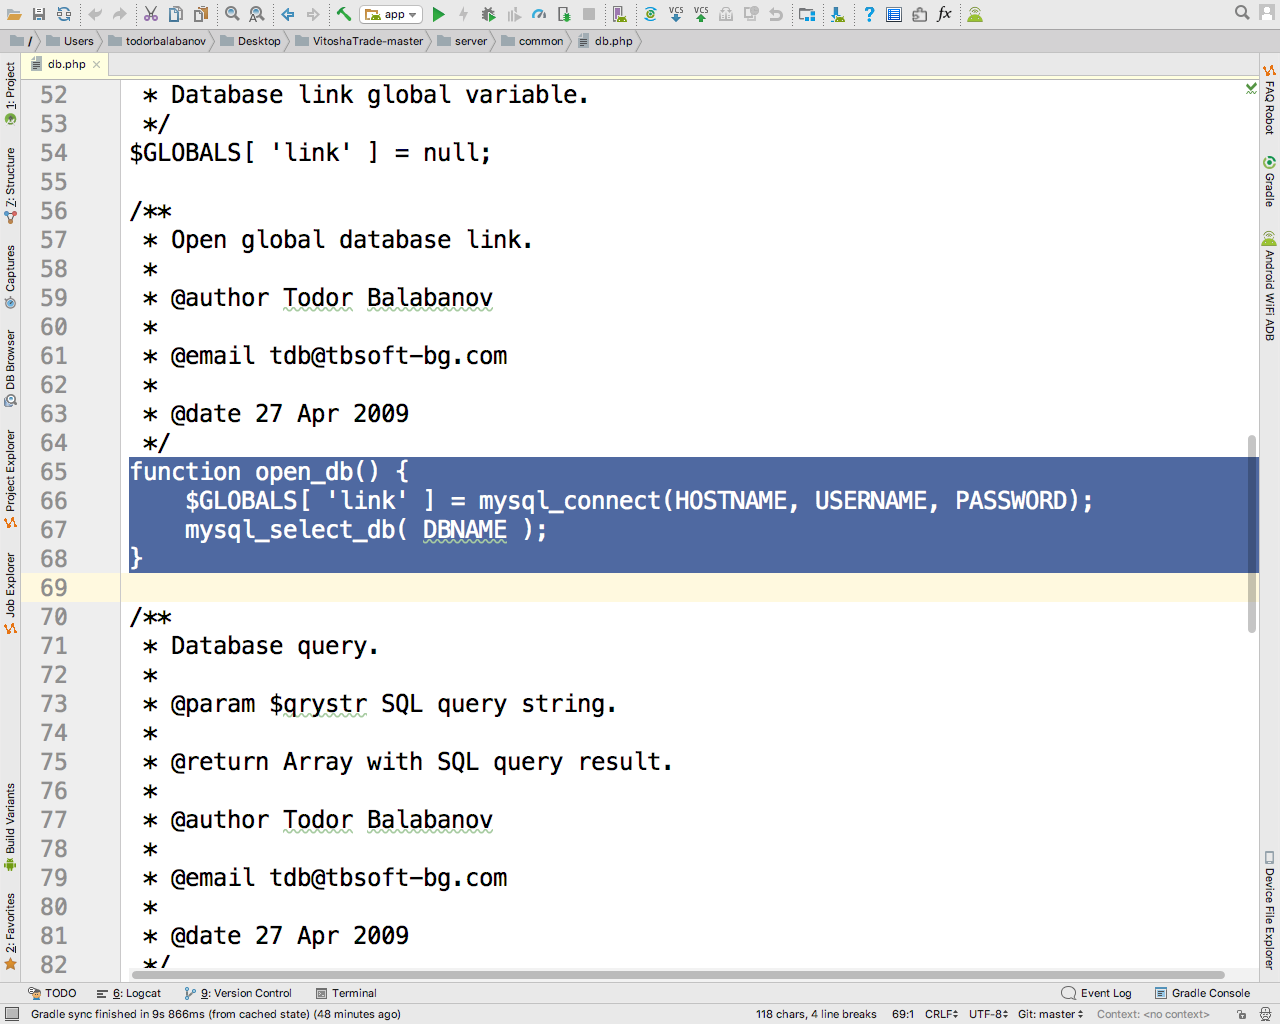
\includegraphics[height=0.45\pdfpageheight]{pic0112}
\caption{Opening database connection}
\label{fig:pic0112}
\end{figure}
\FloatBarrier

Two helper functions serve to open and close a connection to the database (Fig. \ref{fig:pic0112}, \ref{fig:pic0113}).

\begin{figure}[h]
\centering
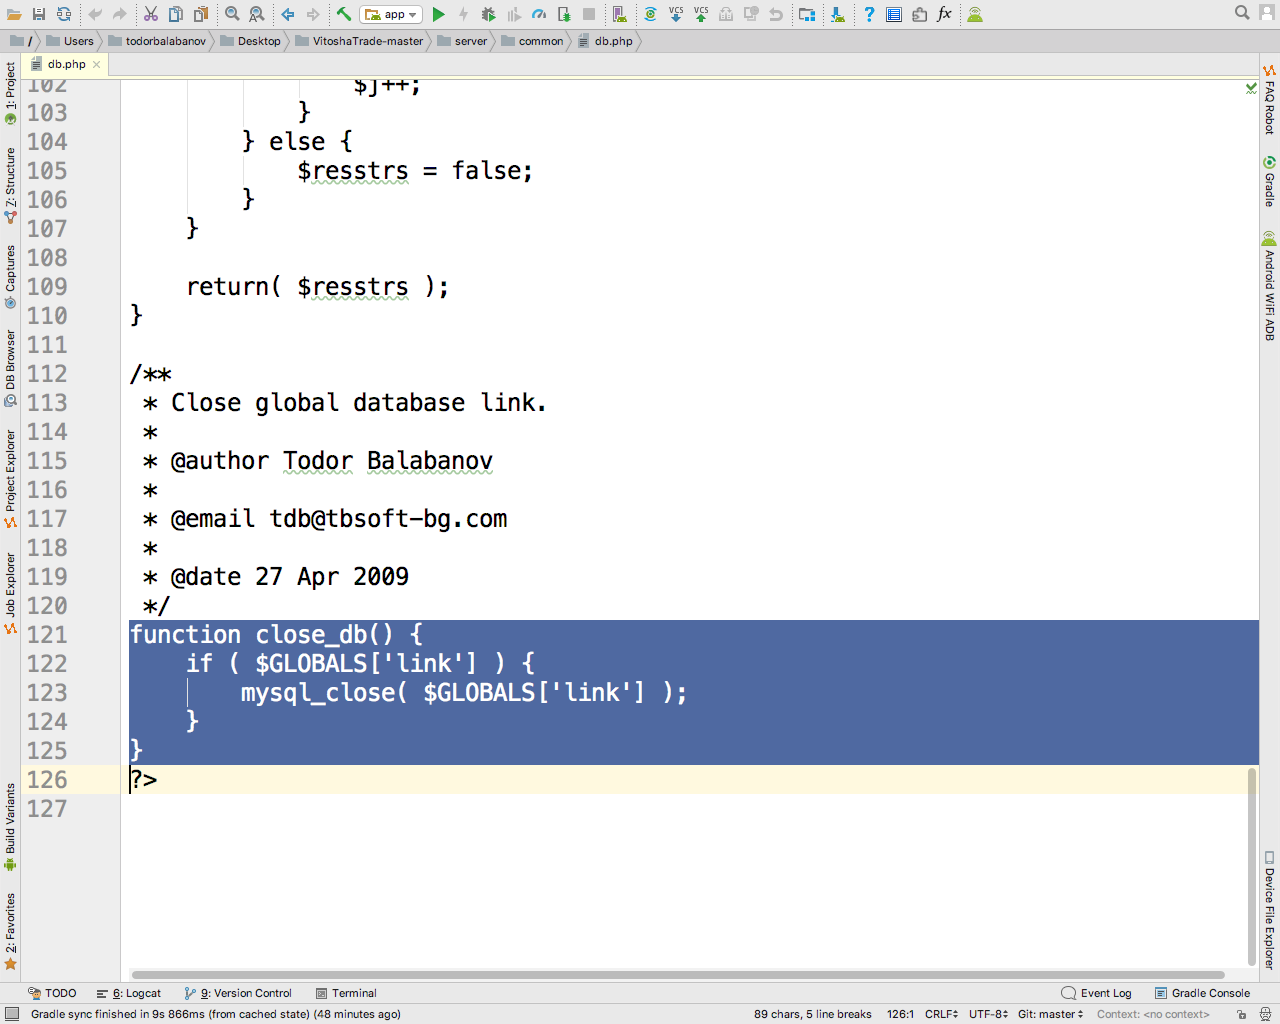
\includegraphics[height=0.45\pdfpageheight]{pic0113}
\caption{Close database connection}
\label{fig:pic0113}
\end{figure}
\FloatBarrier

An additional helper function executes the queries to the database and returns the result of the execution in the form of a two-dimensional array (Fig. \ref{fig:pic0114}).

\begin{figure}[h]
\centering
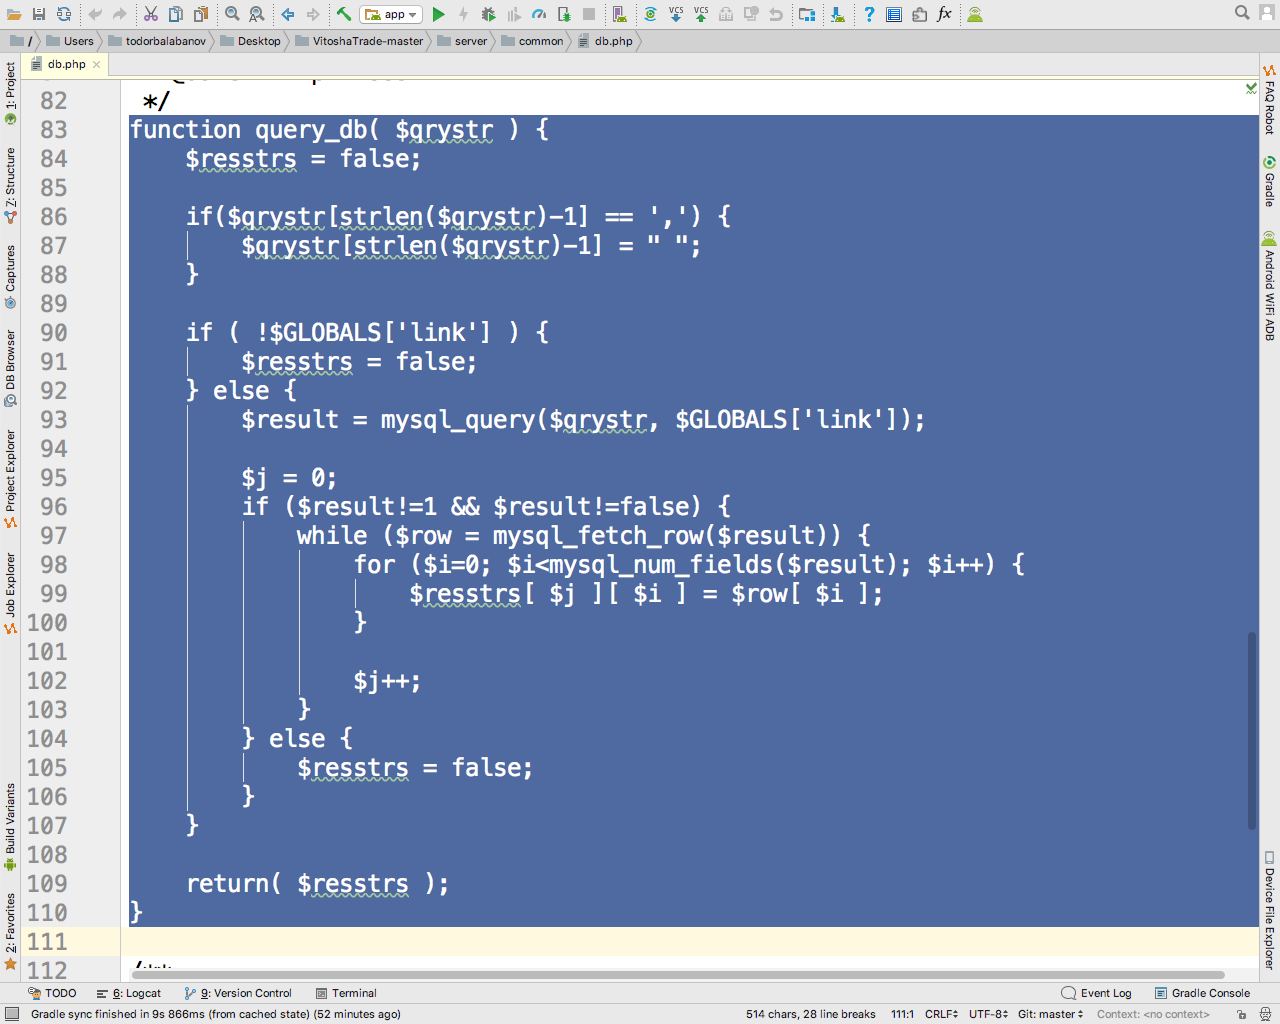
\includegraphics[height=0.45\pdfpageheight]{pic0114}
\caption{Executing Database Queries}
\label{fig:pic0114}
\end{figure}
\FloatBarrier

At this stage in development, the client application sends its data in the form of a POST request, and the server responds with a JSON message. While saving additional work around composing JSON messages on the client side, this approach is not recommended and it is desirable that clients also send the information in JSON format so that the conventions of RESTful applications are respected.

\subsection{Load Grid by ID}

Each instance of an artificial neural network has a service identifier, which is also a primary key in the corresponding table. To load the network, a PHP script is called to perform this task.

\begin{figure}[h]
\centering
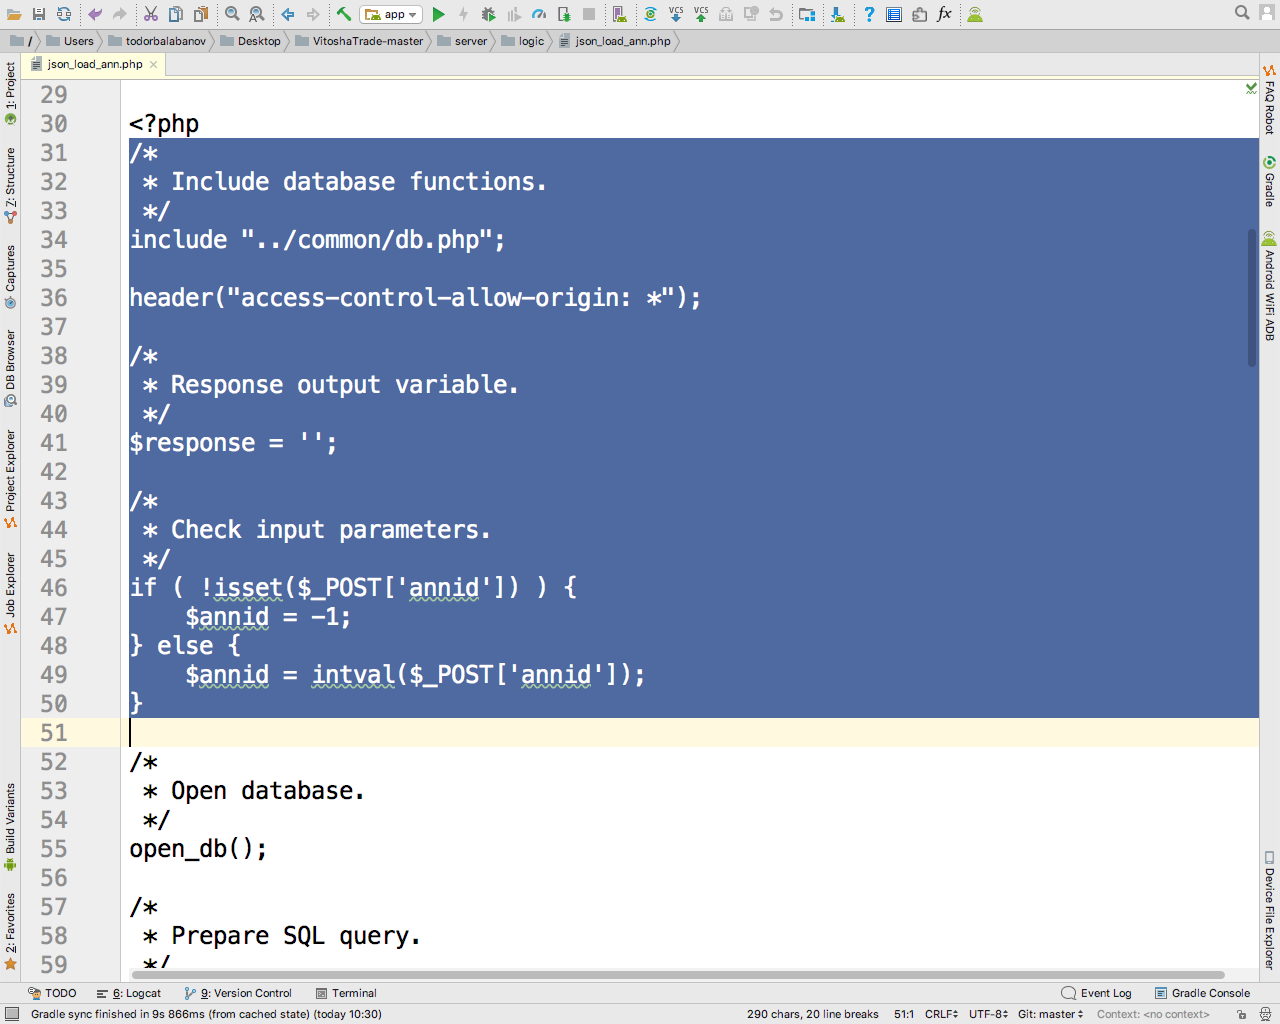
\includegraphics[height=0.45\pdfpageheight]{pic0115}
\caption{Input Verification}
\label{fig:pic0115}
\end{figure}
\FloatBarrier

Before actually loading the network, the database module is turned on and the input parameters are checked. In this case, the only parameter is an integer which is the identifier of the instance (Fig. \ref{fig:pic0115}).

\begin{figure}[h]
\centering
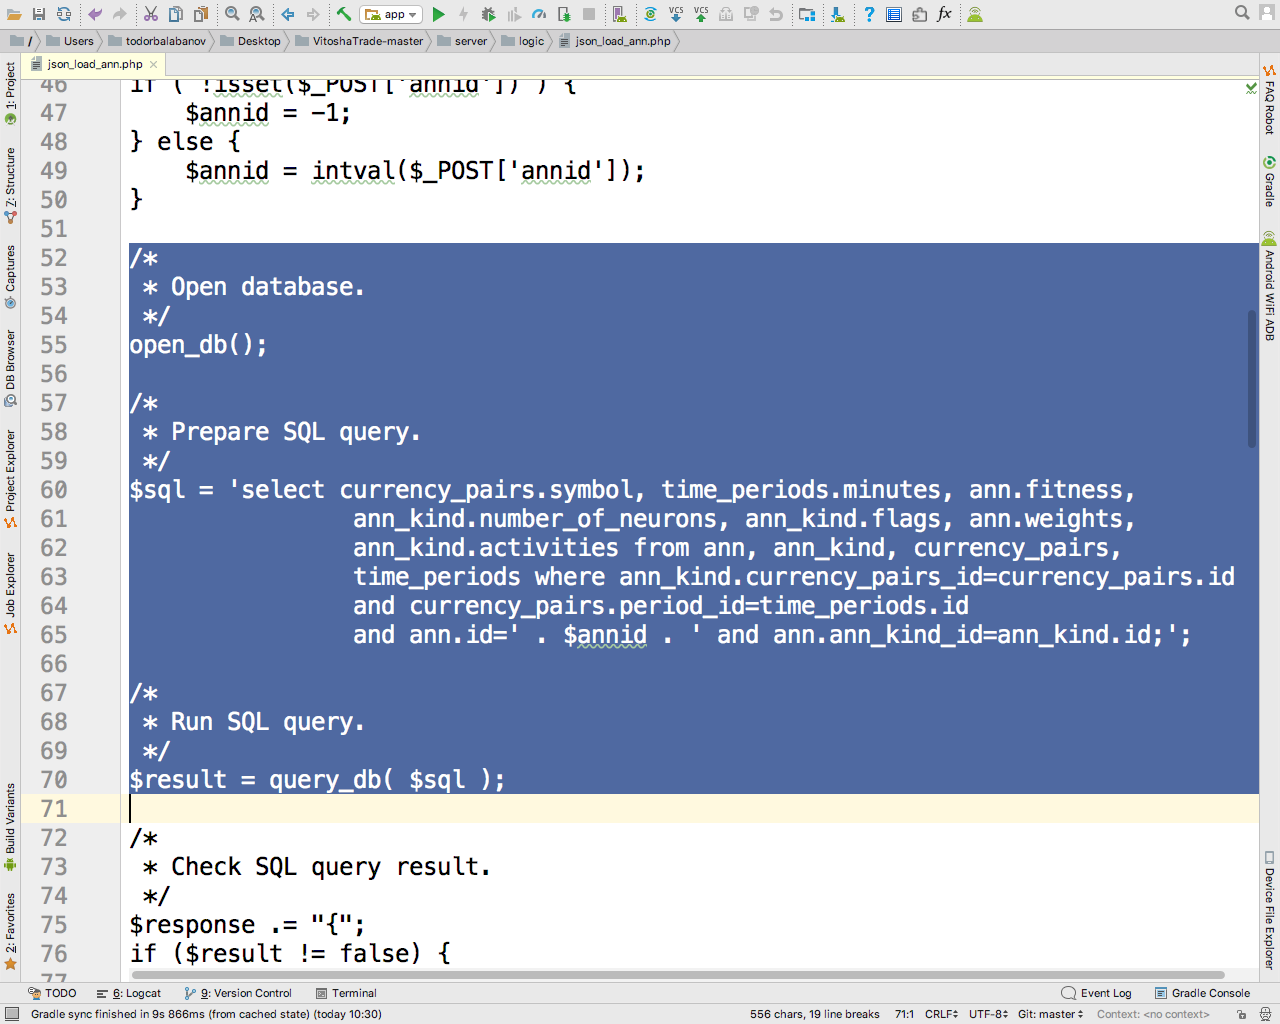
\includegraphics[height=0.45\pdfpageheight]{pic0116}
\caption{Query to retrieve instance by identifier}
\label{fig:pic0116}
\end{figure}
\FloatBarrier

This is followed by opening a connection to the database, constructing a query (good practice calls for a stored function call), and executing the query (Fig. \ref{fig:pic0116}).

\begin{figure}[h]
\centering
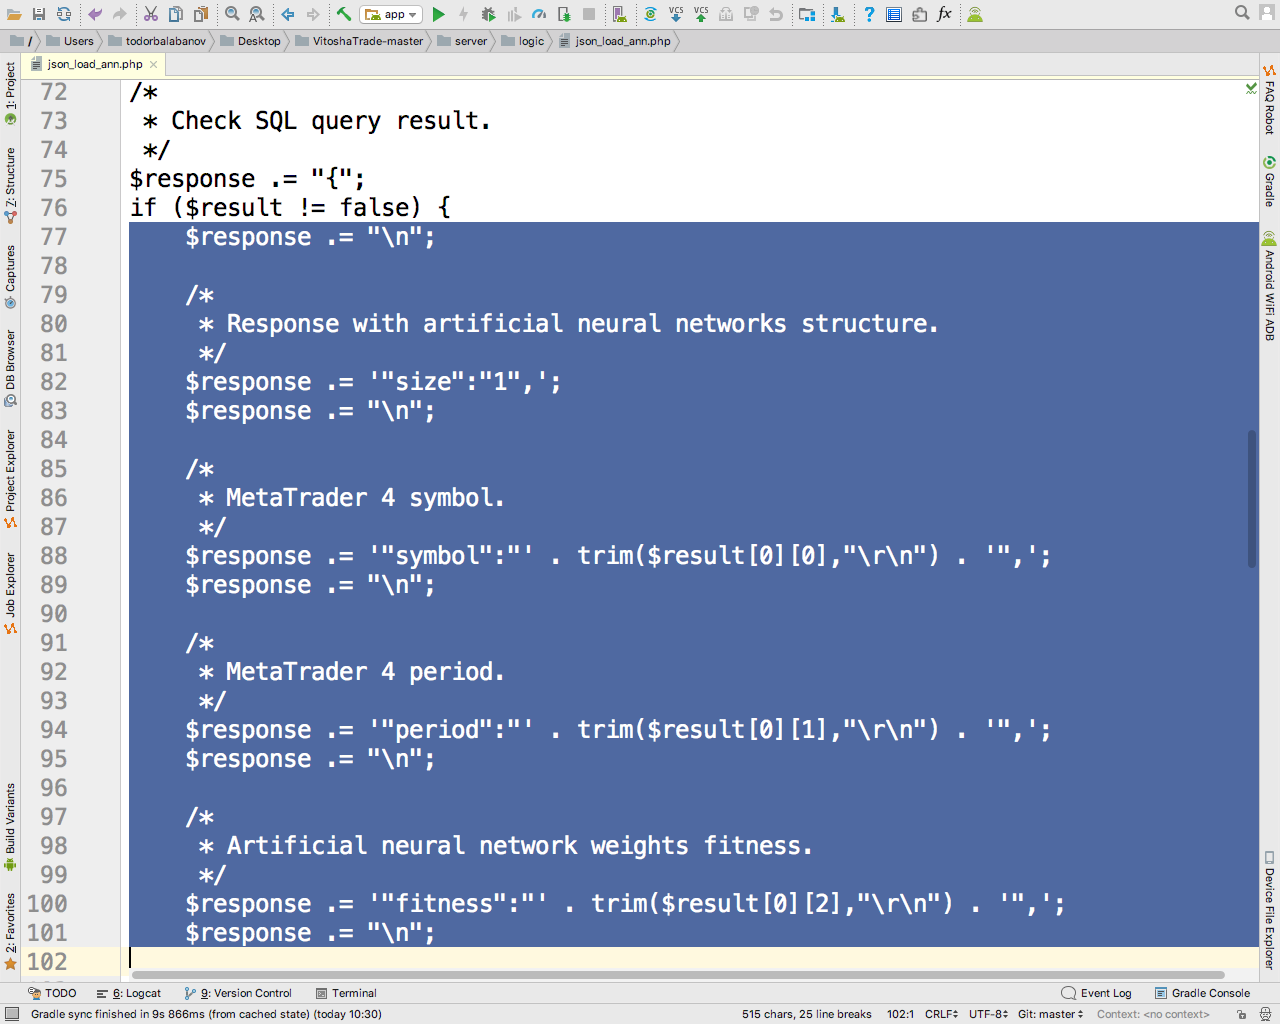
\includegraphics[height=0.45\pdfpageheight]{pic0117}
\caption{Instance availability check}
\label{fig:pic0117}
\end{figure}
\FloatBarrier

There are two possible exits from the execution of the query, depending on whether such an instance is present in the database or not. If the instance is found, it starts building a JSON message with a response to the client. The response contains a unit, per found instance, the name of the currency pair, the interval of the time series, the lifetime value of the instance, the number and types of neurons, a matrix of connections and a matrix of weights (Fig. \ref{fig:pic0117}-\ref{ fig:pic0120}).

\begin{figure}[h]
\centering
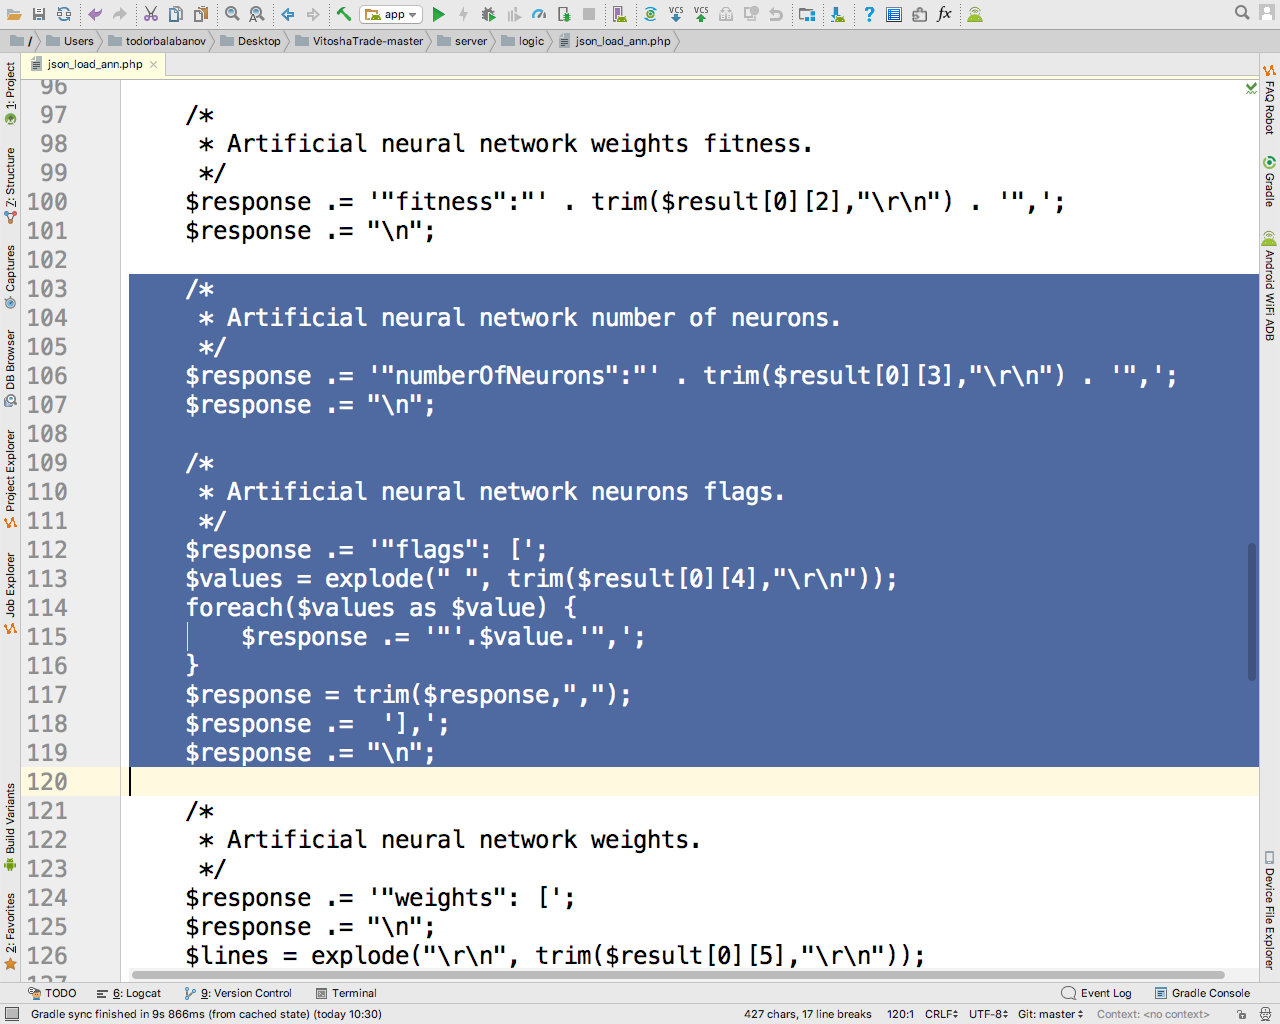
\includegraphics[height=0.45\pdfpageheight]{pic0118}
\caption{Information about neurons}
\label{fig:pic0118}
\end{figure}
\FloatBarrier

\begin{figure}[h]
\centering
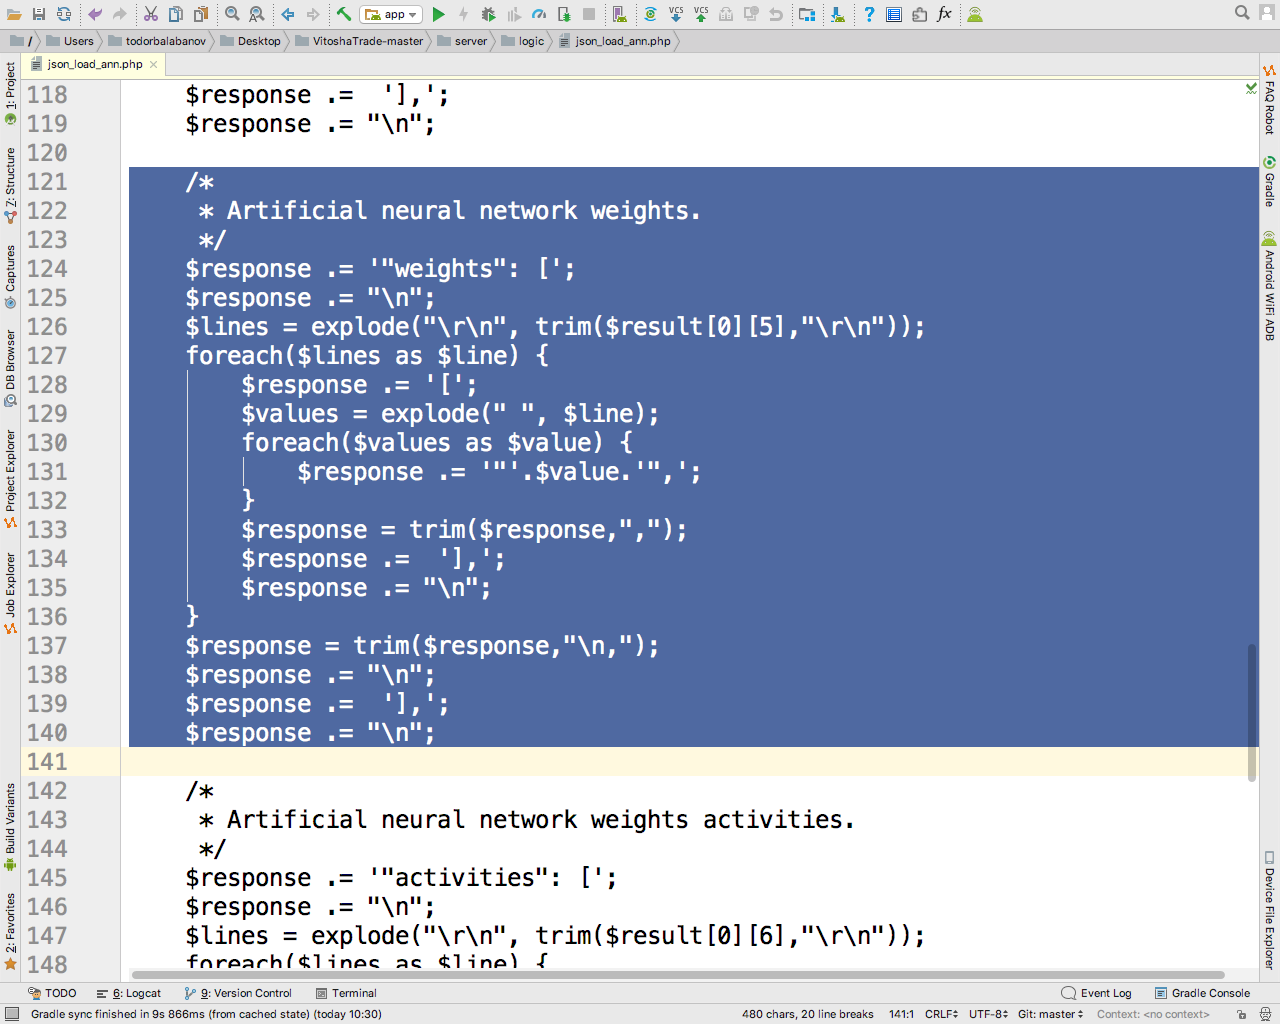
\includegraphics[height=0.45\pdfpageheight]{pic0119}
\caption{Link Information}
\label{fig:pic0119}
\end{figure}
\FloatBarrier

\begin{figure}[h]
\centering
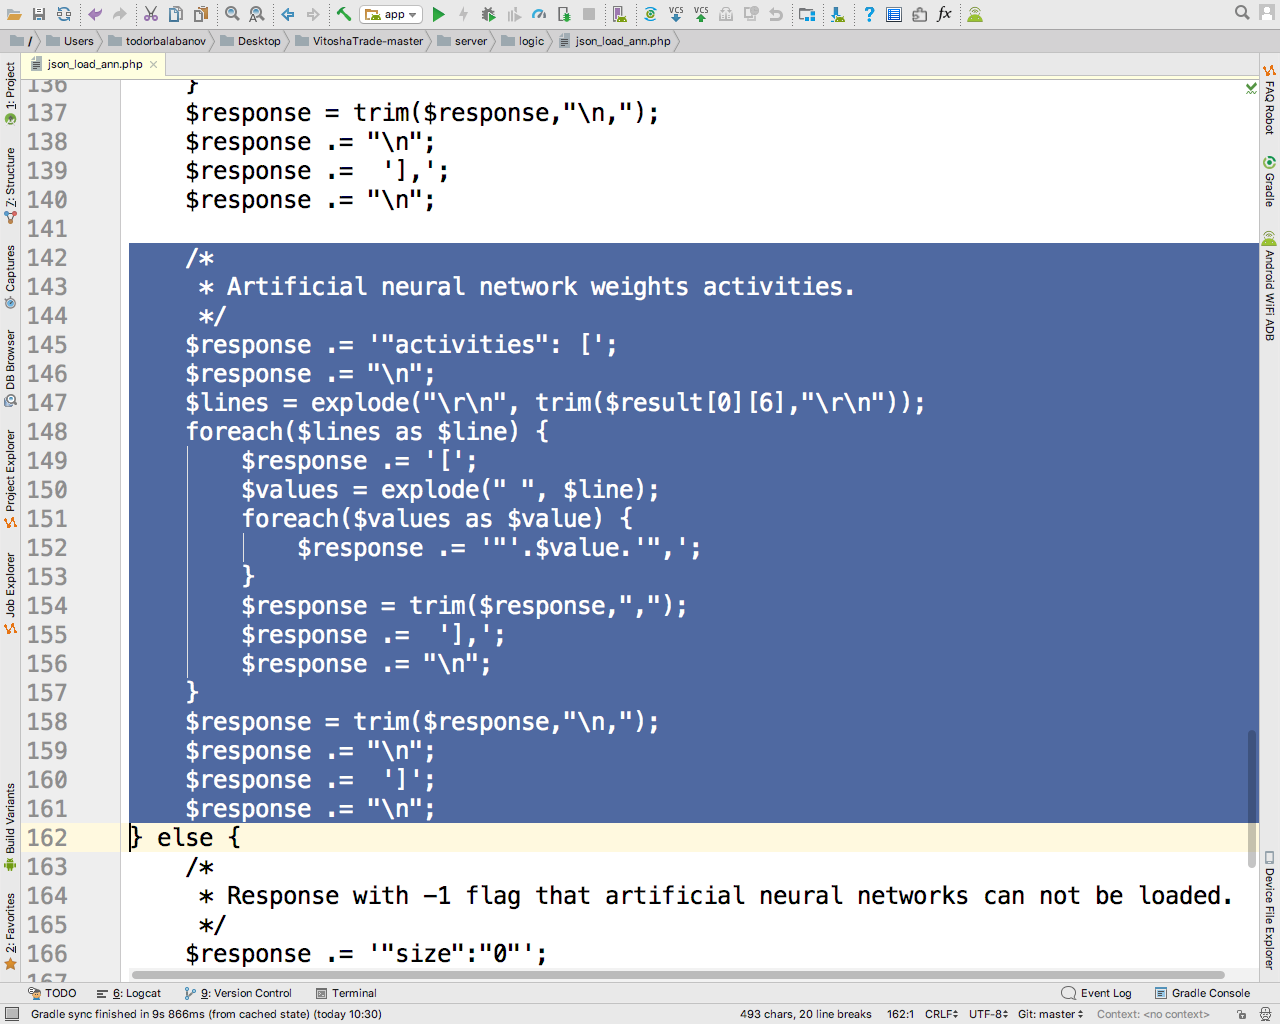
\includegraphics[height=0.45\pdfpageheight]{pic0120}
\caption{Information about weights}
\label{fig:pic0120}
\end{figure}
\FloatBarrier

In the situation when the instance is not found, a null flag is returned. In either case (discovered or not), the JSON message is completed, the database is closed, and the information is sent to the client (Fig. \ref{fig:pic0121}).

\begin{figure}[h]
\centering
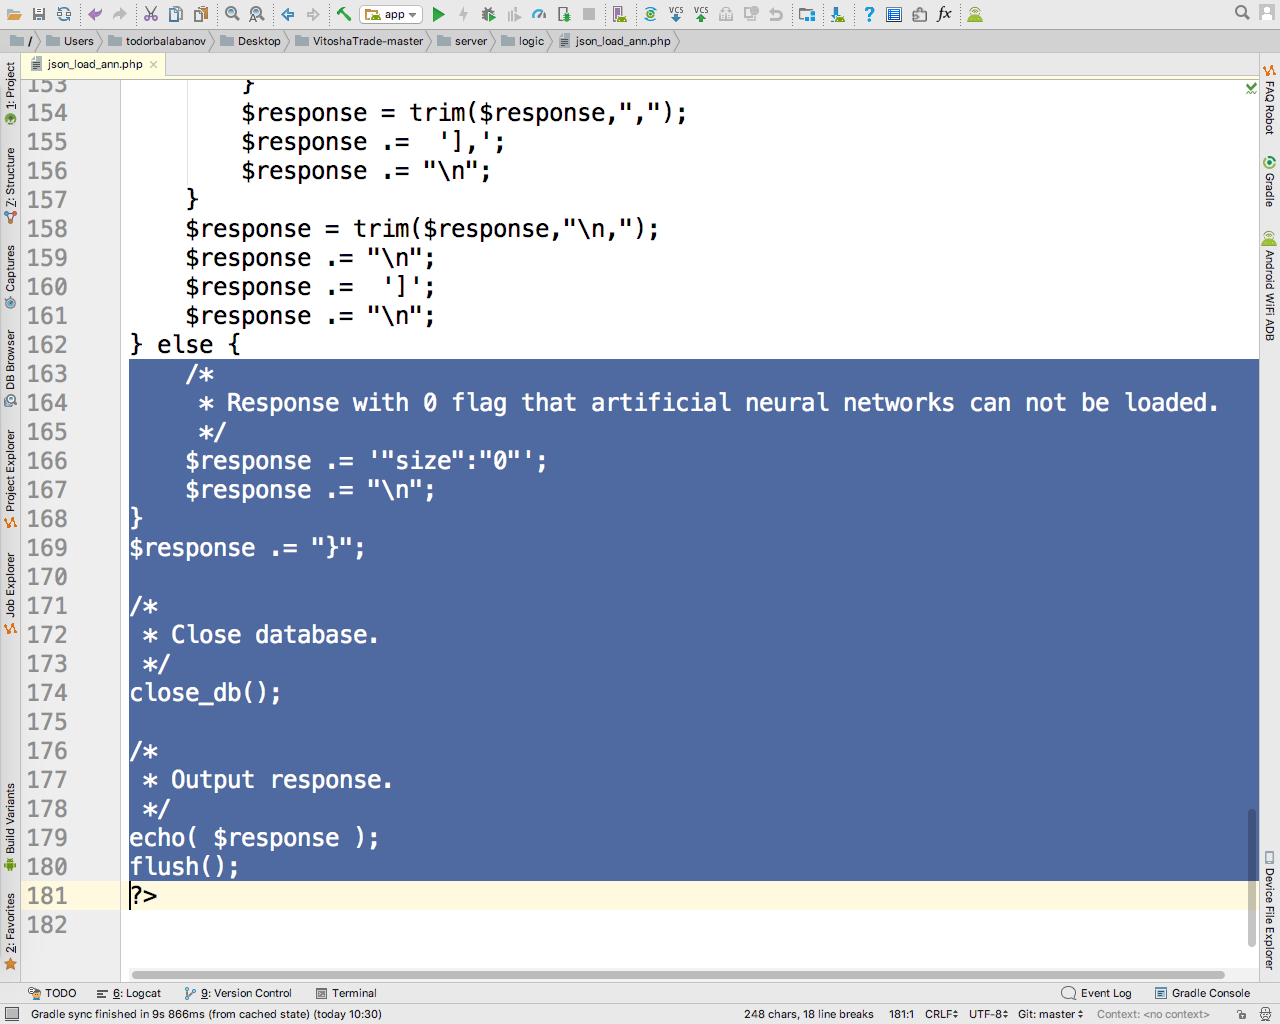
\includegraphics[height=0.45\pdfpageheight]{pic0121}
\caption{Completing the procedure for sending a response}
\label{fig:pic0121}
\end{figure}
\FloatBarrier

\subsection{Load a random grid}

When computations are performed on the principle of donated computing power, it is logical that the selection of the network to be further trained should be random. For this purpose, the server-side script selects the network in a random manner.

\begin{figure}[h]
\centering
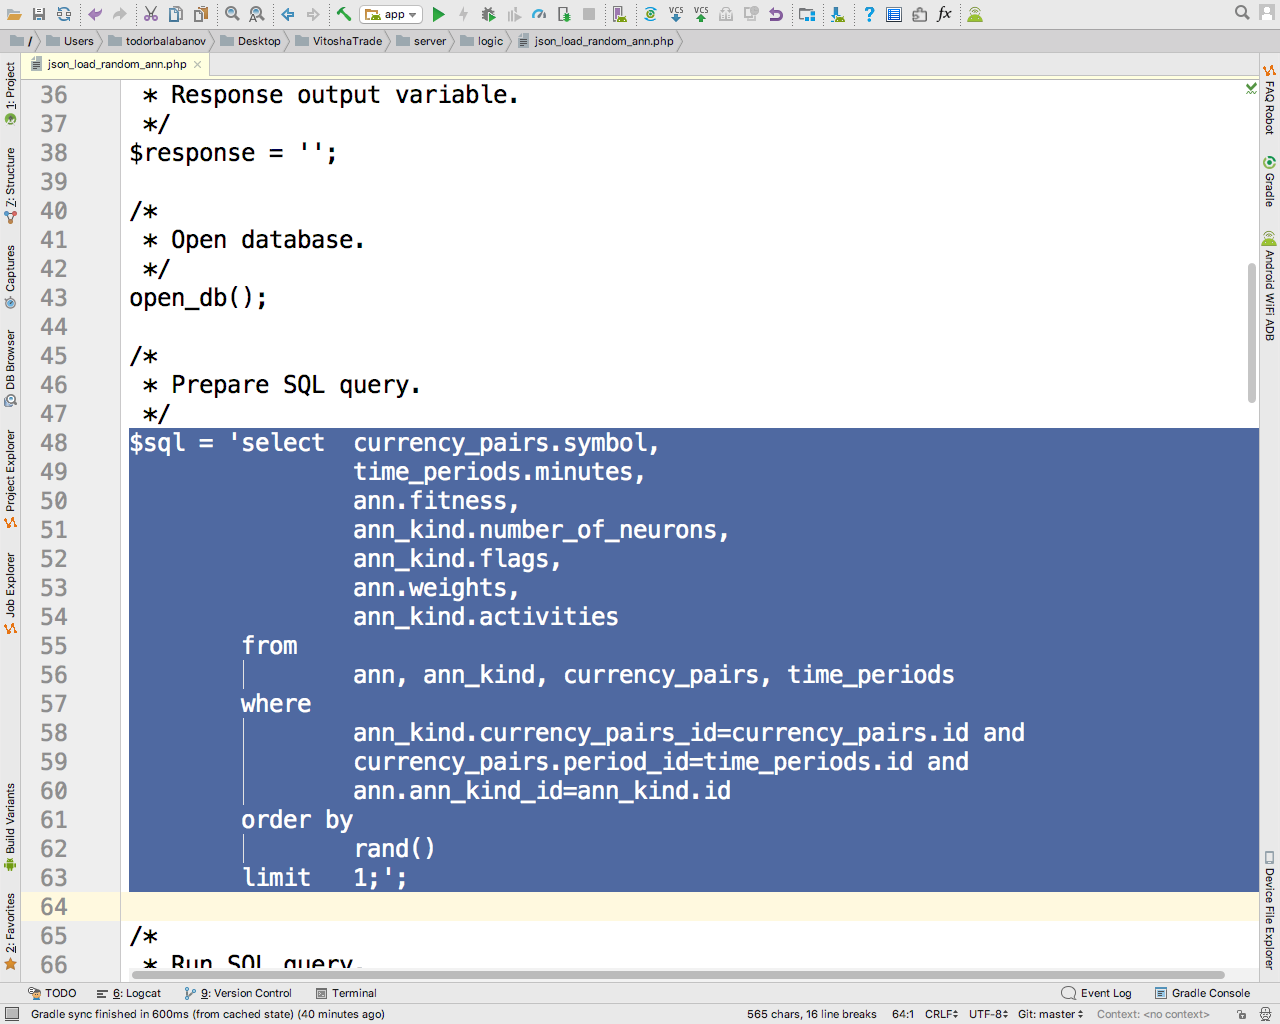
\includegraphics[height=0.45\pdfpageheight]{pic0157}
\caption{Request to Load Random Grid}
\label{fig:pic0157}
\end{figure}
\FloatBarrier

The only difference between loading a grid by identifiers and a random grid is in the SQL query that is executed by MySQL (Fig. \ref{fig:pic0157}).

\subsection{Loading the best vitality from the global population}

One of the main criteria by which client applications decide whether to report the results they find is the best liveness value in the global population (the population that is stored on the server). The script responsible for this check also includes the database module and performs a series of checks on the input parameters.

\begin{figure}[h]
\centering
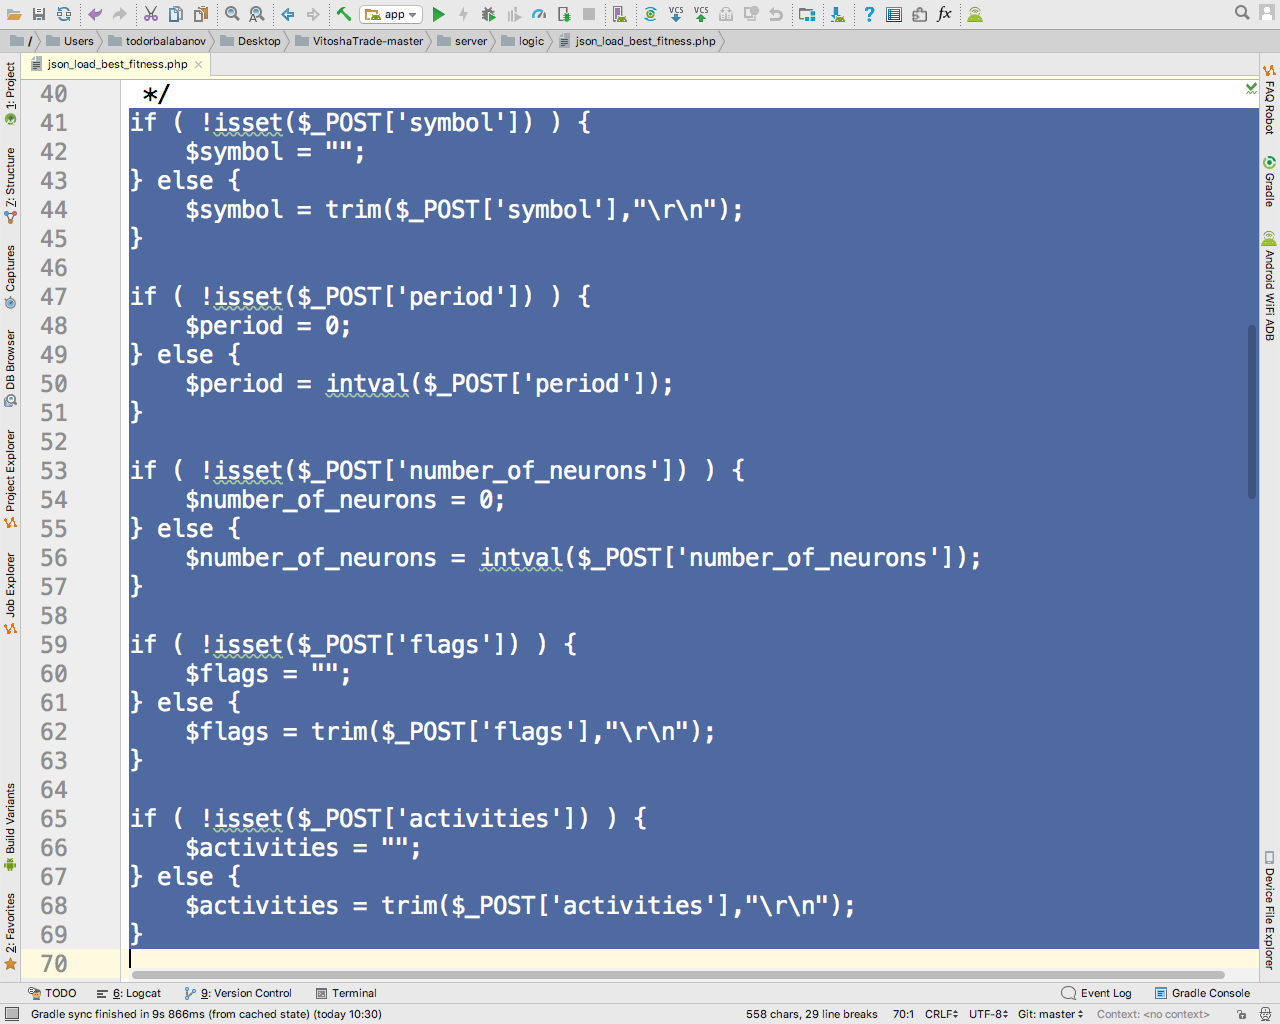
\includegraphics[height=0.45\pdfpageheight]{pic0122}
\caption{Input parameters for a specific neural network topology}
\label{fig:pic0122}
\end{figure}
\FloatBarrier

The name of the currency pair, the period of the time series, the number and types of neurons, as well as the connections between them are checked (Fig. \ref{fig:pic0122}).

\begin{figure}[h]
\centering
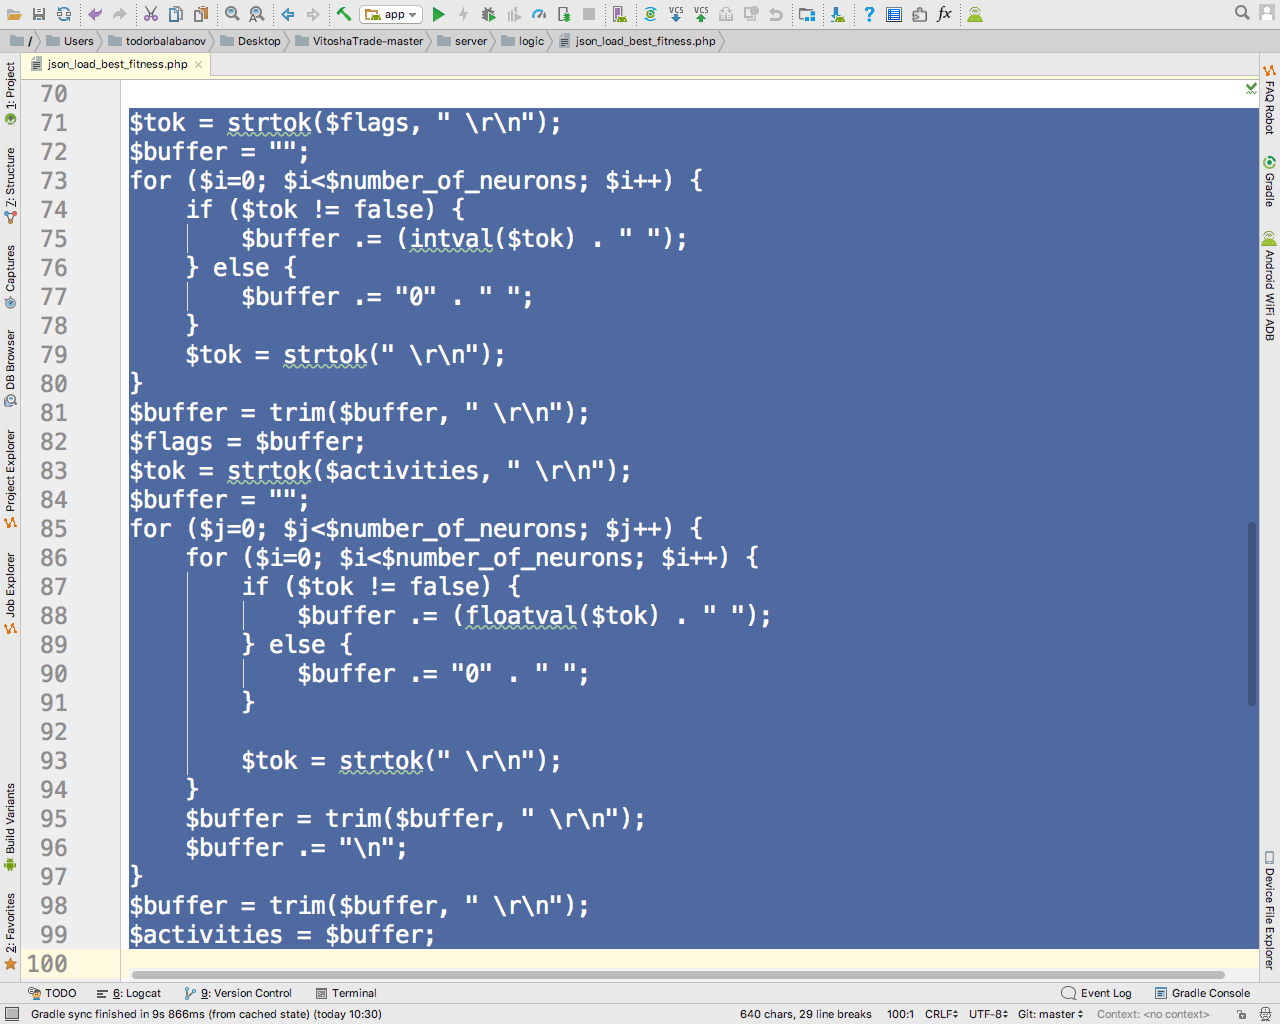
\includegraphics[height=0.45\pdfpageheight]{pic0123}
\caption{Neuron flags and connections between them}
\label{fig:pic0123}
\end{figure}
\FloatBarrier

Since the neuron types are represented as an array, and the connections between the neurons themselves in an adjacency matrix, checking them requires a bit more complex processing in loops (Fig. \ref{fig:pic0123}).

\begin{figure}[h]
\centering
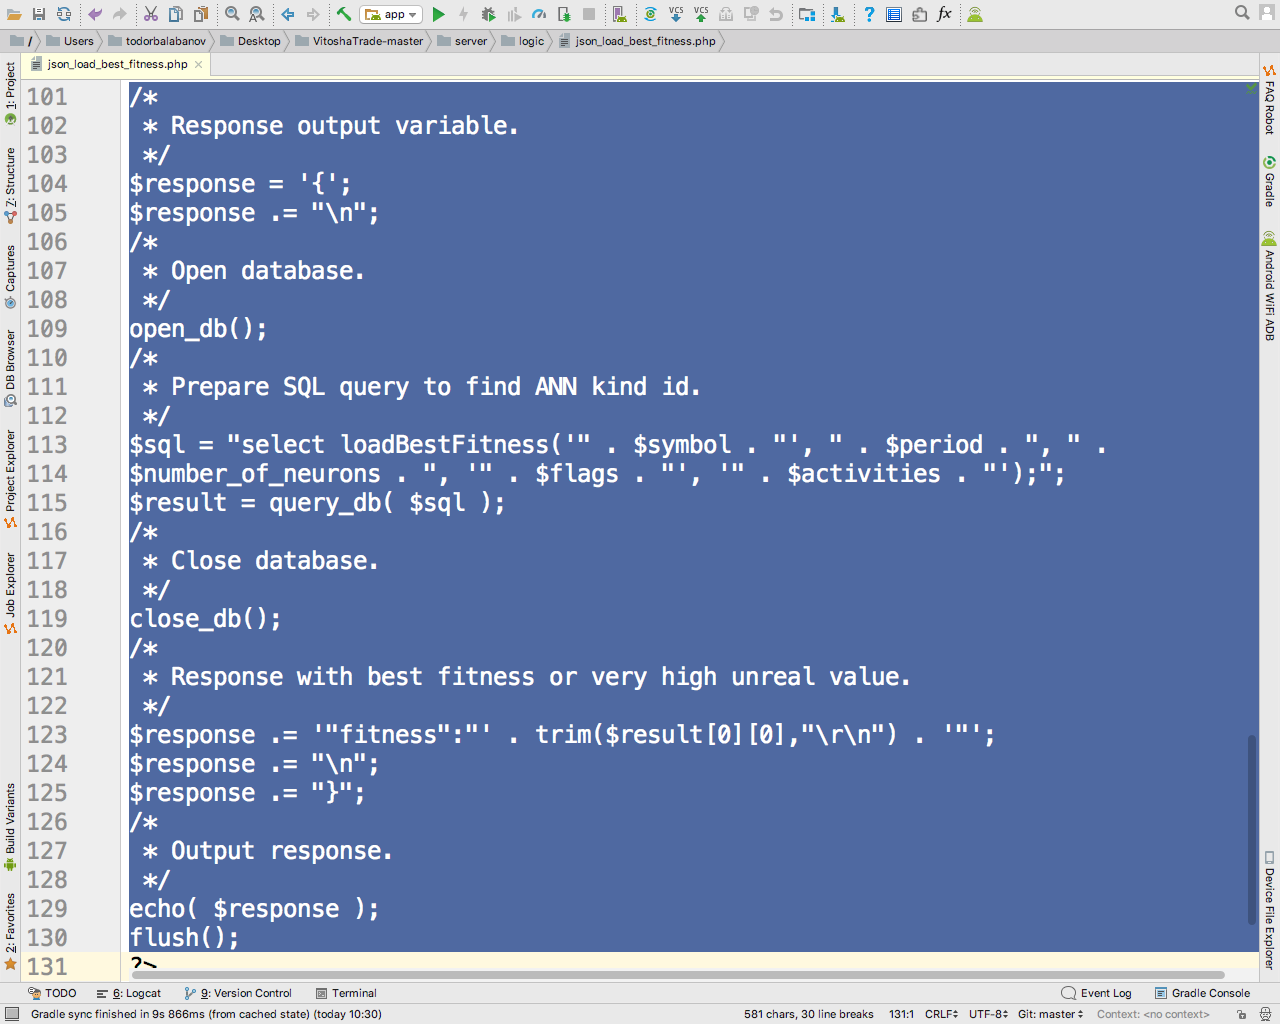
\includegraphics[height=0.45\pdfpageheight]{pic0124}
\caption{Best Vitality Request}
\label{fig:pic0124}
\end{figure}
\FloatBarrier

This is followed by opening the database connection, executing the best liveness detection stored function, closing the database, and sending a JSON packed response to the client (Fig. \ref{fig:pic0124}).

\subsection{Loading number of neurons by ID}

When working with instances of artificial neural networks, it is essential to inquire about the number of neurons in the network.

\begin{figure}[h]
\centering
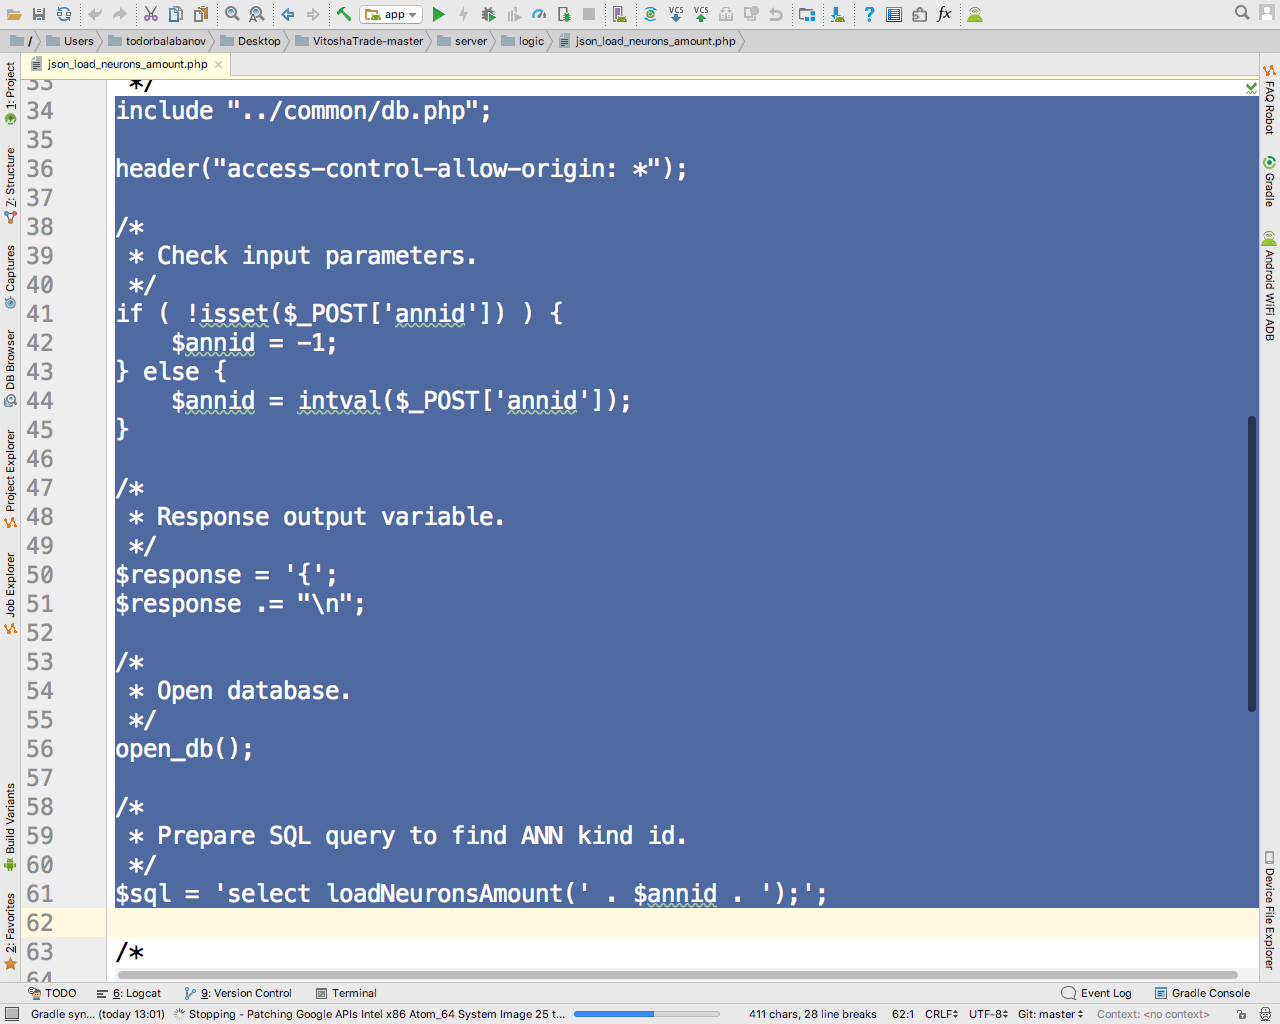
\includegraphics[height=0.45\pdfpageheight]{pic0125}
\caption{Determining the number of neurons by network ID}
\label{fig:pic0125}
\end{figure}
\FloatBarrier

The procedure again includes the database module, checking the input parameter for an instance ID, opening a connection to the database, and running a stored function (Fig. \ref{fig:pic0125}).

\begin{figure}[h]
\centering
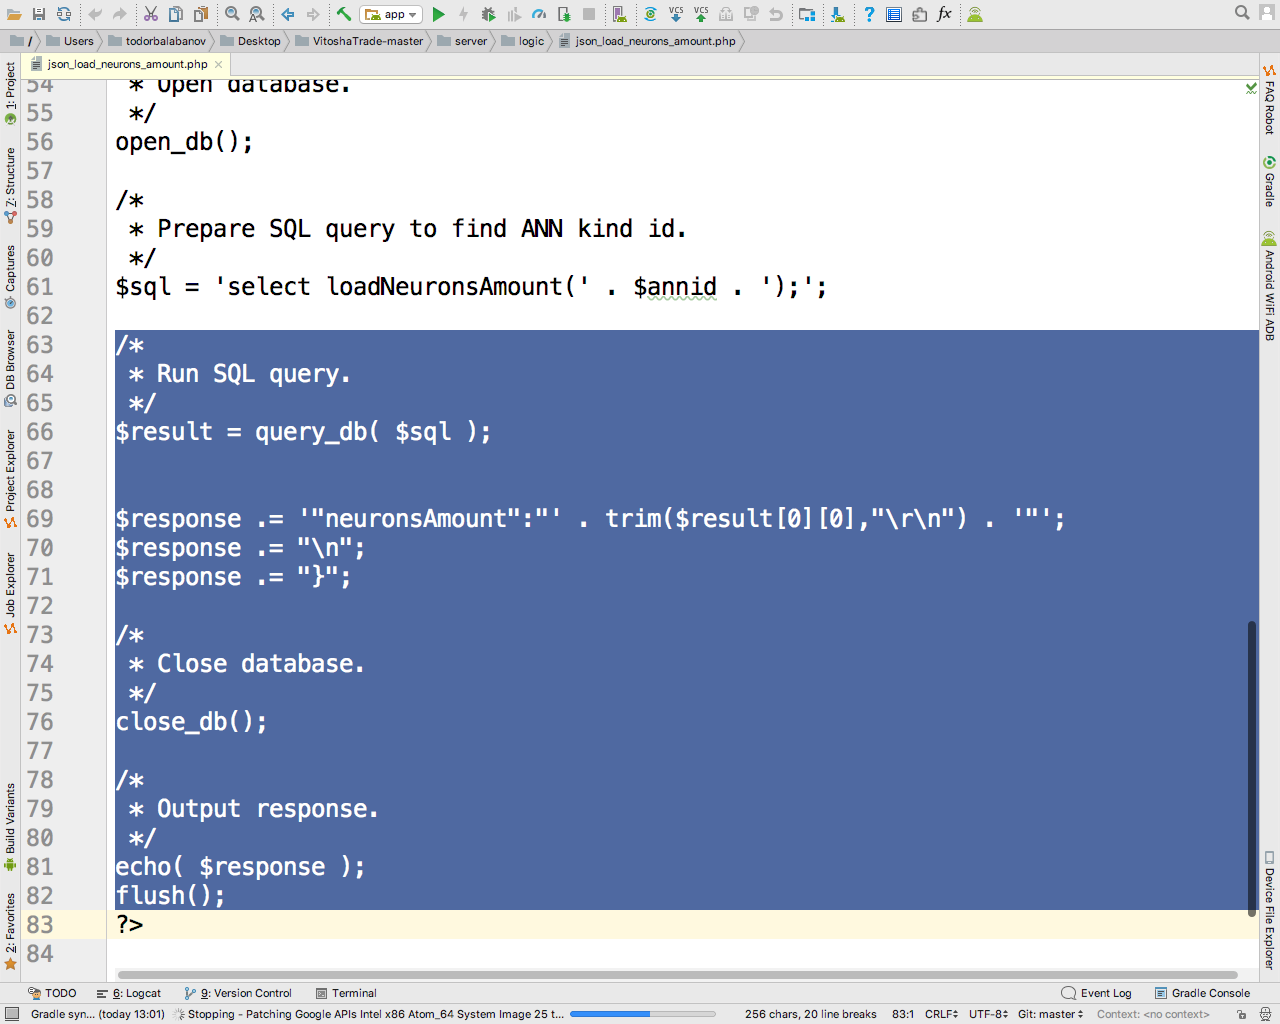
\includegraphics[height=0.45\pdfpageheight]{pic0126}
\caption{Response to customer}
\label{fig:pic0126}
\end{figure}
\FloatBarrier

The result of the stored function is packed into a JSON message and sent to the client (Fig. \ref{fig:pic0126}).

\subsection{Loading Training Set by Currency Pair Information}

For the training of each artificial neural network, a training set is used, which is different according to the name of the currency pair and the time interval of the order.

\begin{figure}[h]
\centering
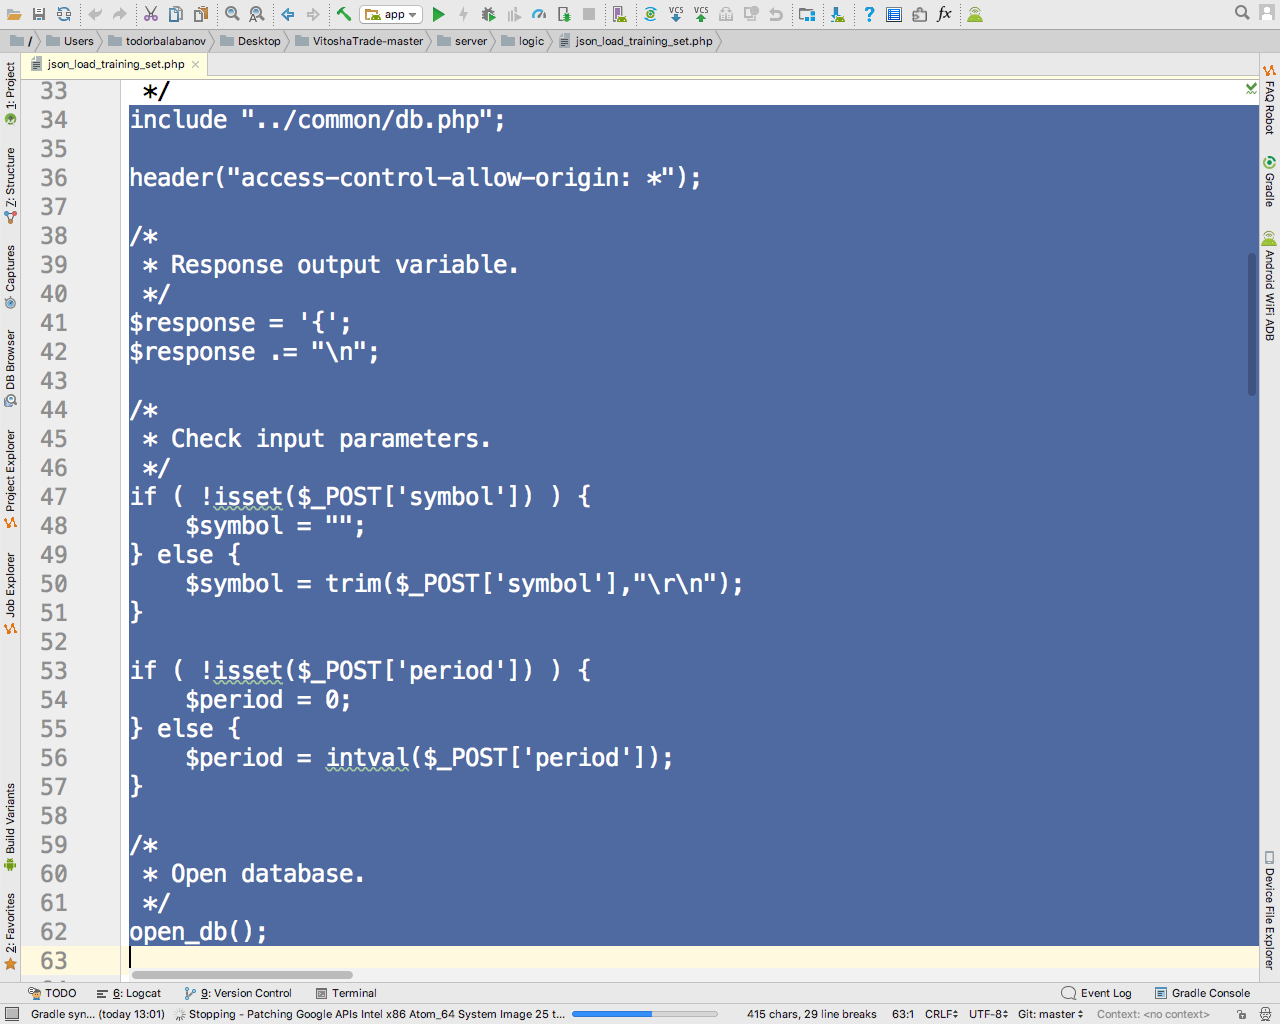
\includegraphics[height=0.45\pdfpageheight]{pic0127}
\caption{Checking input parameters}
\label{fig:pic0127}
\end{figure}
\FloatBarrier

Booting begins in the classic way by turning on the database module, checking input information, and opening a connection to the database (Fig. \ref{fig:pic0127}).

\begin{figure}[h]
\centering
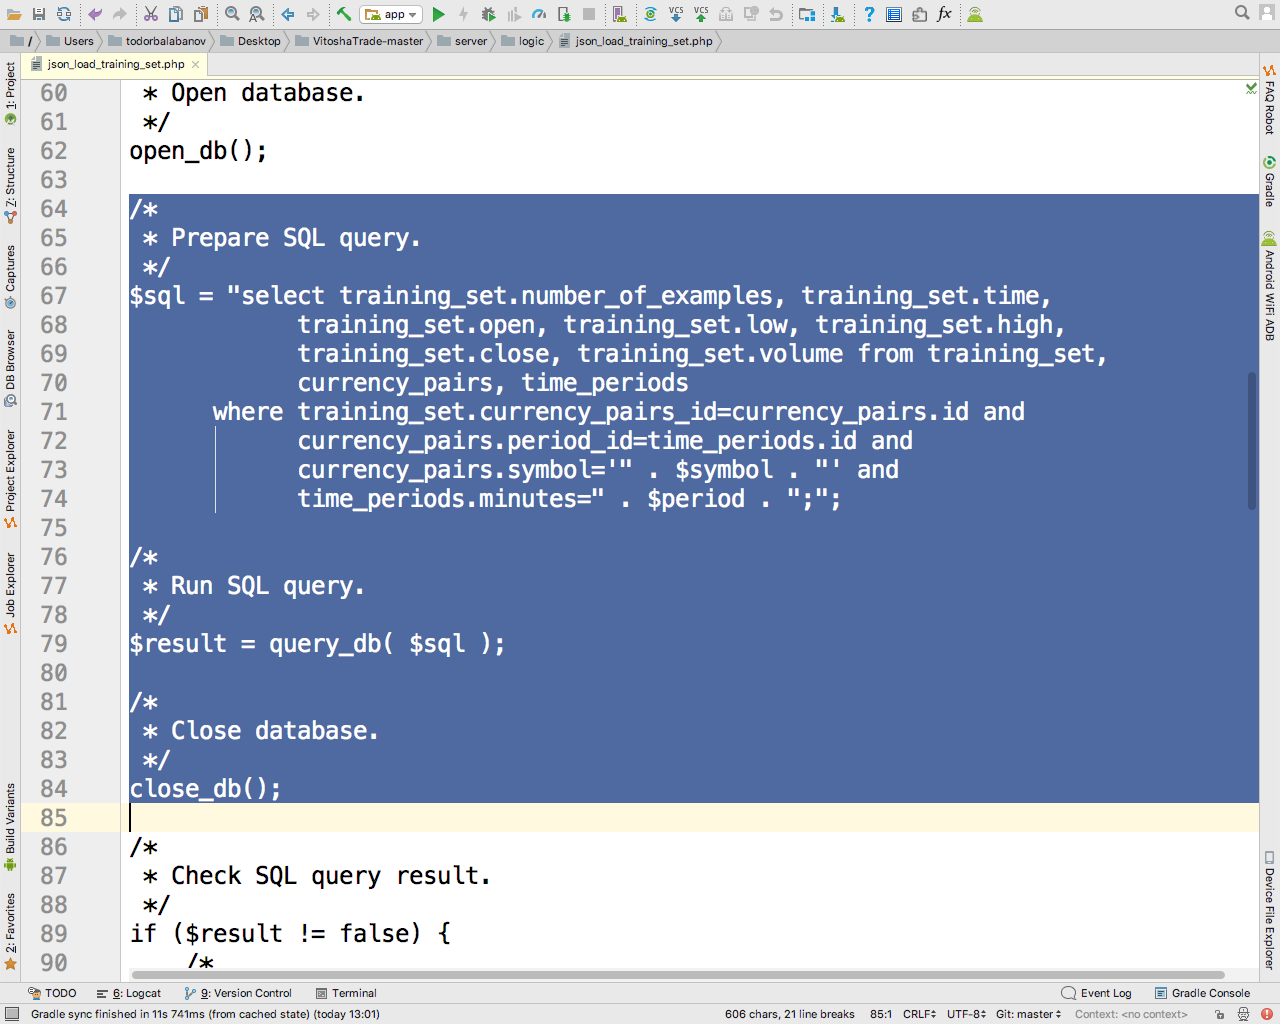
\includegraphics[height=0.45\pdfpageheight]{pic0128}
\caption{Request for training set}
\label{fig:pic0128}
\end{figure}
\FloatBarrier

Next comes a query, retrieving the result, and closing the database connection (Fig. \ref{fig:pic0128}). Although not done, good layer separation style suggests calling a stored function instead of a query.

\begin{figure}[h]
\centering
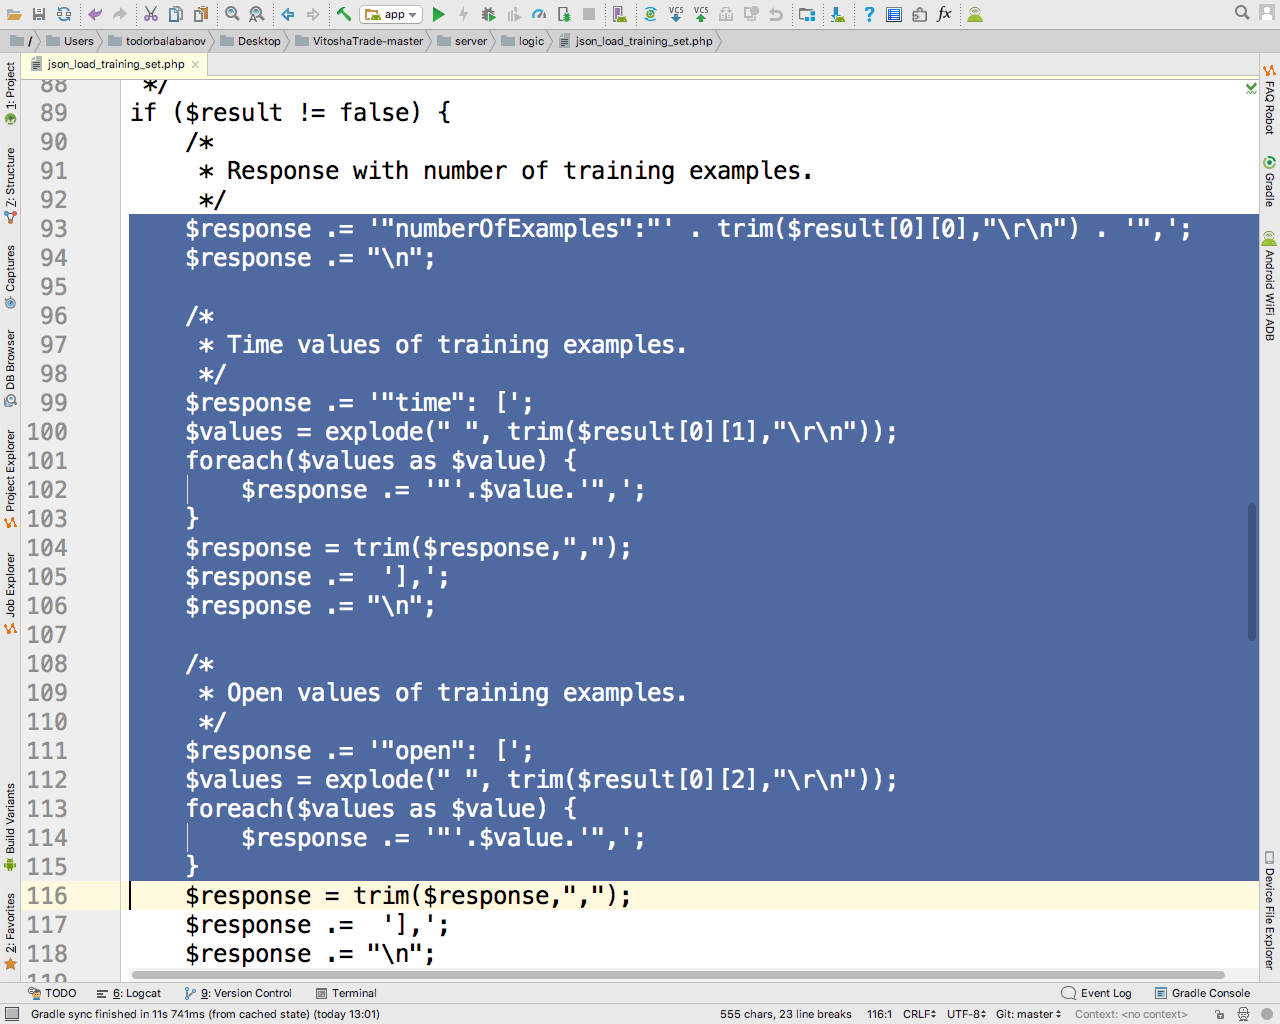
\includegraphics[height=0.45\pdfpageheight]{pic0129}
\caption{Number of examples, timestamps and opening levels}
\label{fig:pic0129}
\end{figure}
\FloatBarrier

\begin{figure}[h]
\centering
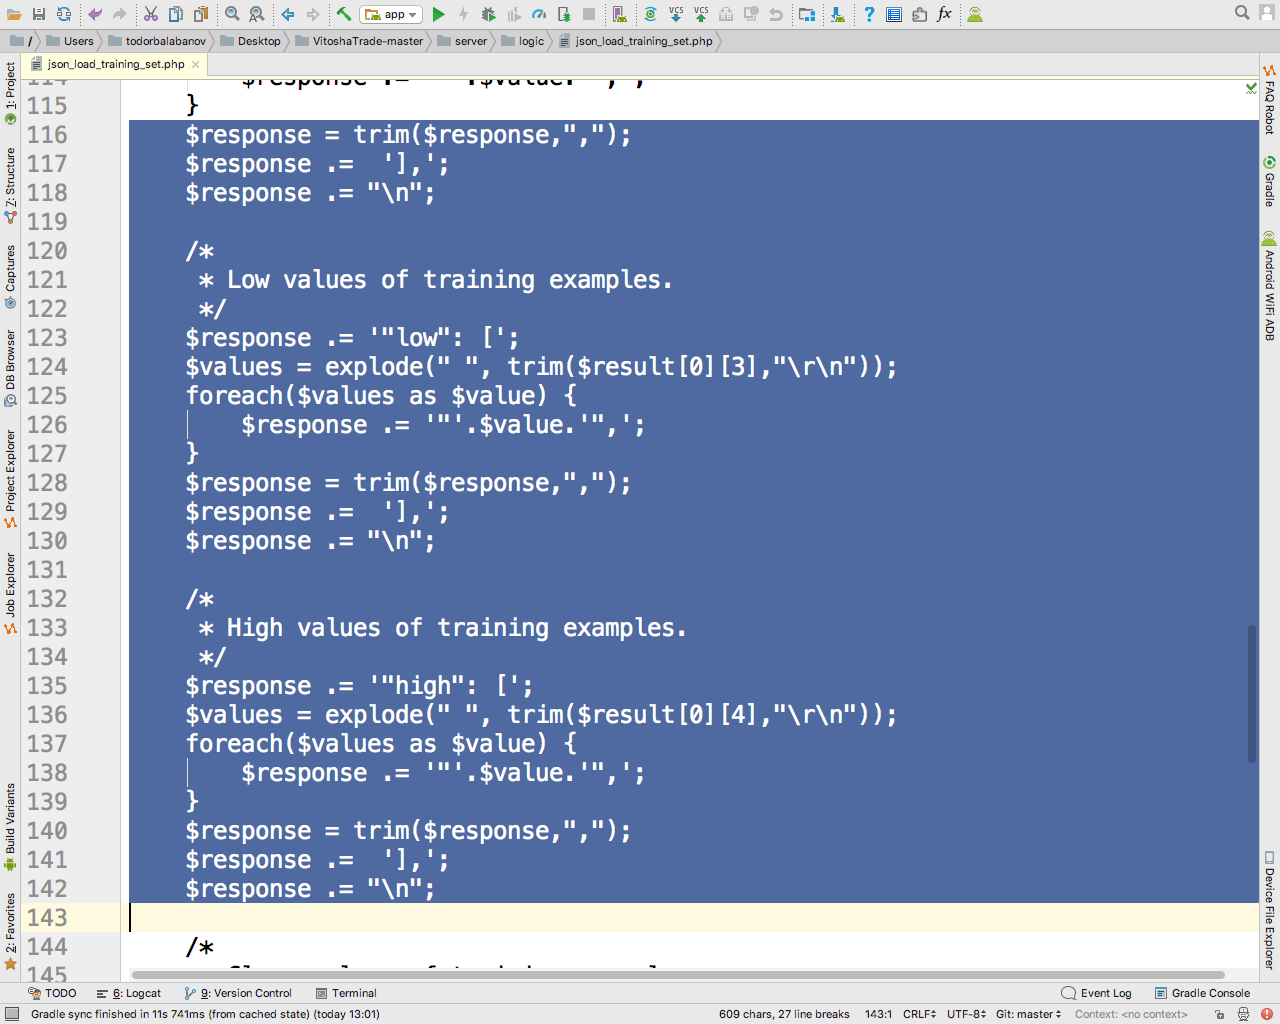
\includegraphics[height=0.45\pdfpageheight]{pic0130}
\caption{Lowest and highest value achieved}
\label{fig:pic0130}
\end{figure}
\FloatBarrier

\begin{figure}[h]
\centering
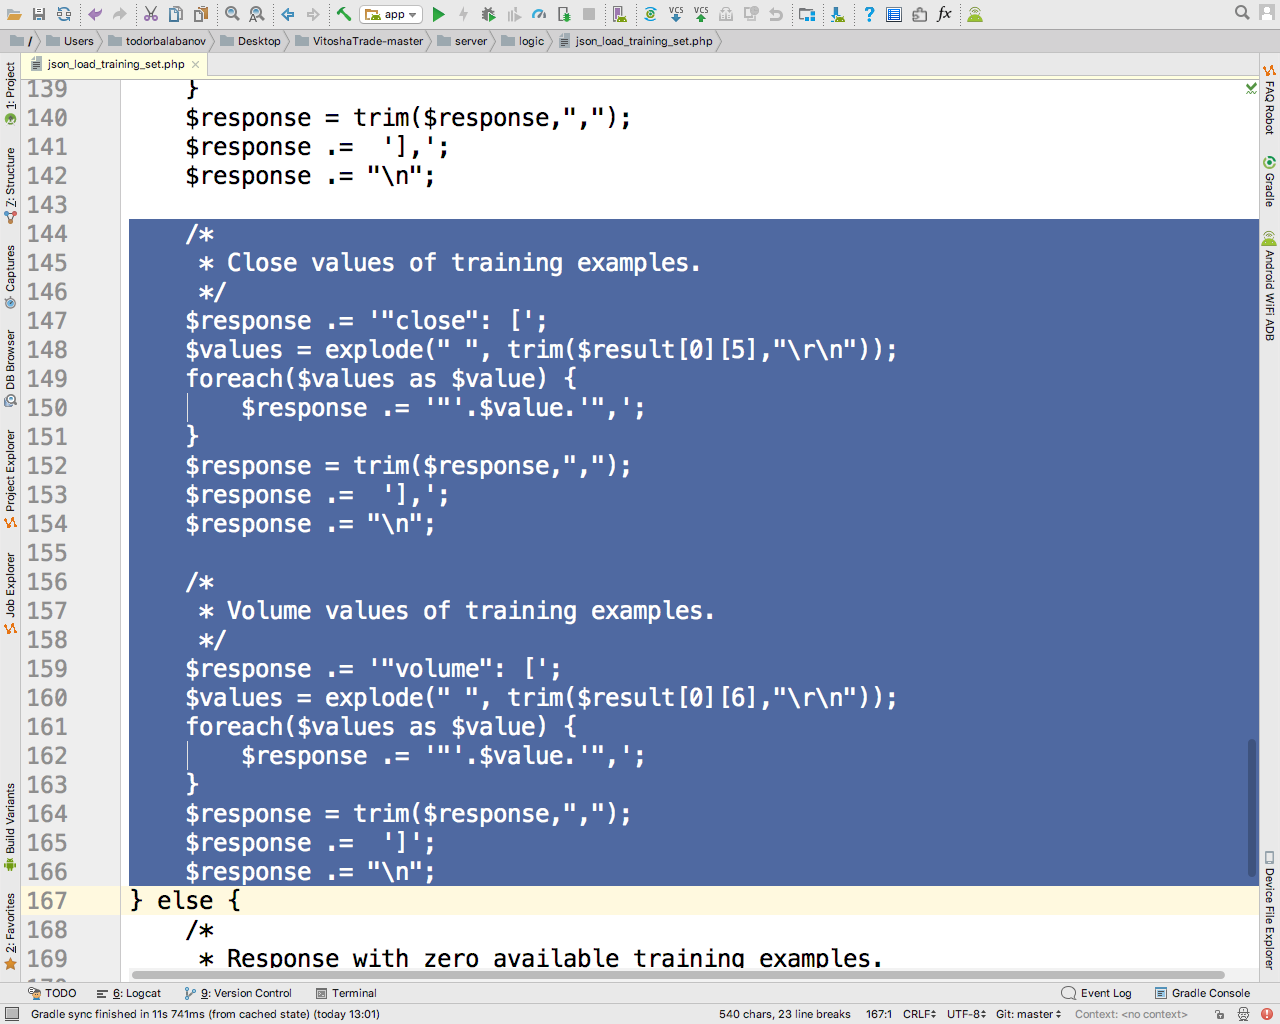
\includegraphics[height=0.45\pdfpageheight]{pic0131}
\caption{Closing levels and traded volume}
\label{fig:pic0131}
\end{figure}
\FloatBarrier

If a training set is found for the specified currency pair and time interval, then the time series values are packed and sent to the client (Fig. \ref{fig:pic0129}-\ref{fig:pic0131}).

\begin{figure}[h]
\centering
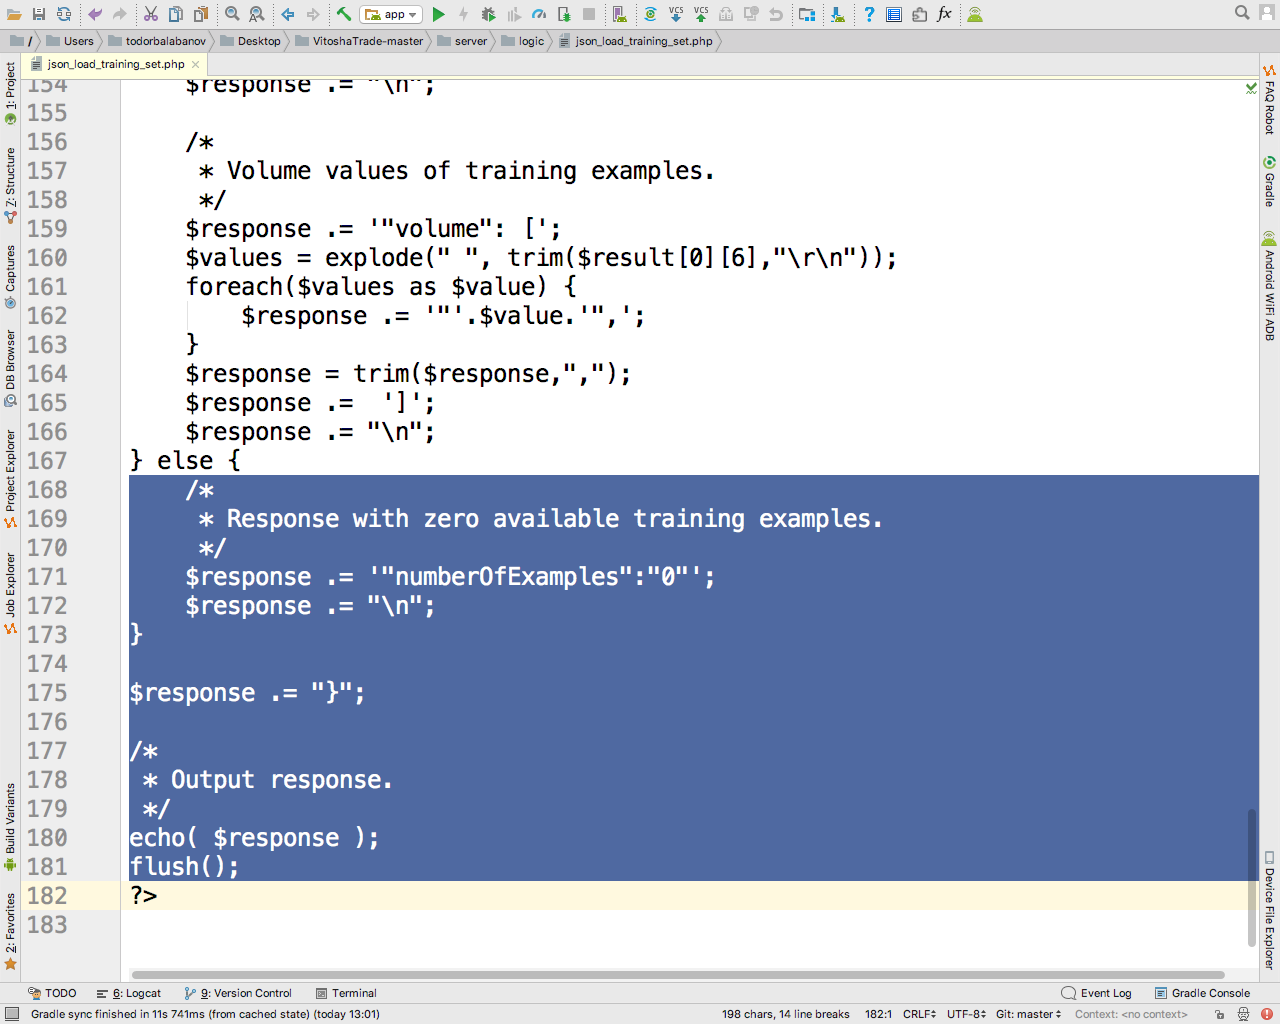
\includegraphics[height=0.45\pdfpageheight]{pic0132}
\caption{Send response to client}
\label{fig:pic0132}
\end{figure}
\FloatBarrier

If no training set is found, a message of zero size is sent for the data. Regardless of whether a set is found or not, the JSON message is sent to the client (Fig \ref{fig:pic0132}).

\subsection{Load number of instances by identifier or currency pair information}

To select a subset of the global population, it is necessary to know how many instances are present in the database by a given instance identifier or currency pair name with a period.

\begin{figure}[h]
\centering
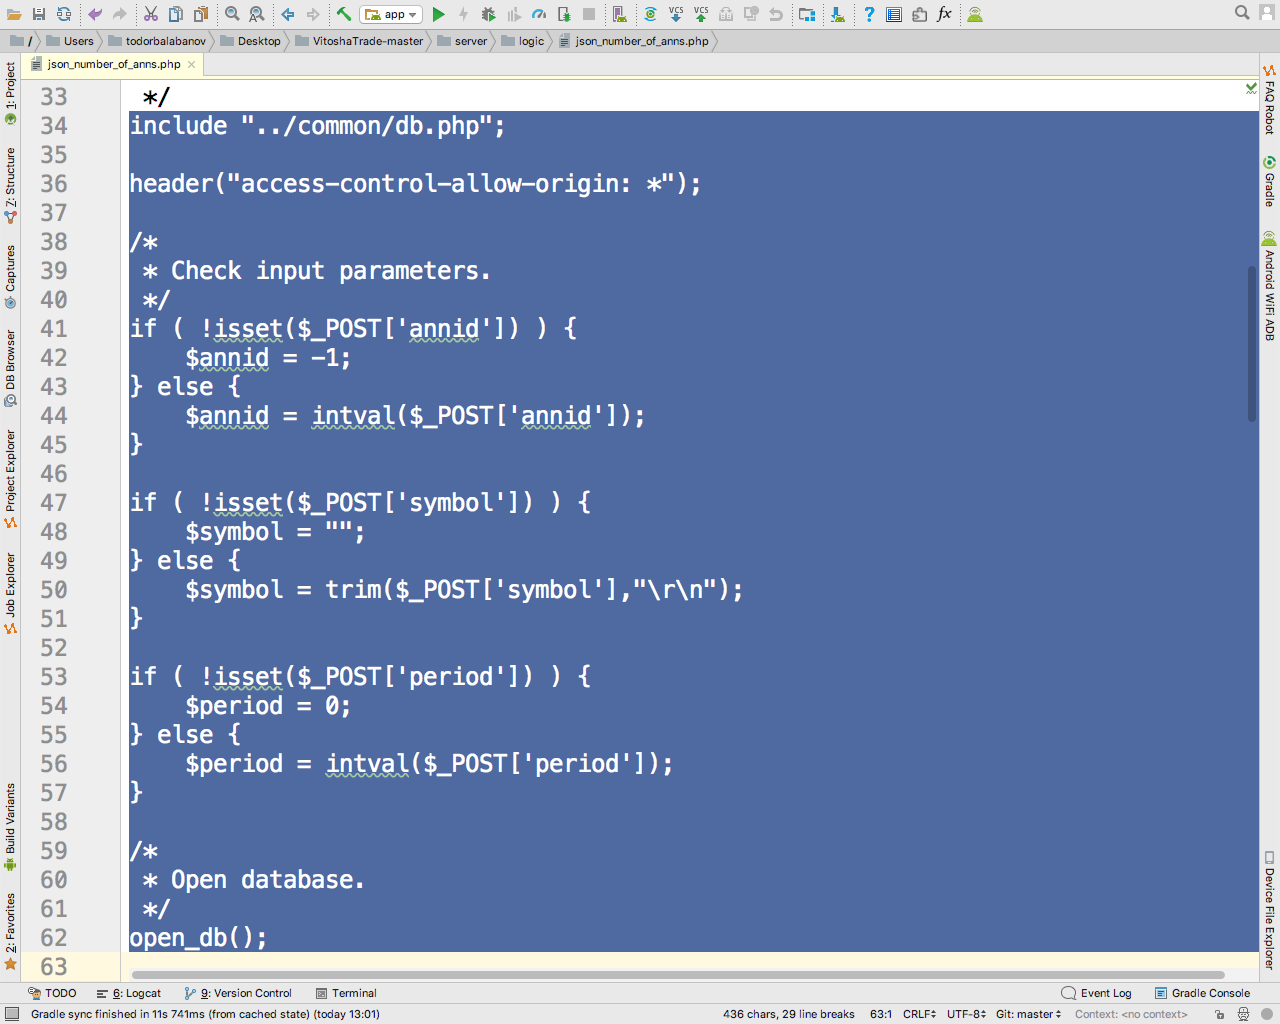
\includegraphics[height=0.45\pdfpageheight]{pic0133}
\caption{Validation of input arguments}
\label{fig:pic0133}
\end{figure}
\FloatBarrier

The check again begins by turning on the database module, checking the input arguments, and opening a connection to the database (Fig. \ref{fig:pic0133}).

\begin{figure}[h]
\centering
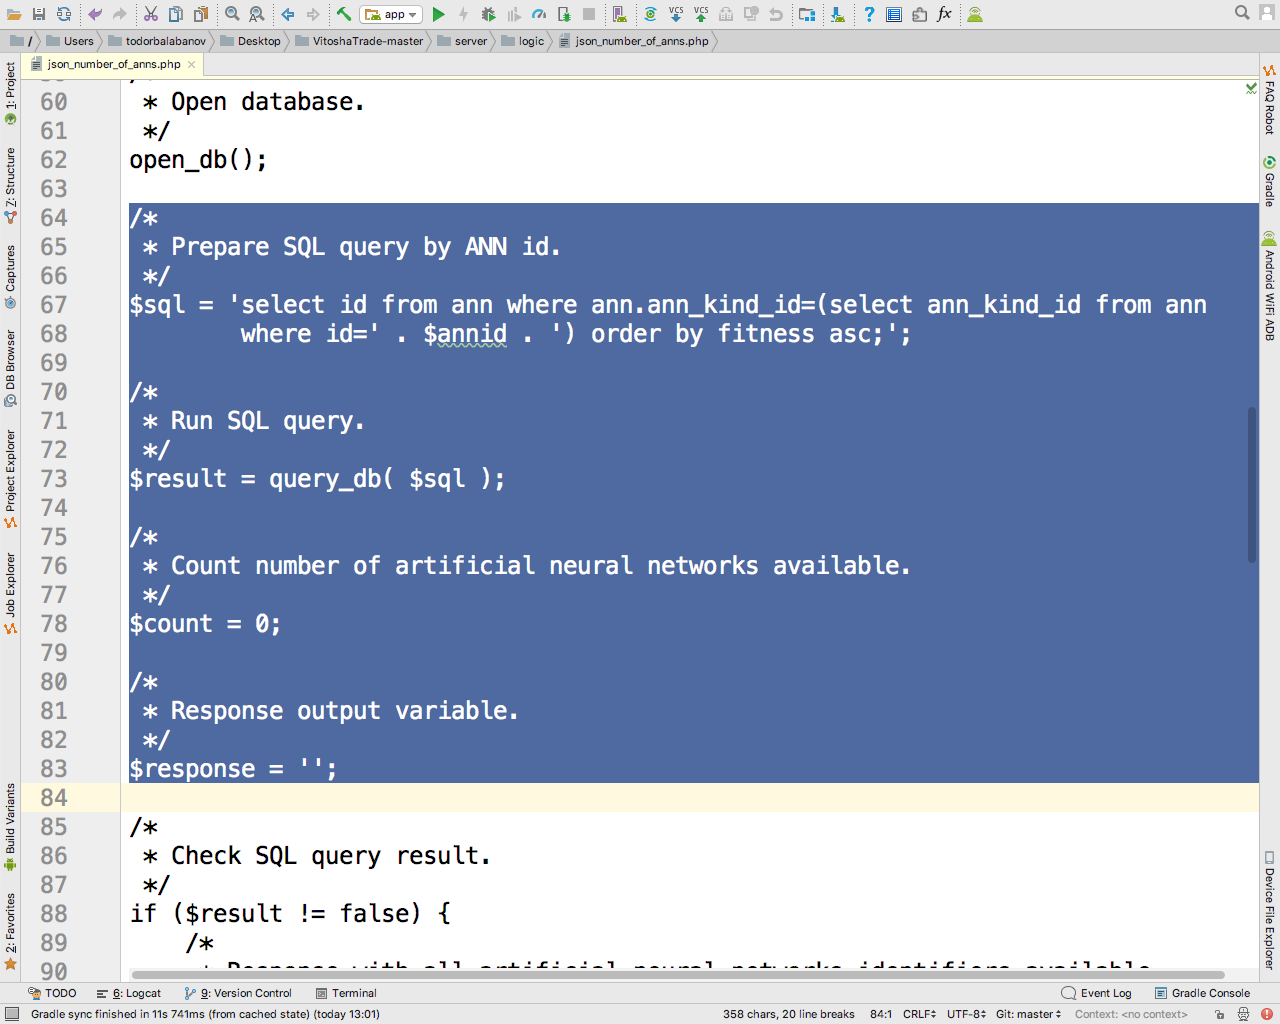
\includegraphics[height=0.45\pdfpageheight]{pic0134}
\caption{Instances of the submitted identifier type}
\label{fig:pic0134}
\end{figure}
\FloatBarrier

First, the instances that are of the type of the submitted identifier are listed (Fig. \ref{fig:pic0134}).

\begin{figure}[h]
\centering
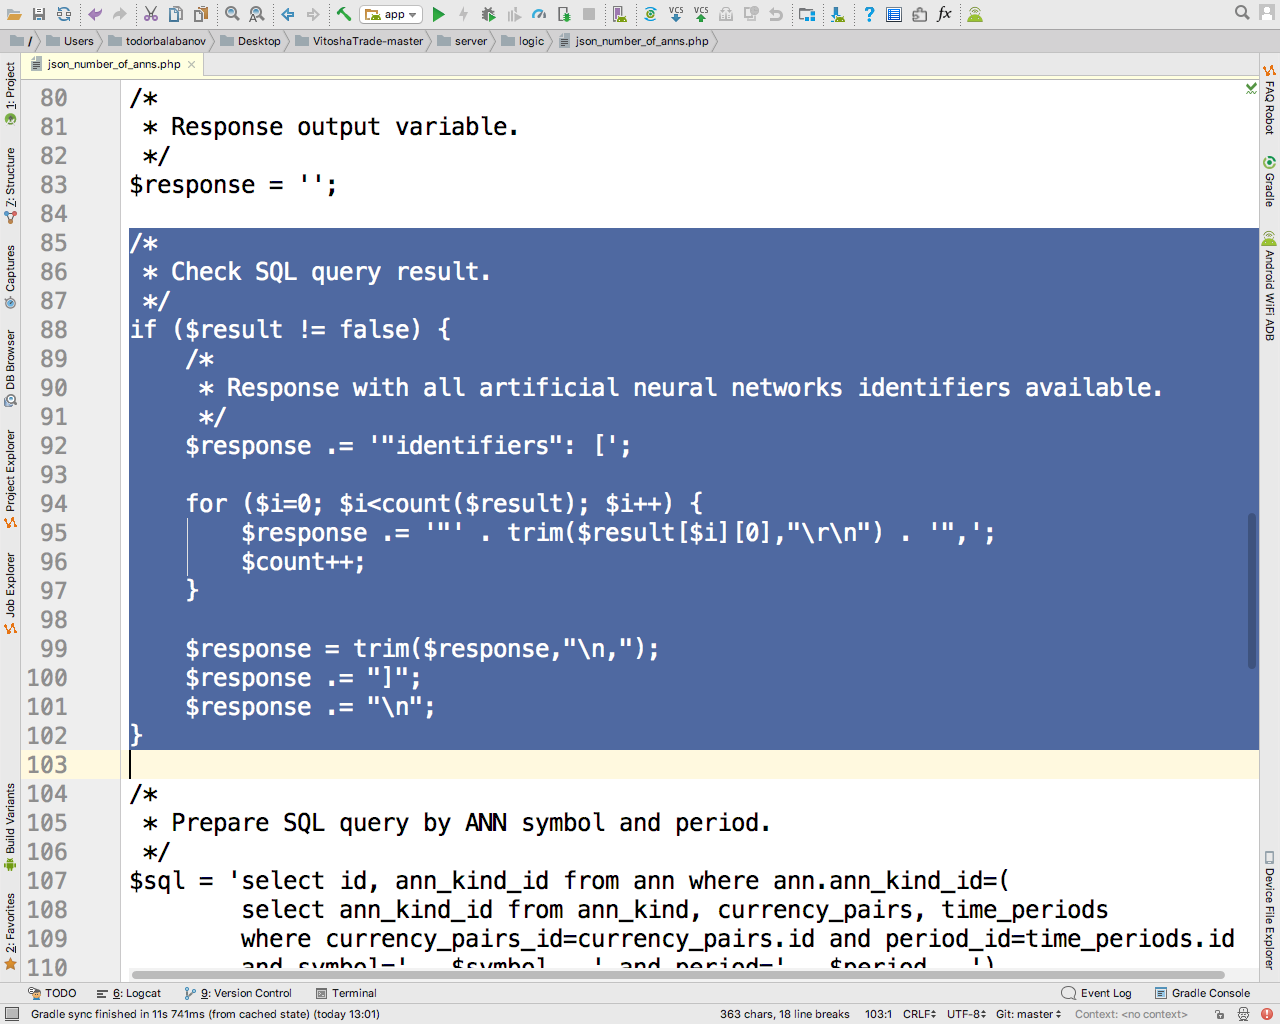
\includegraphics[height=0.45\pdfpageheight]{pic0135}
\caption{Pack the received values into a JSON message}
\label{fig:pic0135}
\end{figure}
\FloatBarrier

The resulting values are packed into a JSON message (Fig. \ref{fig:pic0135}).

\begin{figure}[h]
\centering
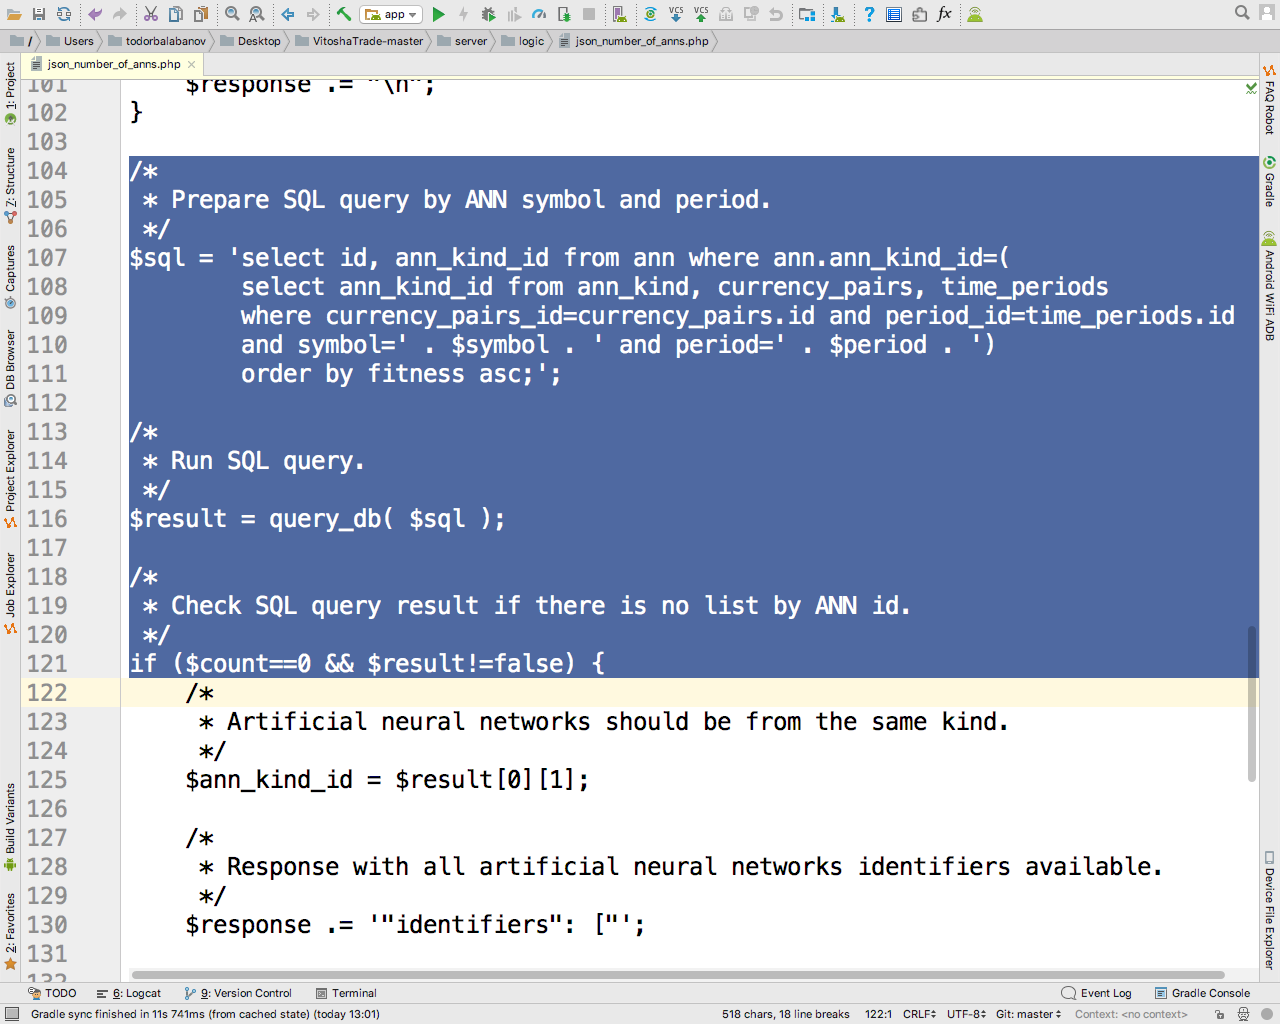
\includegraphics[height=0.45\pdfpageheight]{pic0136}
\caption{Check for instances by currency pair name and period}
\label{fig:pic0136}
\end{figure}
\FloatBarrier

Next is a check for instances by currency pair name and period. This list is only used if no subset is initially found (Fig. \ref{fig:pic0136}).

\begin{figure}[h]
\centering
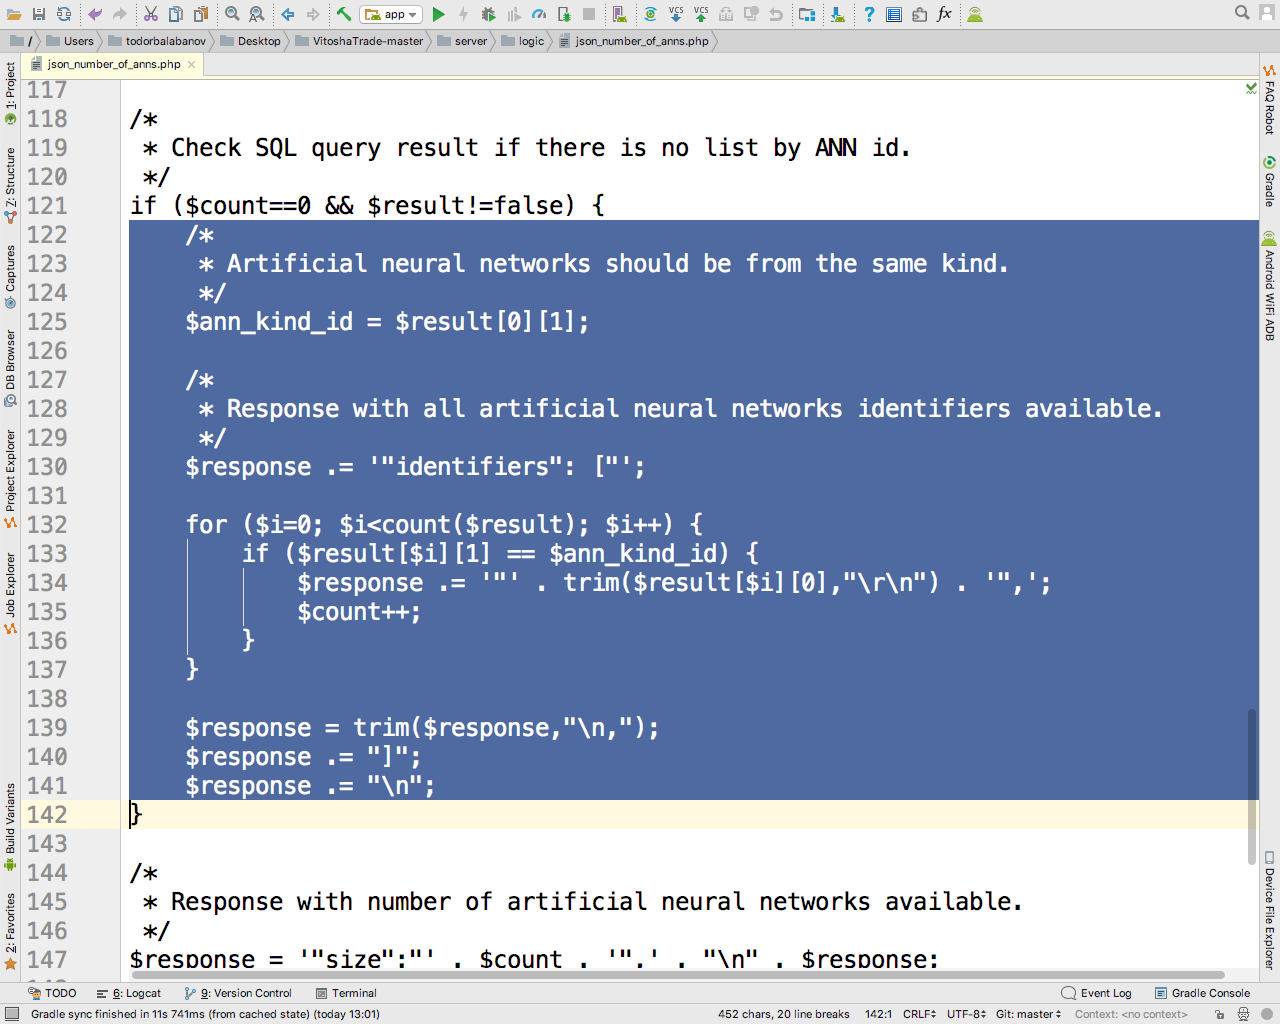
\includegraphics[height=0.45\pdfpageheight]{pic0137}
\caption{Pack the received values into a JSON message}
\label{fig:pic0137}
\end{figure}
\FloatBarrier

Packaging in a JSON message is analogous to the previous one (Fig. \ref{fig:pic0137}).

\begin{figure}[h]
\centering
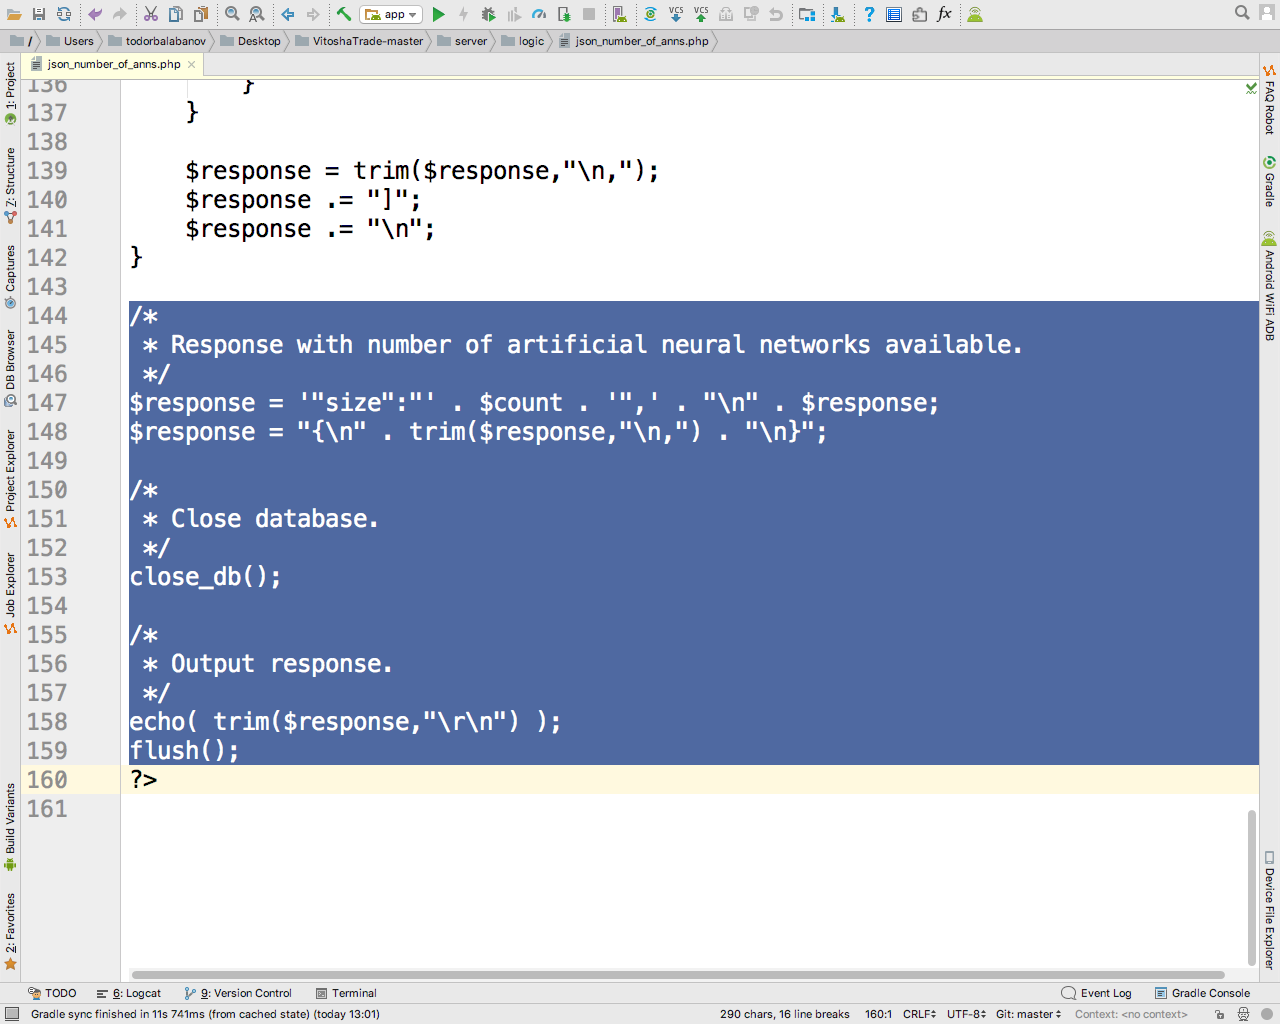
\includegraphics[height=0.45\pdfpageheight]{pic0138}
\caption{Send Result}
\label{fig:pic0138}
\end{figure}
\FloatBarrier

The script ends by closing the database connection, formatting, and sending the result to the client (Fig. \ref{fig:pic0138}).

\subsection{Loading number of training examples by currency pair information}

Determining the number of training examples is approached in a similar way by turning on the database module, checking the input arguments, and opening a connection to the database (Fig. \ref{fig:pic0139}).

\begin{figure}[h]
\centering
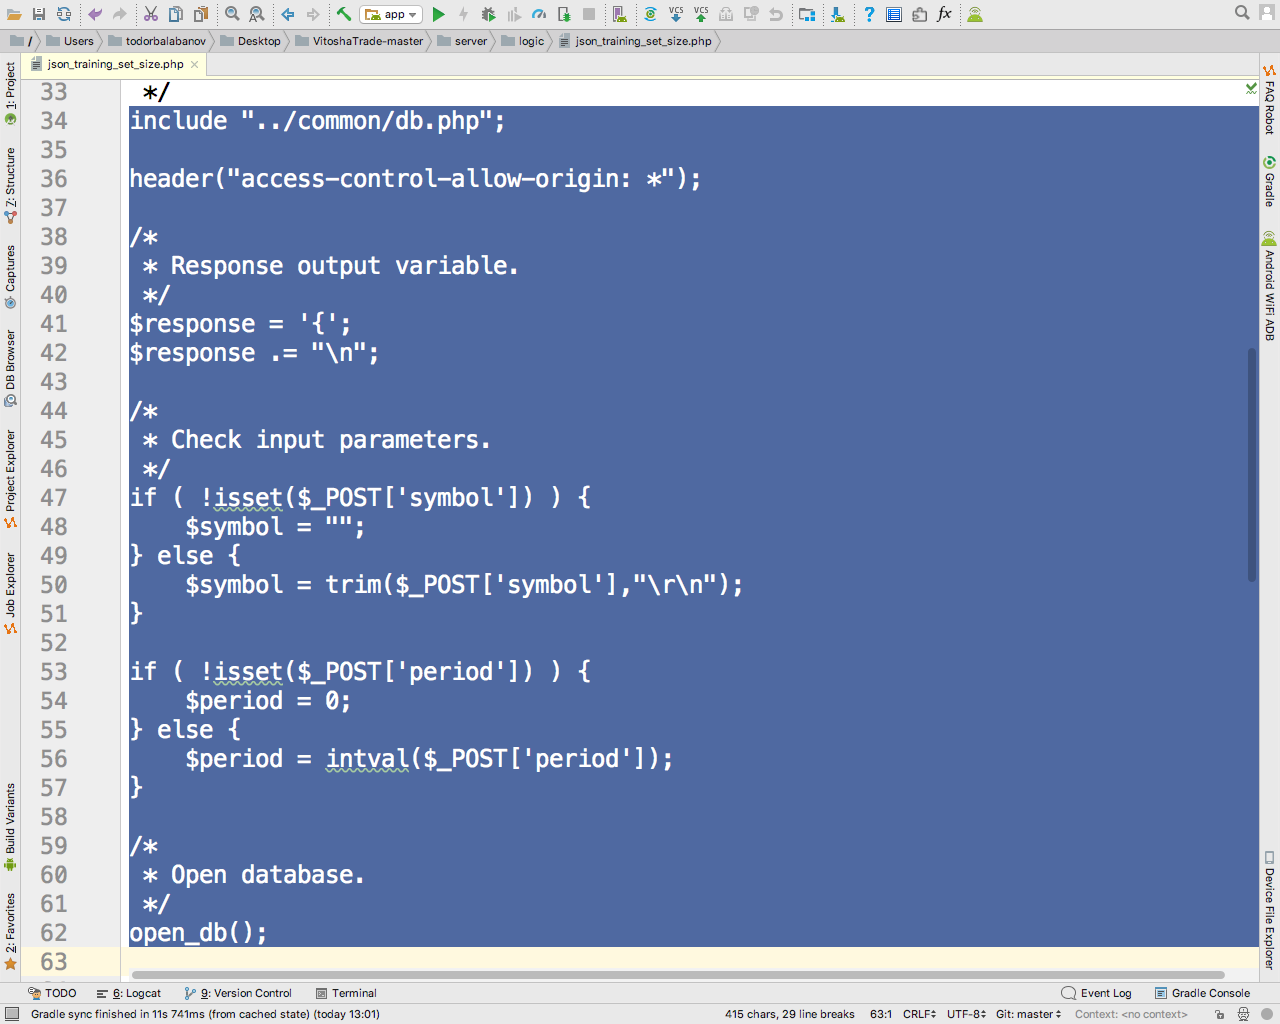
\includegraphics[height=0.45\pdfpageheight]{pic0139}
\caption{Number of currency information training examples}
\label{fig:pic0139}
\end{figure}
\FloatBarrier

Running the query may or may not find a suitable training set (Fig. \ref{fig:pic0140}).

\begin{figure}[h]
\centering
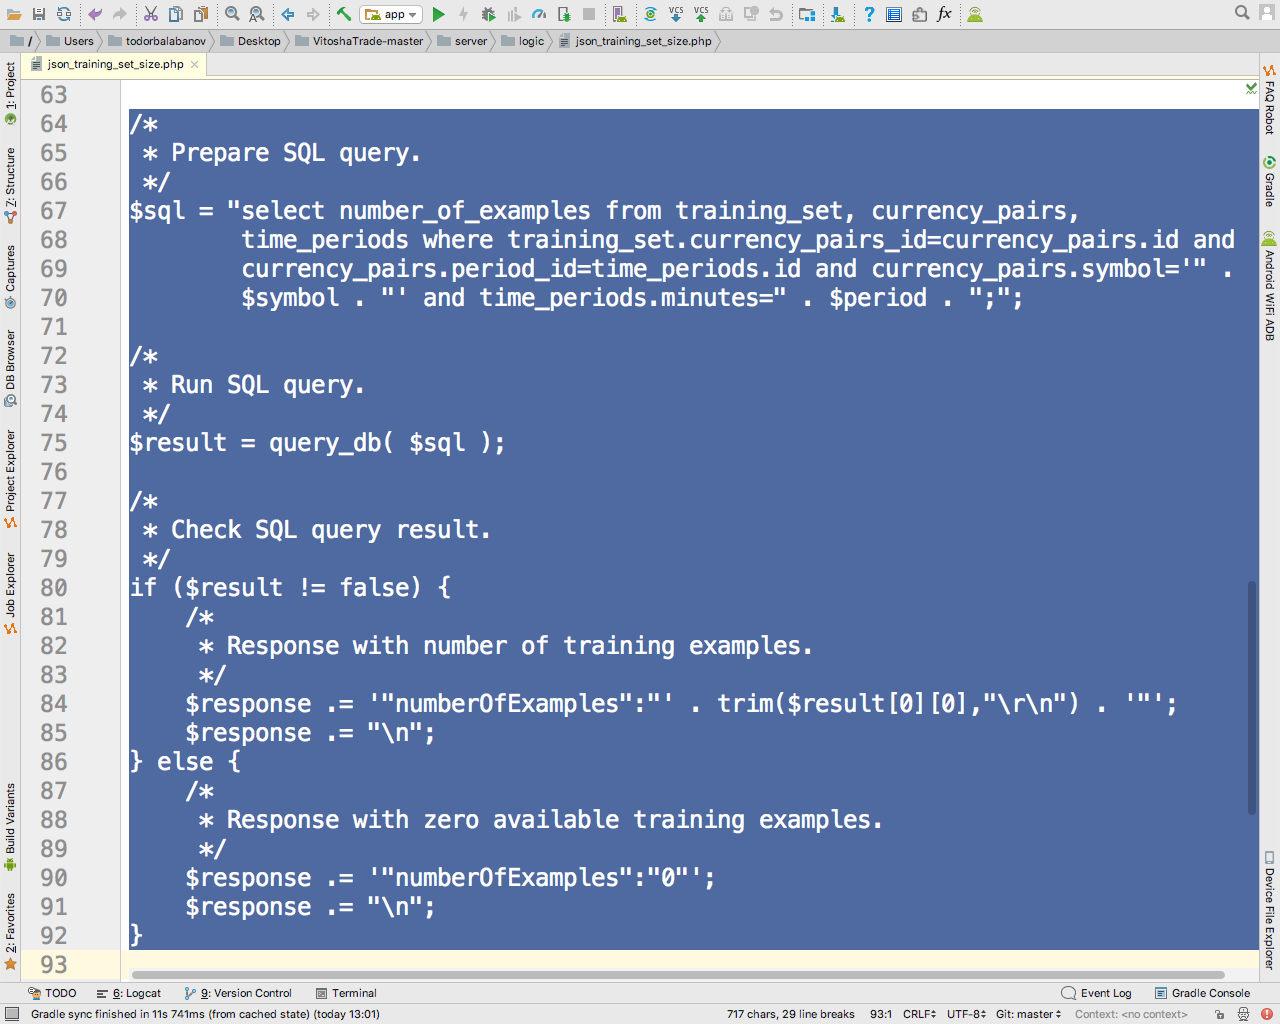
\includegraphics[height=0.45\pdfpageheight]{pic0140}
\caption{Request for number of training examples}
\label{fig:pic0140}
\end{figure}
\FloatBarrier

The script ends by closing the database connection, packaging and sending the response to the client (Fig. \ref{fig:pic0141}).

\begin{figure}[h]
\centering
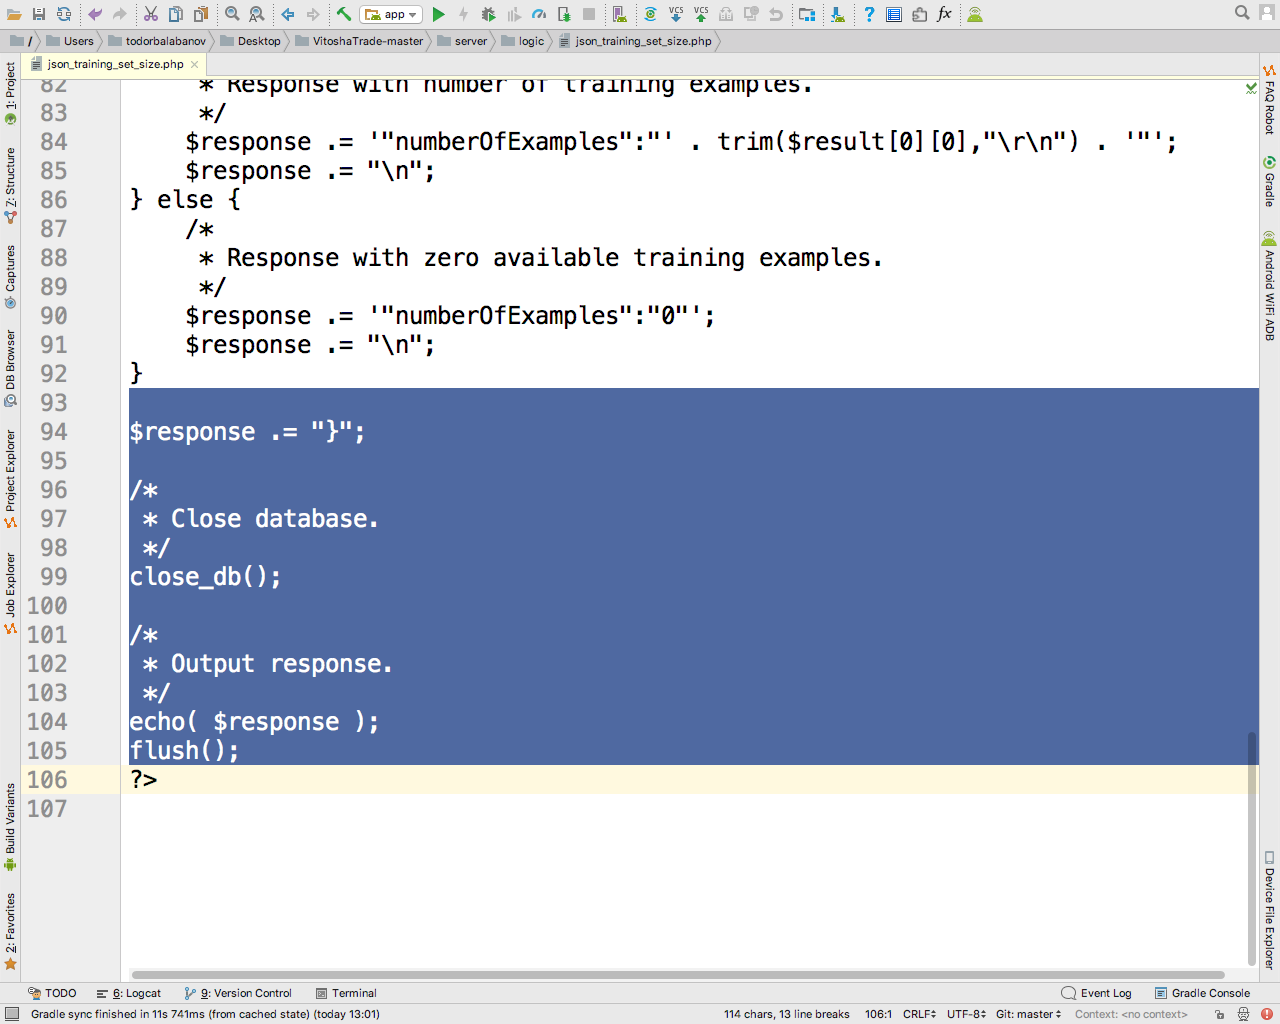
\includegraphics[height=0.45\pdfpageheight]{pic0141}
\caption{Send response to client}
\label{fig:pic0141}
\end{figure}
\FloatBarrier

\subsection{Storing an Artificial Neural Network Instance}

Storing an instance of the artificial neural network does not return a result for the execution of the operation, and therefore JSON is not used. After the database module is included, a more complex check of the input arguments is required, as they are more numerous and more complex (Fig. \ref{fig:pic0142}-\ref{fig:pic0146}) .

\begin{figure}[h]
\centering
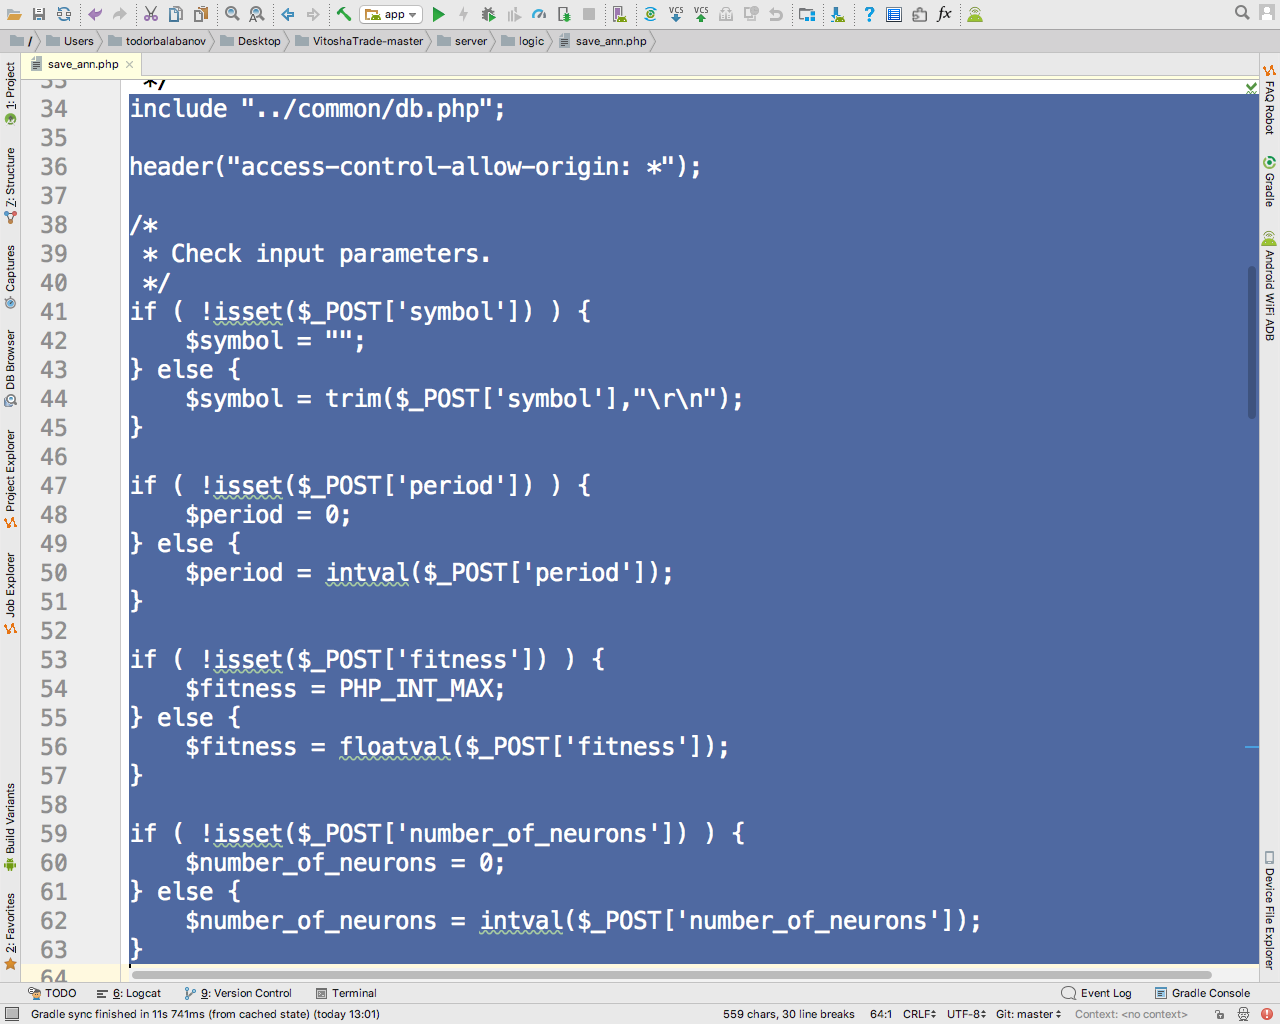
\includegraphics[height=0.45\pdfpageheight]{pic0142}
\caption{Validation of input arguments for currency pair, period, liveness and number of neurons}
\label{fig:pic0142}
\end{figure}
\FloatBarrier

\begin{figure}[h]
\centering
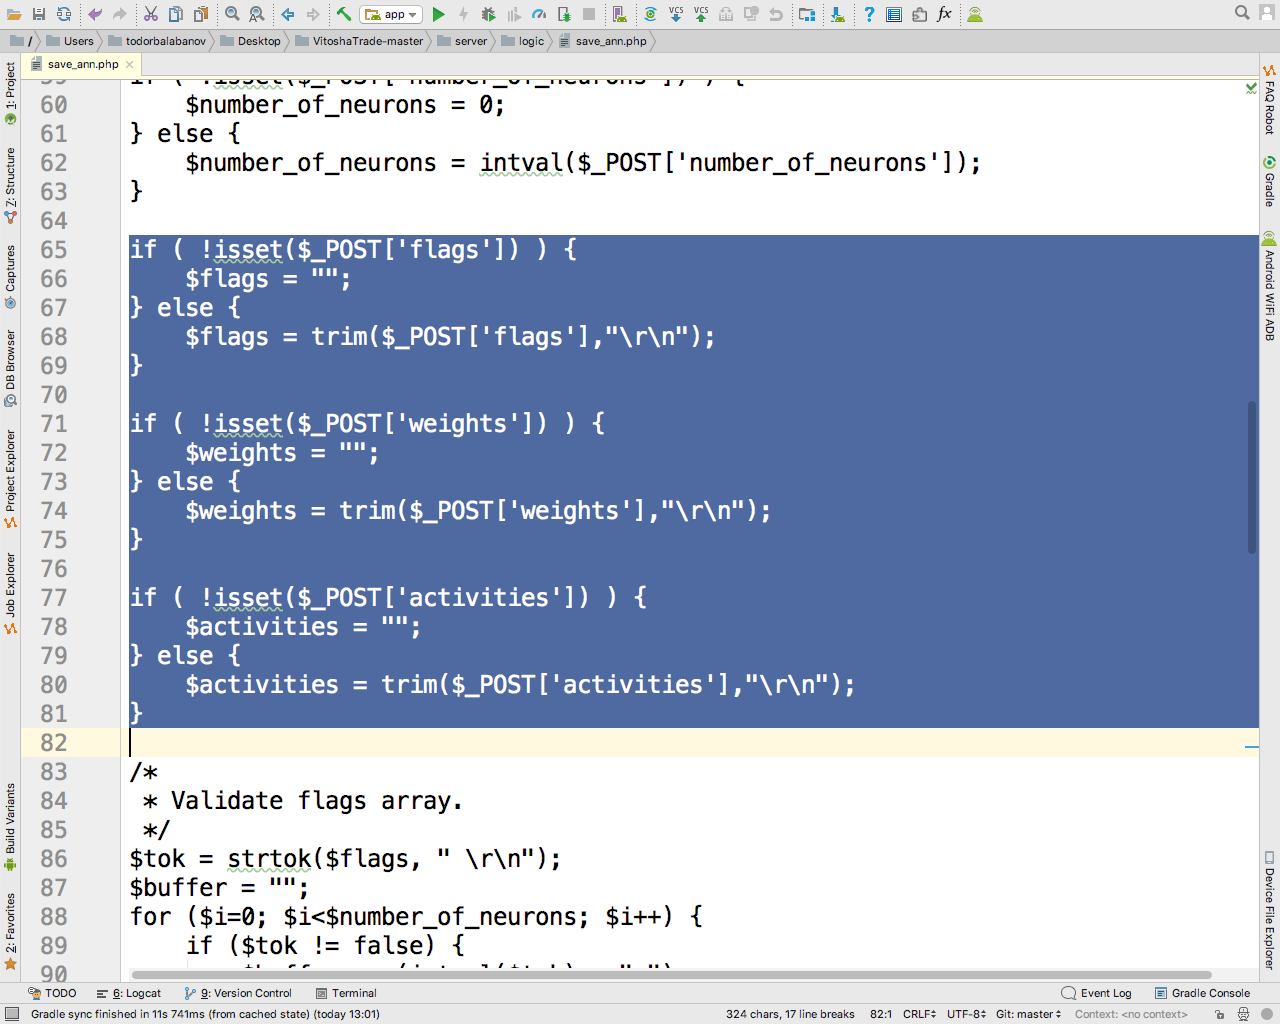
\includegraphics[height=0.45\pdfpageheight]{pic0143}
\caption{Checking input arguments for neuron flags, connections and weights between neurons}
\label{fig:pic0143}
\end{figure}
\FloatBarrier

\begin{figure}[h]
\centering
\includegraphics[height=0.45\pdfpageheight]{pic0144}
\caption{Checking for the type of each neuron}
\label{fig:pic0144}
\end{figure}
\FloatBarrier

\begin{figure}[h]
\centering
\includegraphics[height=0.45\pdfpageheight]{pic0145}
\caption{Checking for the value of each weight}
\label{fig:pic0145}
\end{figure}
\FloatBarrier

\begin{figure}[h]
\centering
\includegraphics[height=0.45\pdfpageheight]{pic0146}
\caption{Checking for the value of each link}
\label{fig:pic0146}
\end{figure}
\FloatBarrier

With this script, the checks are significantly more complicated, because in addition to the availability of the arguments, the numeric values that arrive from the client application are monitored.

\begin{figure}[h]
\centering
\includegraphics[height=0.45\pdfpageheight]{pic0147}
\caption{Storage of an artificial neural network instance}
\label{fig:pic0147}
\end{figure}
\FloatBarrier

The essence of the script is to open a connection to the database, execute a stored procedure, and close the connection to the database (Fig. \ref{fig:pic0147}).

\subsection{Saving an artificial neural network instance after retraining}

When a particular artificial neural network has undergone an additional training cycle and is sent to the remote server, it is reasonable to store the information only if it leads to an improvement in liveness.

\begin{figure}[h]
\centering
\includegraphics[height=0.45\pdfpageheight]{pic0158}
\caption{Validity check before storing the information}
\label{fig:pic0158}
\end{figure}
\FloatBarrier

The difference between the general artificial neural network storage procedure and the storage after additional training is in the verification of the best lifetime value achieved (Fig. \ref{fig:pic0158}).

\subsection{Storing training set}

Similarly, storing training examples does not return a JSON message, and the input validation code overrides the code for storing itself. Initially, the presence of the arguments is checked (Fig. \ref{fig:pic0148},\ref{fig:pic0149}).

\begin{figure}[h]
\centering
\includegraphics[height=0.45\pdfpageheight]{pic0148}
\caption{Checking arguments for currency pair, period, number of examples and timestamps}
\label{fig:pic0148}
\end{figure}
\FloatBarrier

\begin{figure}[h]
\centering
\includegraphics[height=0.45\pdfpageheight]{pic0149}
\caption{Checking arguments for open, low, high, close and traded volume}
\label{fig:pic0149}
\end{figure}
\FloatBarrier

Each of the arrays passes an additional check for the values it contains (Fig. \ref{fig:pic0150}-\ref{fig:pic0152}).

\begin{figure}[h]
\centering
\includegraphics[height=0.45\pdfpageheight]{pic0150}
\caption{Checking values for timestamps and open levels}
\label{fig:pic0150}
\end{figure}
\FloatBarrier

\begin{figure}[h]
\centering
\includegraphics[height=0.45\pdfpageheight]{pic0151}
\caption{Checking the values for the lowest and highest level reached}
\label{fig:pic0151}
\end{figure}
\FloatBarrier

\begin{figure}[h]
\centering
\includegraphics[height=0.45\pdfpageheight]{pic0152}
\caption{Checking closing values and traded volume}
\label{fig:pic0152}
\end{figure}
\FloatBarrier

The script itself opens a connection to the database, executes a stored procedure, and closes the connection to the database (Fig. \ref{fig:pic0153}).

\begin{figure}[h]
\centering
\includegraphics[height=0.45\pdfpageheight]{pic0153}
\caption{Store training set}
\label{fig:pic0153}
\end{figure}
\FloatBarrier
